% images.tex - All figure definitions for the MASK documentation

% Introduction figures
\begin{figure}[!htbp]
    \centering
    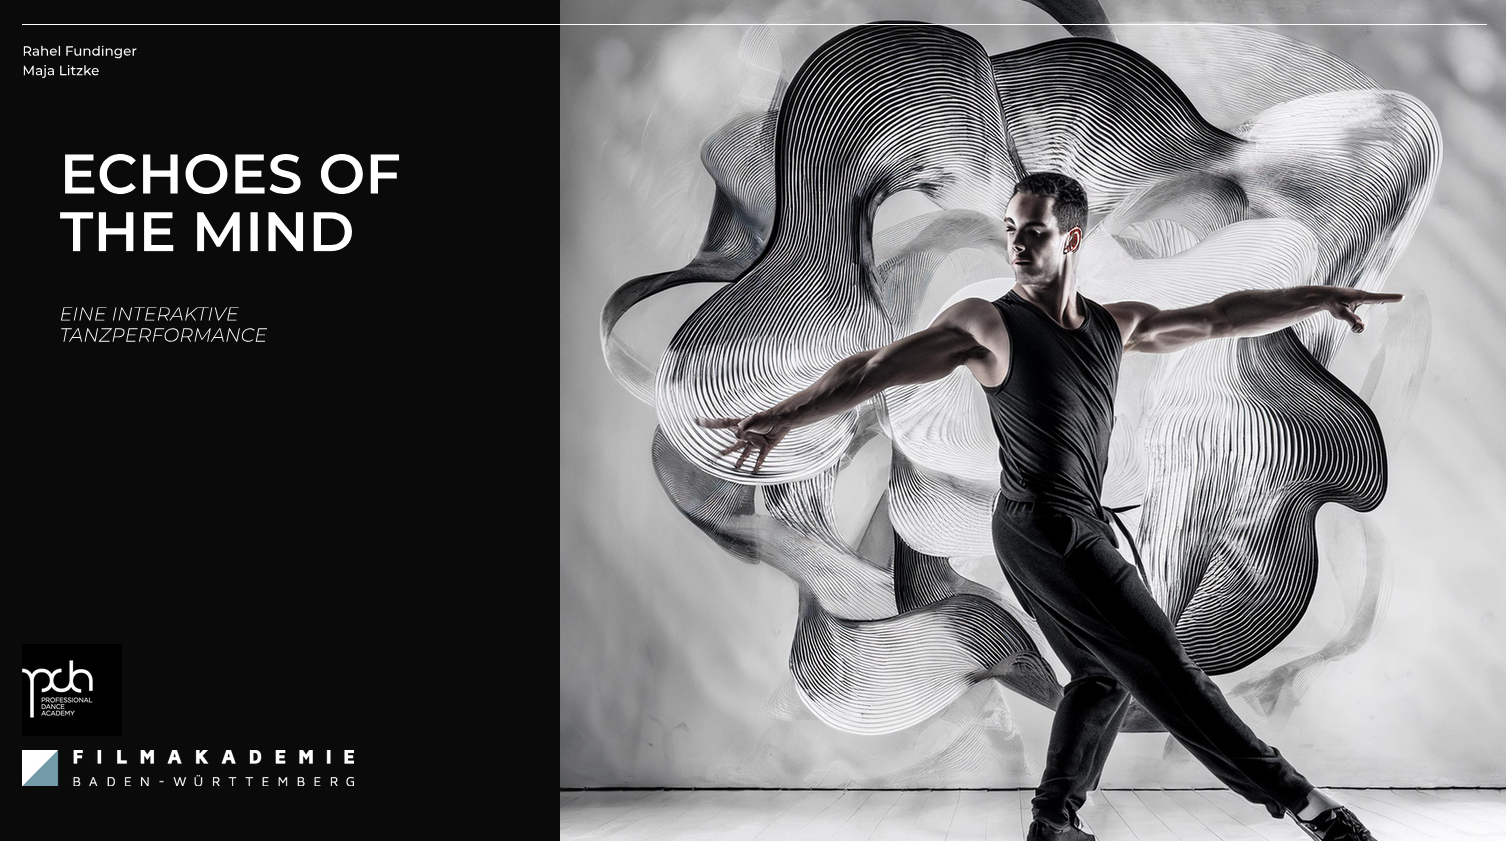
\includegraphics[width=0.6\textwidth,height=0.25\textheight,keepaspectratio]{images/EchoesOfTheMind_startbild.png}
    \caption{MoodBoard-Startbild des Projektes \glqq Echoes of the Mind\grqq{}}
    \label{fig:echoes_startbild}
\end{figure}

\begin{figure}[!htbp]
    \centering
    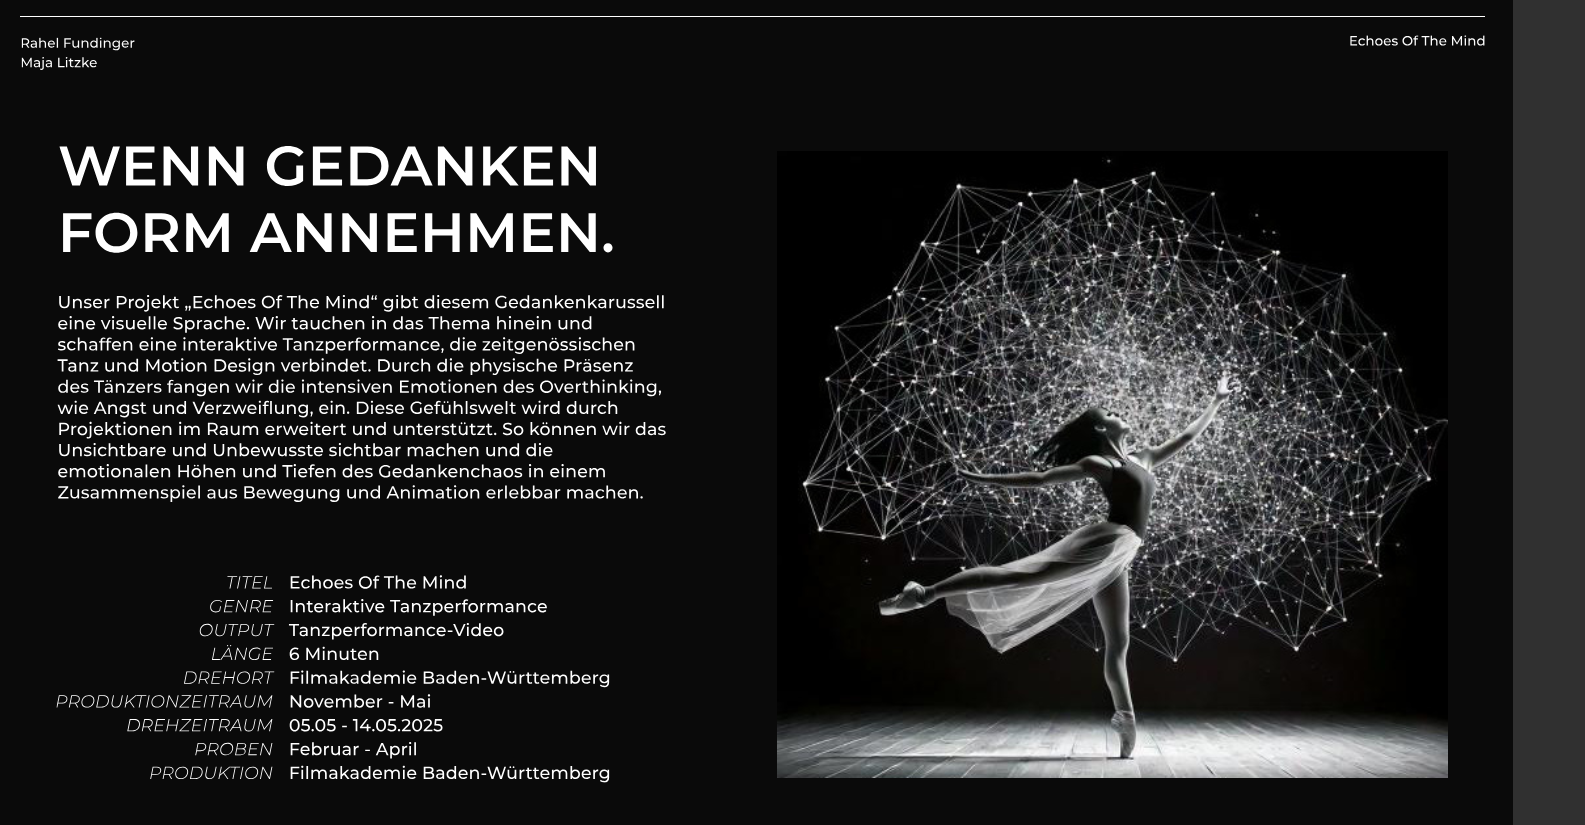
\includegraphics[width=0.6\textwidth,height=0.25\textheight,keepaspectratio]{images/EchoesOfTheMind_mood.png}
    \caption{K�nstlerische Vision: Emotionale Visualisierungskonzepte f�r \glqq Echoes of the Mind\grqq{}}
    \label{fig:echoes_mood}
\end{figure}

% Sprint 1 figures
\begin{figure}[!htbp]
    \centering
    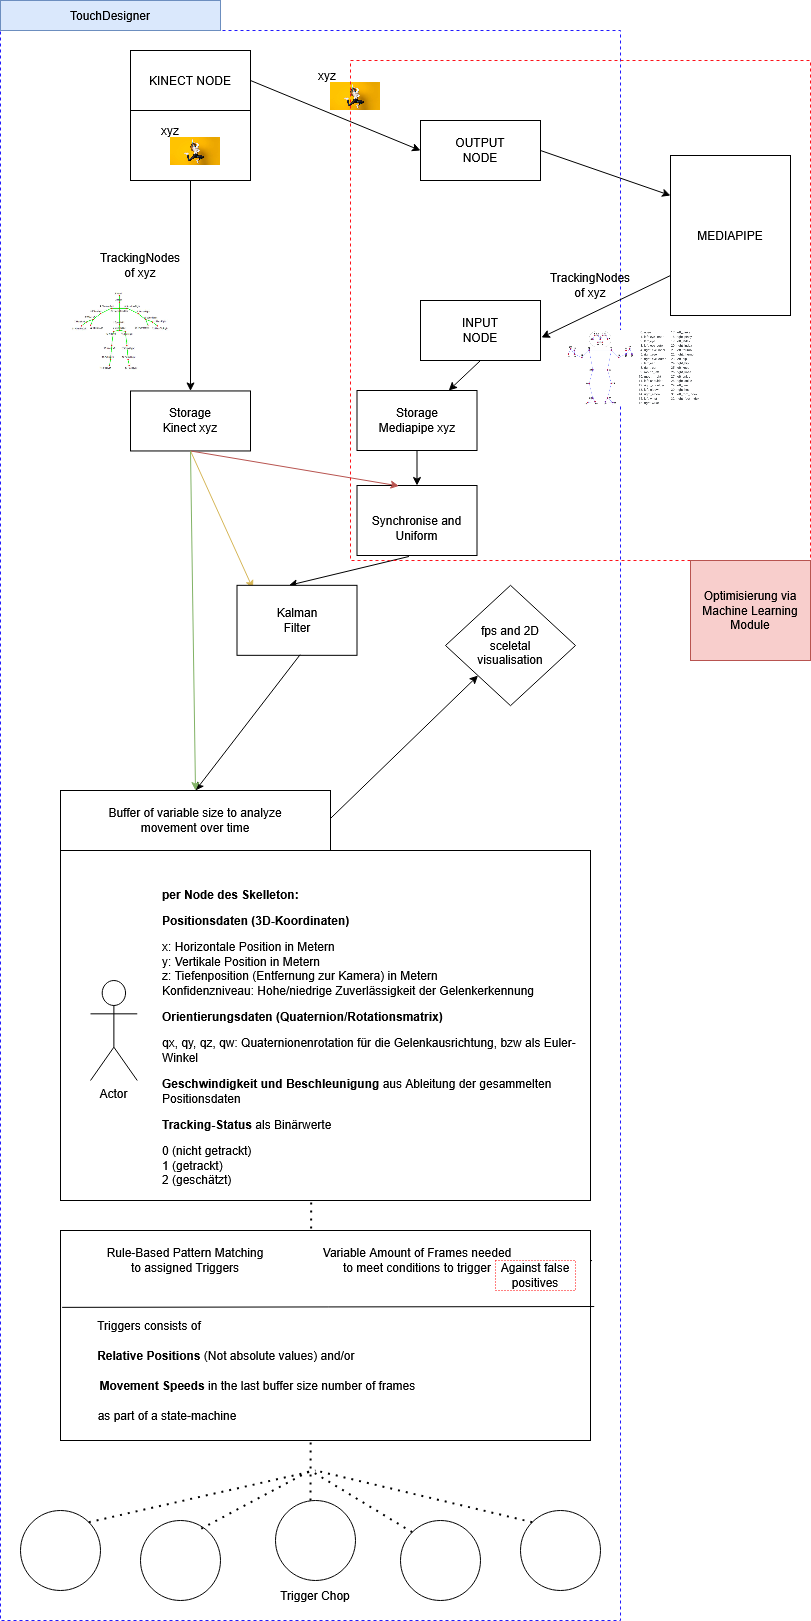
\includegraphics[width=0.6\textwidth,height=0.25\textheight,keepaspectratio]{images/MASK.png}
    \caption{M.A.S.K. Systemarchitektur: Analyse- und Triggerprozess}
    \label{fig:mask_architecture}
\end{figure}

% Sprint 2 figures
\begin{figure}[!htbp]
    \centering
    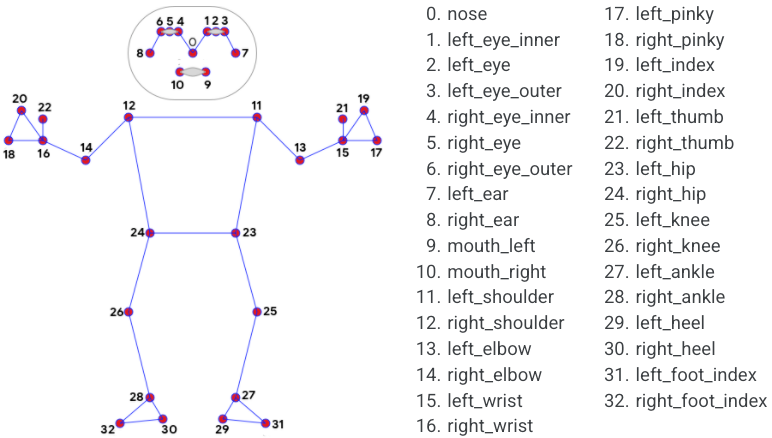
\includegraphics[width=0.6\textwidth,height=0.25\textheight,keepaspectratio]{images/mediapipeNODES.png}
    \caption{MediaPipe Skeleton-Node-Ausgabe mit Koordinaten und Confidence-Werten}
    \label{fig:mediapipe_nodes}
\end{figure}

\begin{figure}[!htbp]
    \centering
    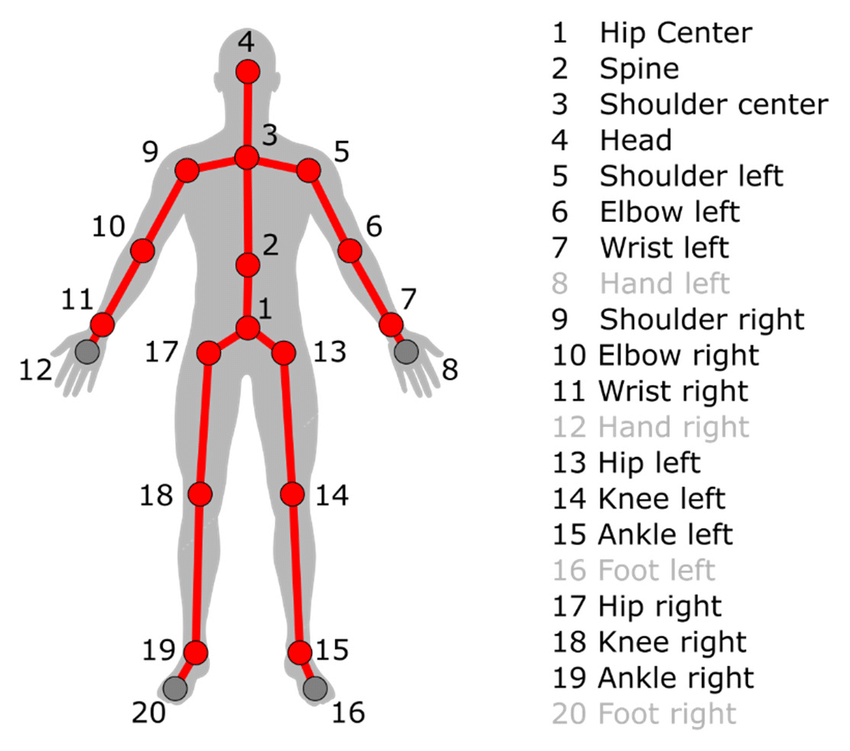
\includegraphics[width=0.6\textwidth,height=0.25\textheight,keepaspectratio]{images/kinect_nodes.png}
    \caption{Kinect V2 Skeleton-Visualisierung mit Node-Nummerierung}
    \label{fig:kinect_nodes}
\end{figure}

\begin{figure}[!htbp]
    \centering
    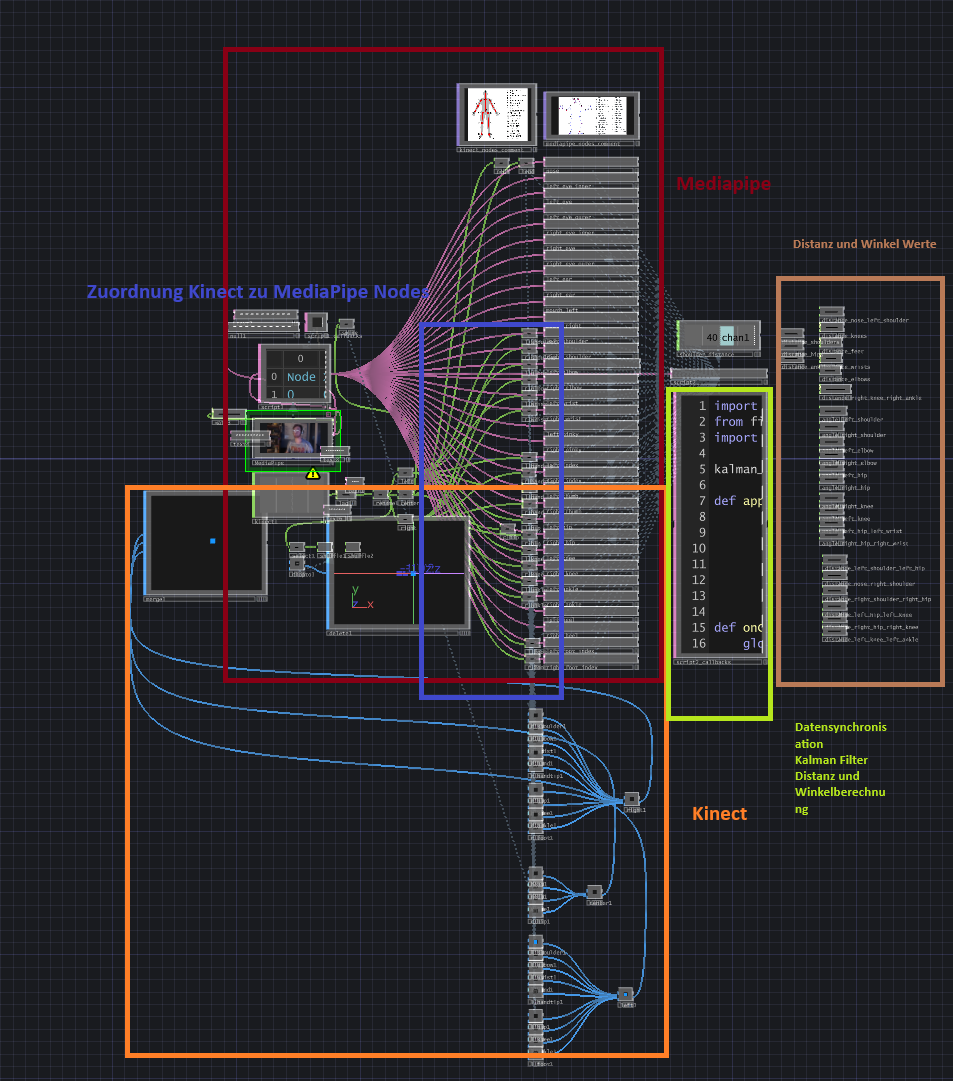
\includegraphics[width=0.6\textwidth,height=0.25\textheight,keepaspectratio]{images/docupictures/KinectMediaPipe_Testing.png}
    \caption{TouchDesigner-Interface f�r komparative Tracking-Tests}
    \label{fig:testing_interface}
\end{figure}

% Sprint 3 figures
\begin{figure}[!htbp]
    \centering
    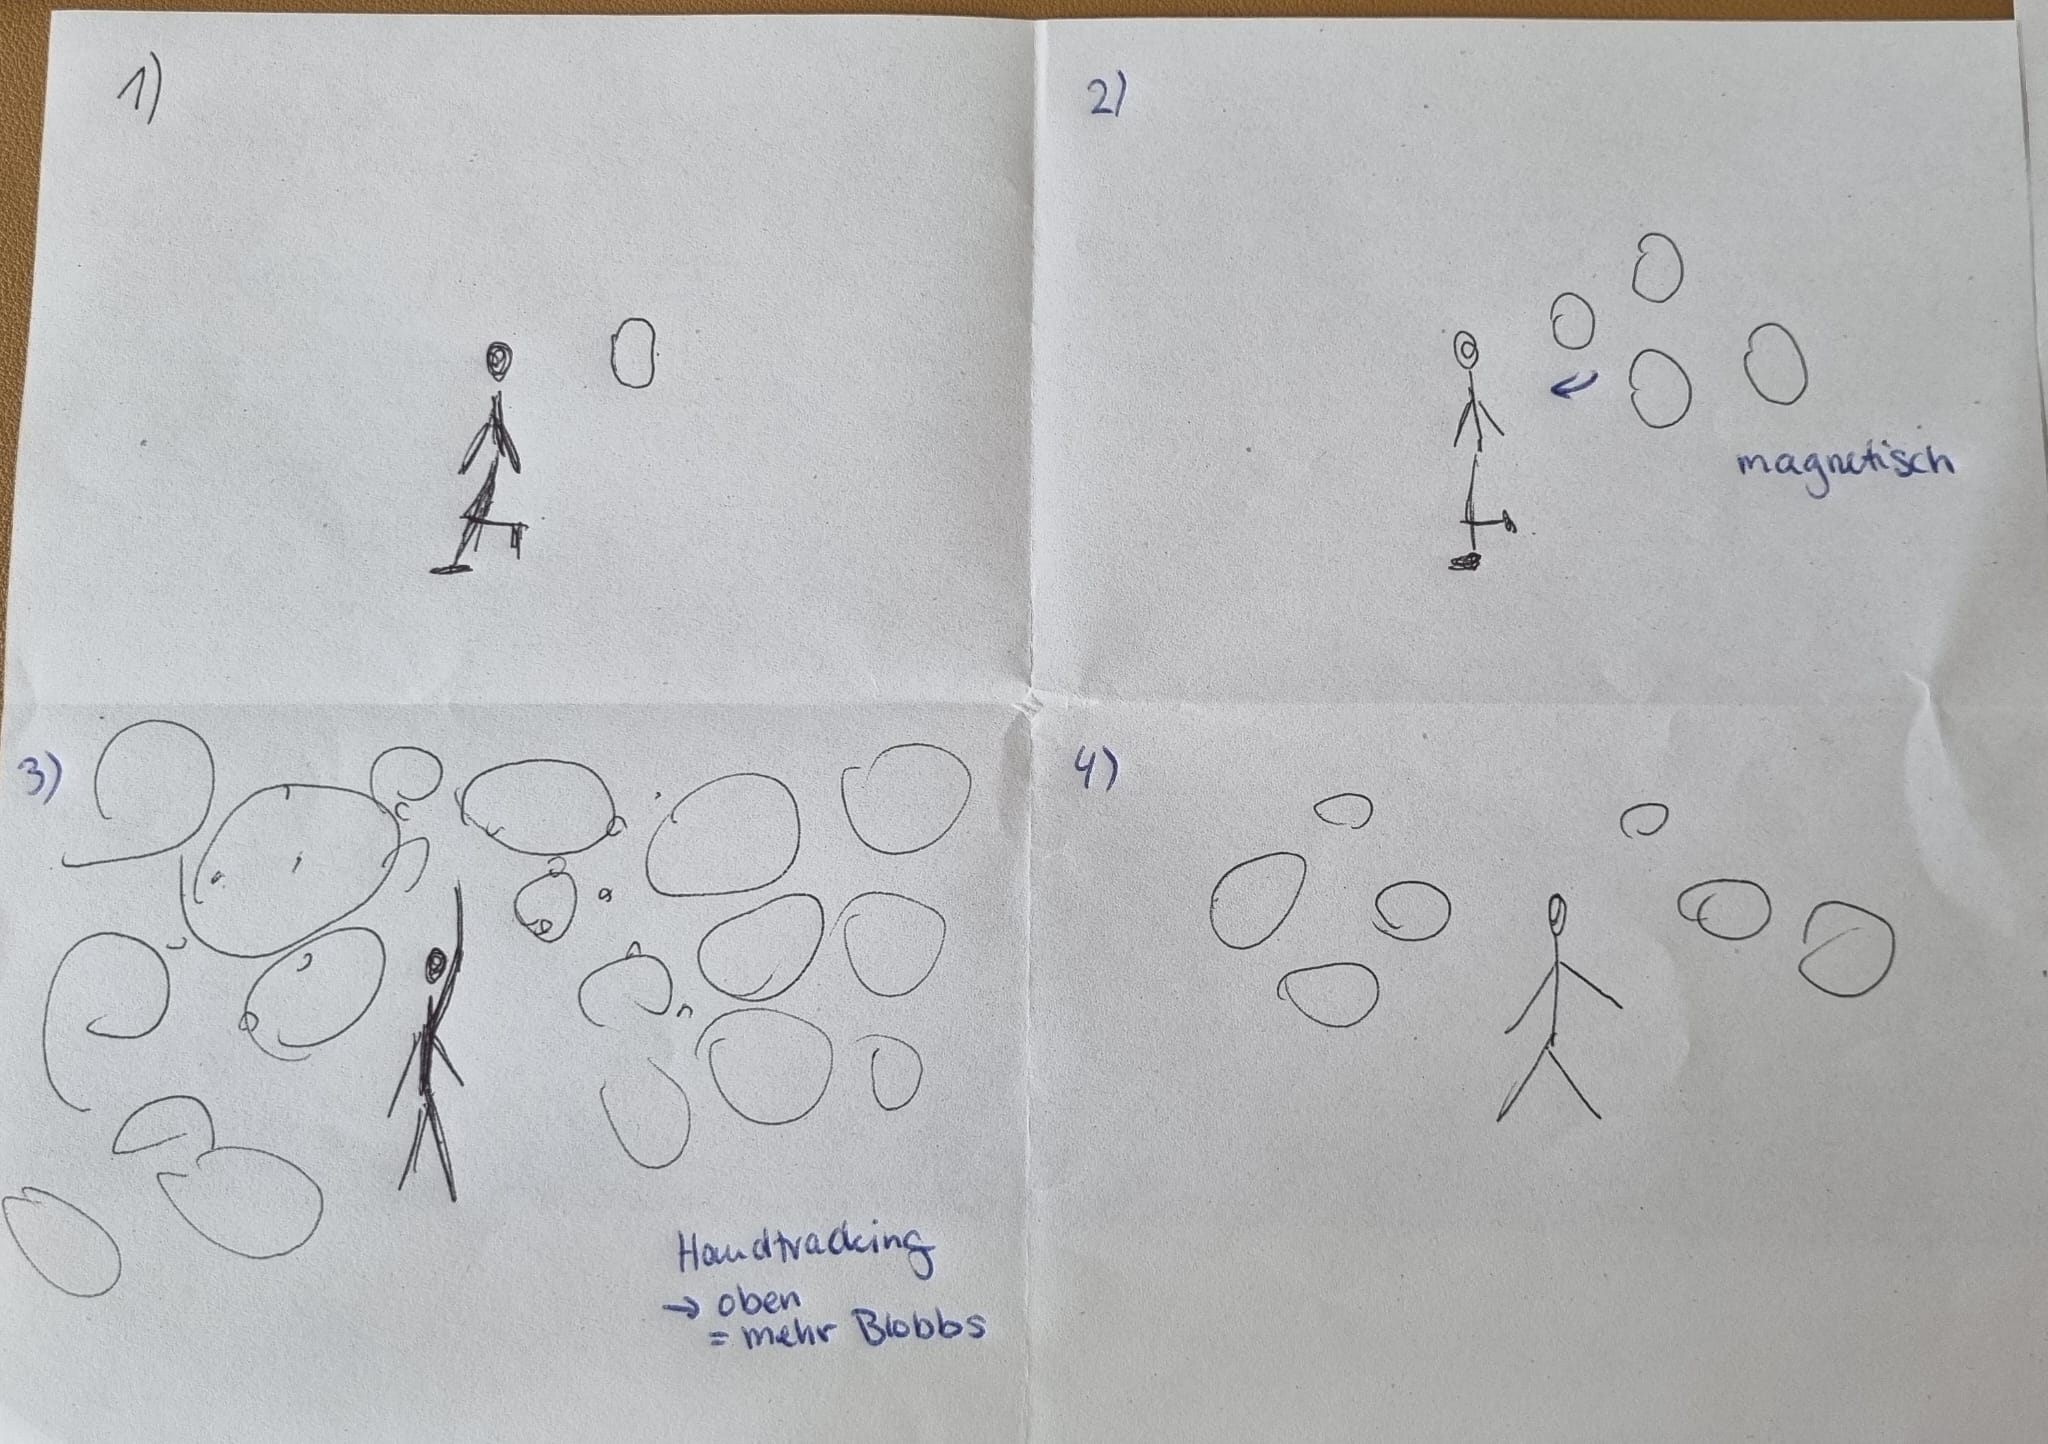
\includegraphics[width=0.6\textwidth,height=0.25\textheight,keepaspectratio]{images/Sprint3_1.jpg}
    \caption{Skalierungskonzept: Gr��enresponsive Visual-Transformation}
    \label{fig:scaling_concept}
\end{figure}

\begin{figure}[!htbp]
    \centering
    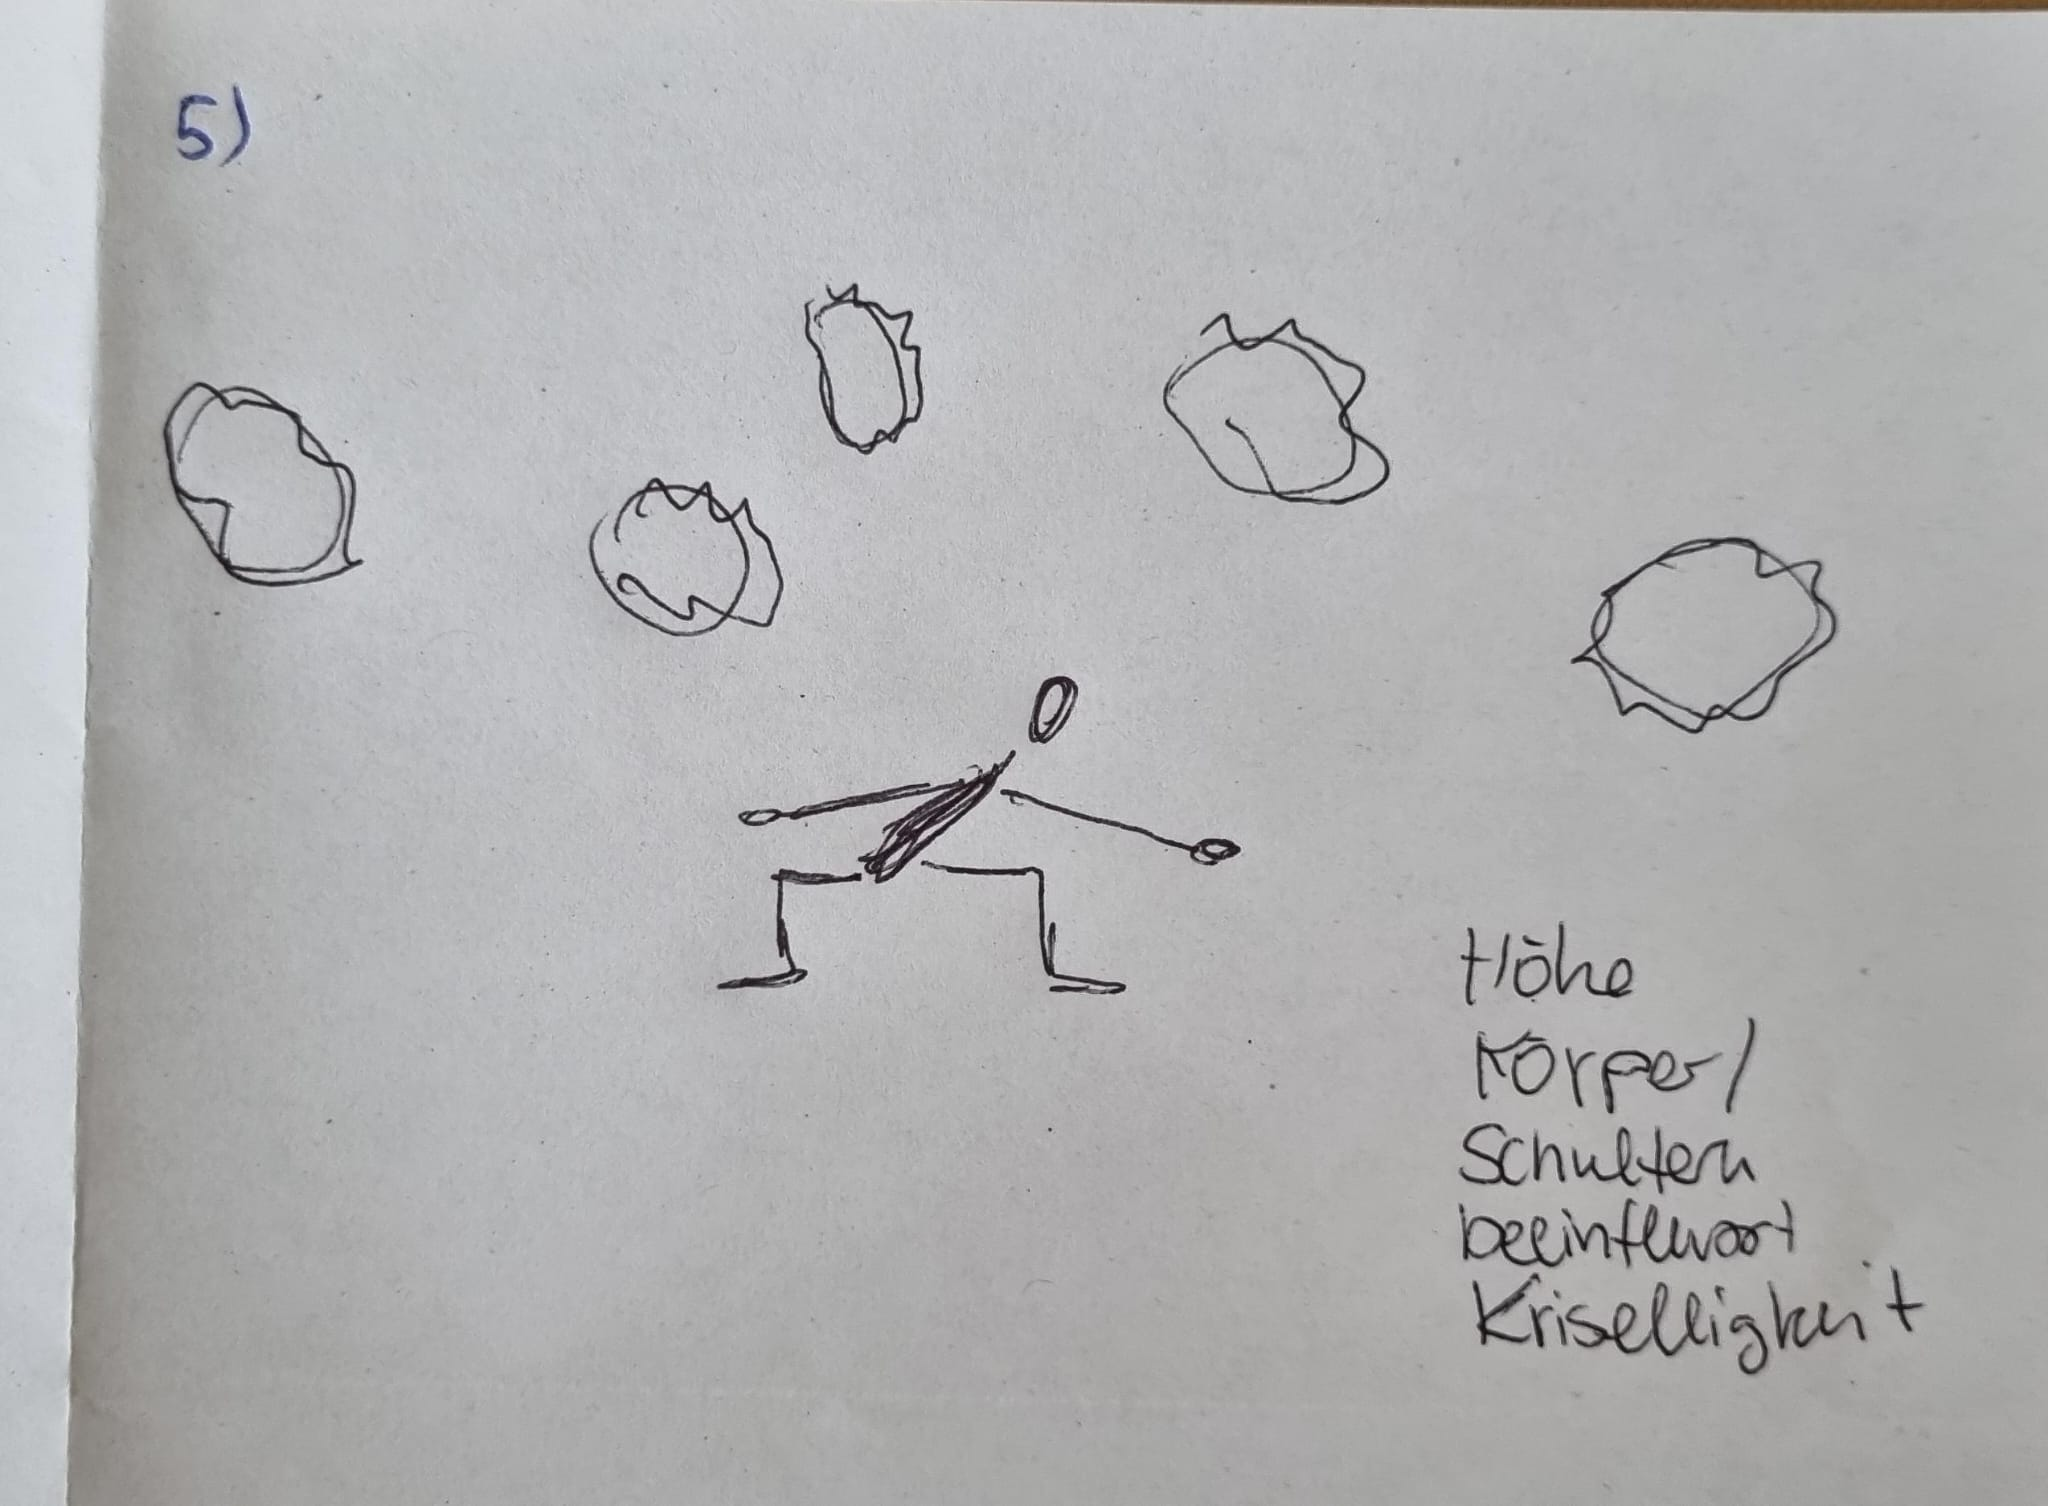
\includegraphics[width=0.6\textwidth,height=0.25\textheight,keepaspectratio]{images/Sprint3_2.jpg}
    \caption{R�umliche Verteilung: Externe Visual-Positionierung um Performer}
    \label{fig:external_positioning}
\end{figure}

\begin{figure}[!htbp]
    \centering
    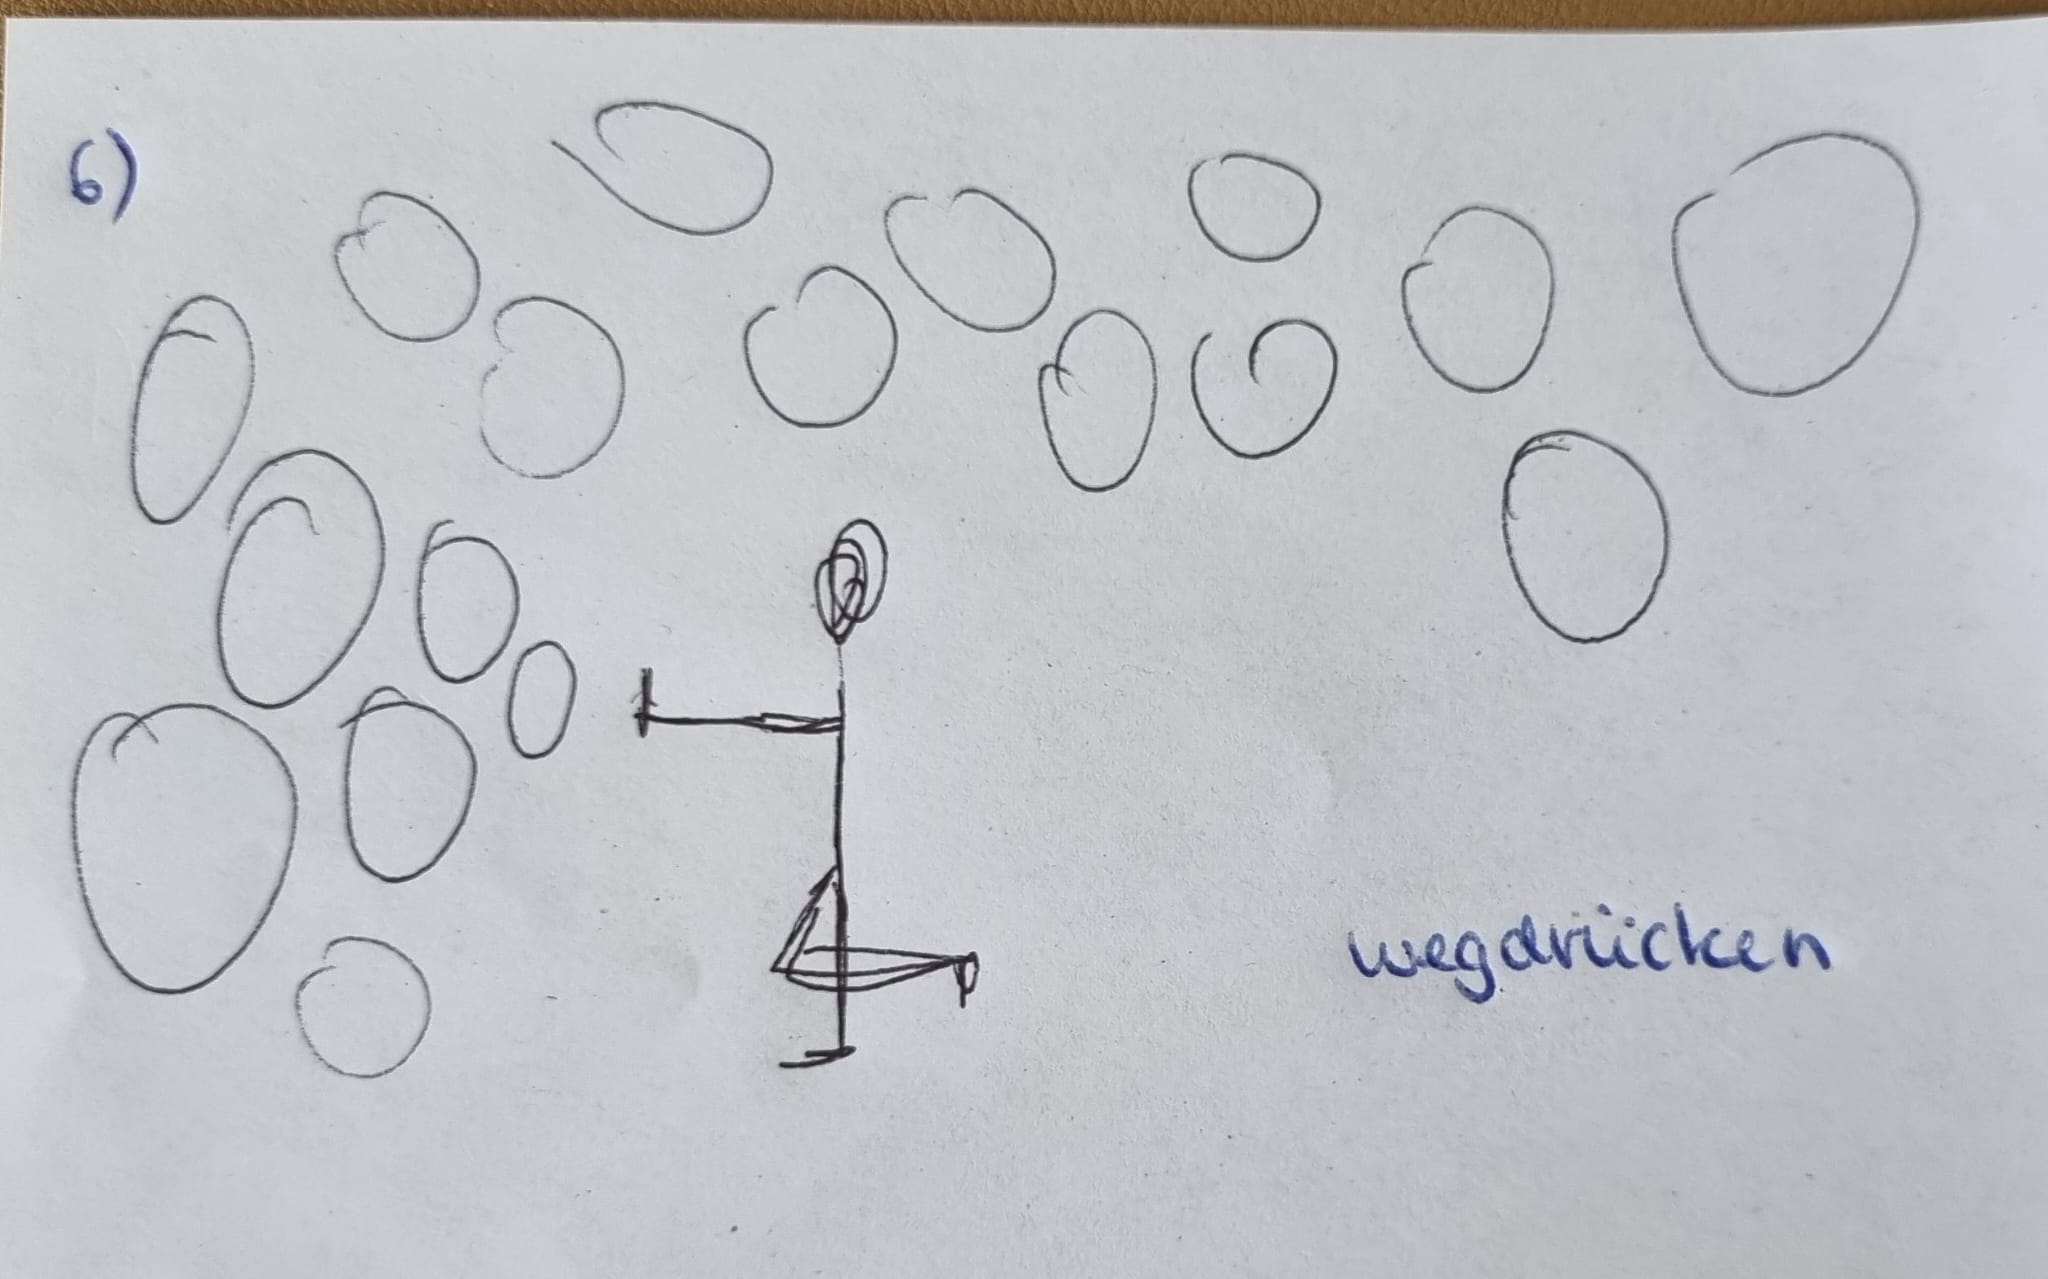
\includegraphics[width=0.6\textwidth,height=0.25\textheight,keepaspectratio]{images/Sprint3_3.jpg}
    \caption{Magnetische Interaktion: Dynamische Visual-Performer-Relation}
    \label{fig:magnetic_interaction}
\end{figure}

\begin{figure}[!htbp]
    \centering
    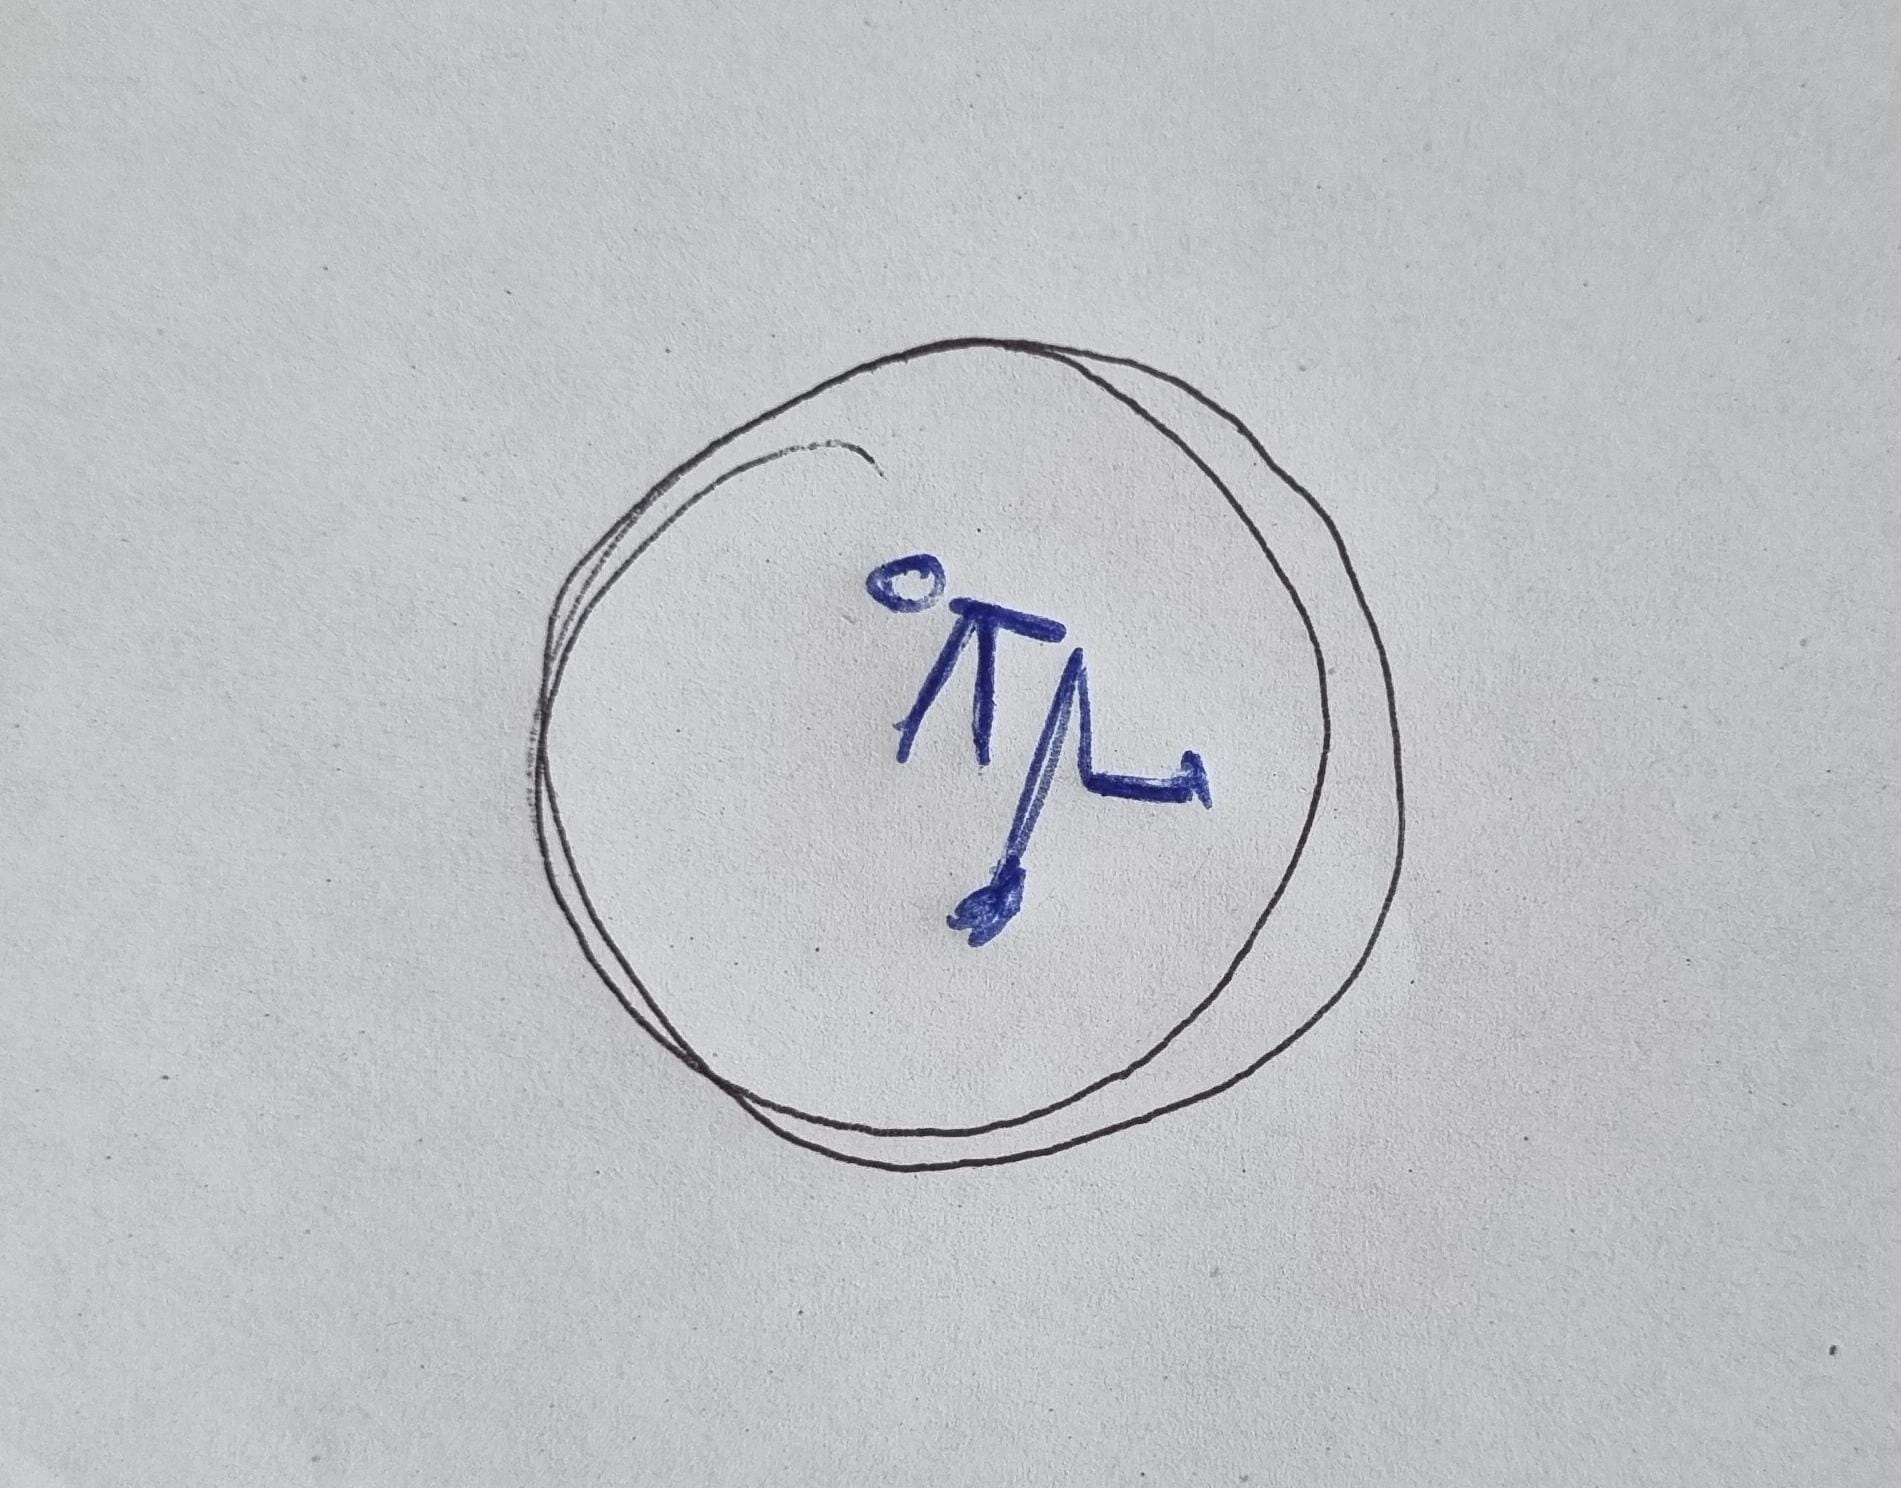
\includegraphics[width=0.6\textwidth,height=0.25\textheight,keepaspectratio]{images/Sprint3_4.jpg}
    \caption{Bewegungsresponsive Systeme: Performative Visual-Modulation}
    \label{fig:movement_responsive}
\end{figure}

\begin{figure}[!htbp]
    \centering
    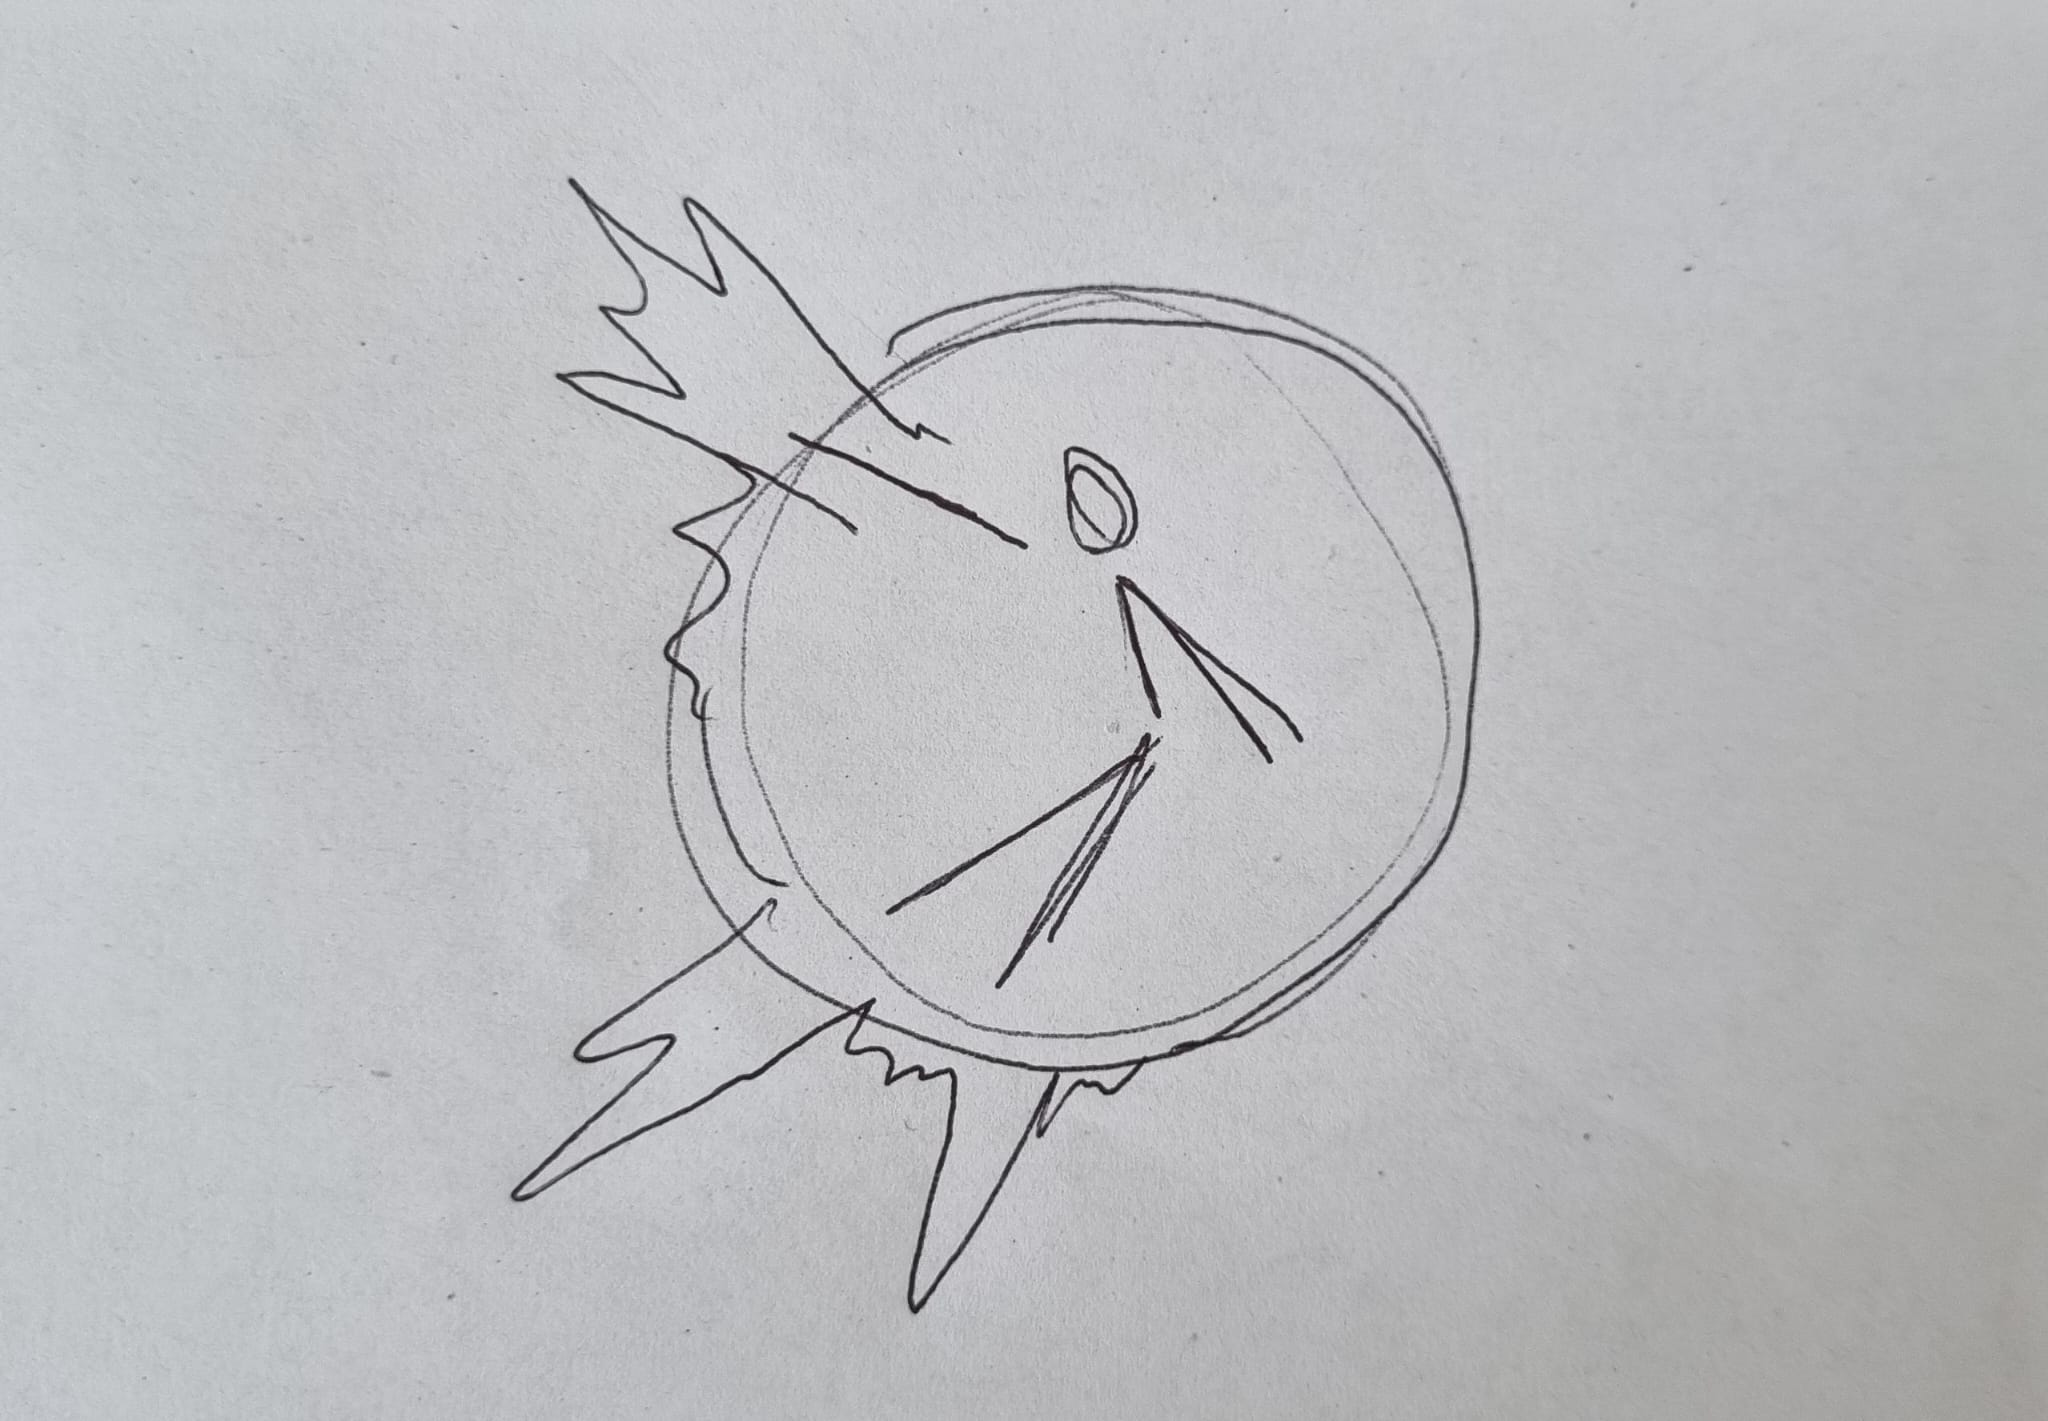
\includegraphics[width=0.6\textwidth,height=0.25\textheight,keepaspectratio]{images/Sprint3_5.jpg}
    \caption{Komposit-Effekte: Multi-Layer-Visual-Orchestrierung}
    \label{fig:composite_effects}
\end{figure}

% Sprint 4 figures
\begin{figure}[!htbp]
    \centering
    % \includegraphics[width=0.6\textwidth,height=0.25\textheight,keepaspectratio]{images/debug_visualization.png}
    \caption{Debug-Visualisierung: MediaPipe Skeleton-Nodes mit Confidence-Overlays}
    \label{fig:debug_viz}
\end{figure}

% Sprint 5 figures
\begin{figure}[!htbp]
    \centering
    \includegraphics[width=0.6\textwidth,height=0.25\textheight,keepaspectratio]{images/docupictures/Finished_MediaPipeContainer_mitErkl�rungen.png}
    \caption{M.A.S.K. Haupt-Interface: MediaPipe Integration mit Debug-Visualisierung}
    \label{fig:main_interface}
\end{figure}

\begin{figure}[!htbp]
    \centering
    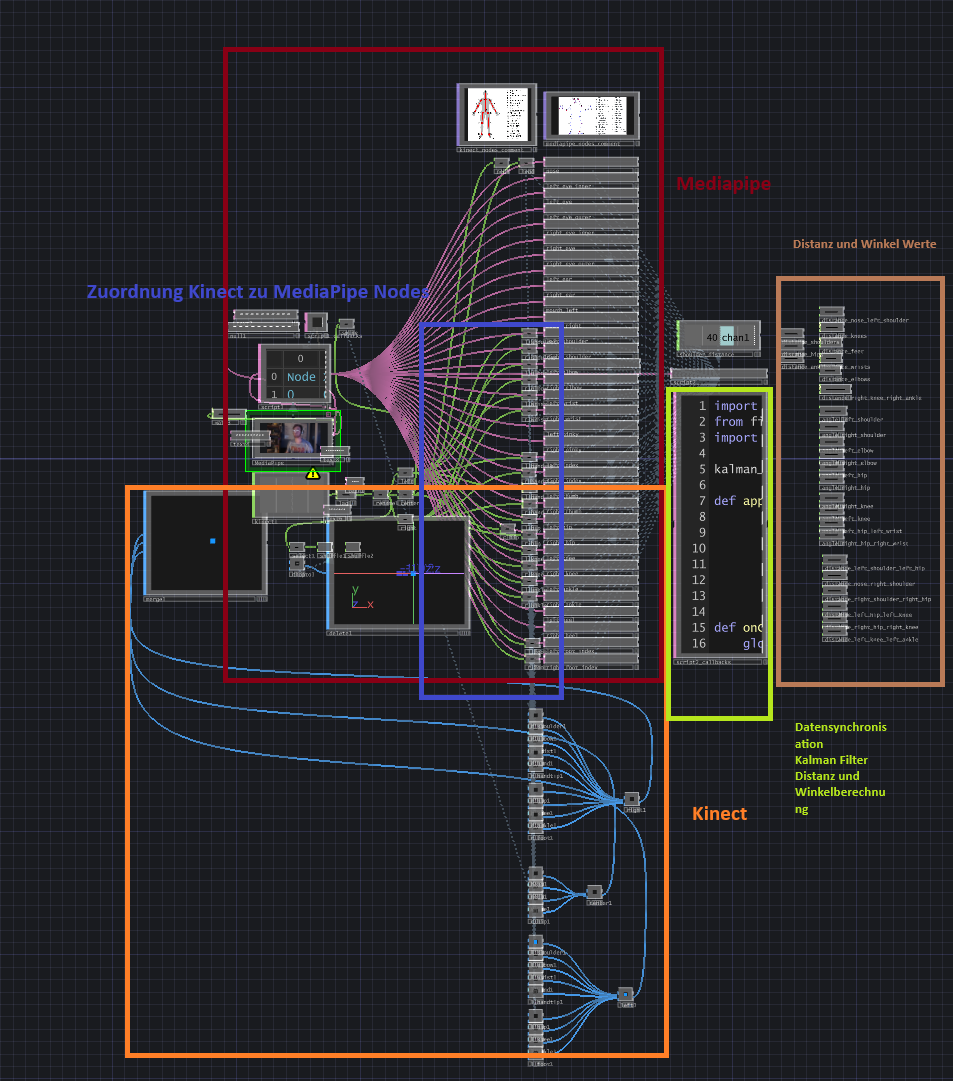
\includegraphics[width=0.6\textwidth,height=0.25\textheight,keepaspectratio]{images/docupictures/KinectMediaPipe_Testing.png}
    \caption{Komparative Tracking-Tests: MediaPipe vs. Kinect Evaluation}
    \label{fig:tracking_comparison}
\end{figure}

\begin{figure}[!htbp]
    \centering
    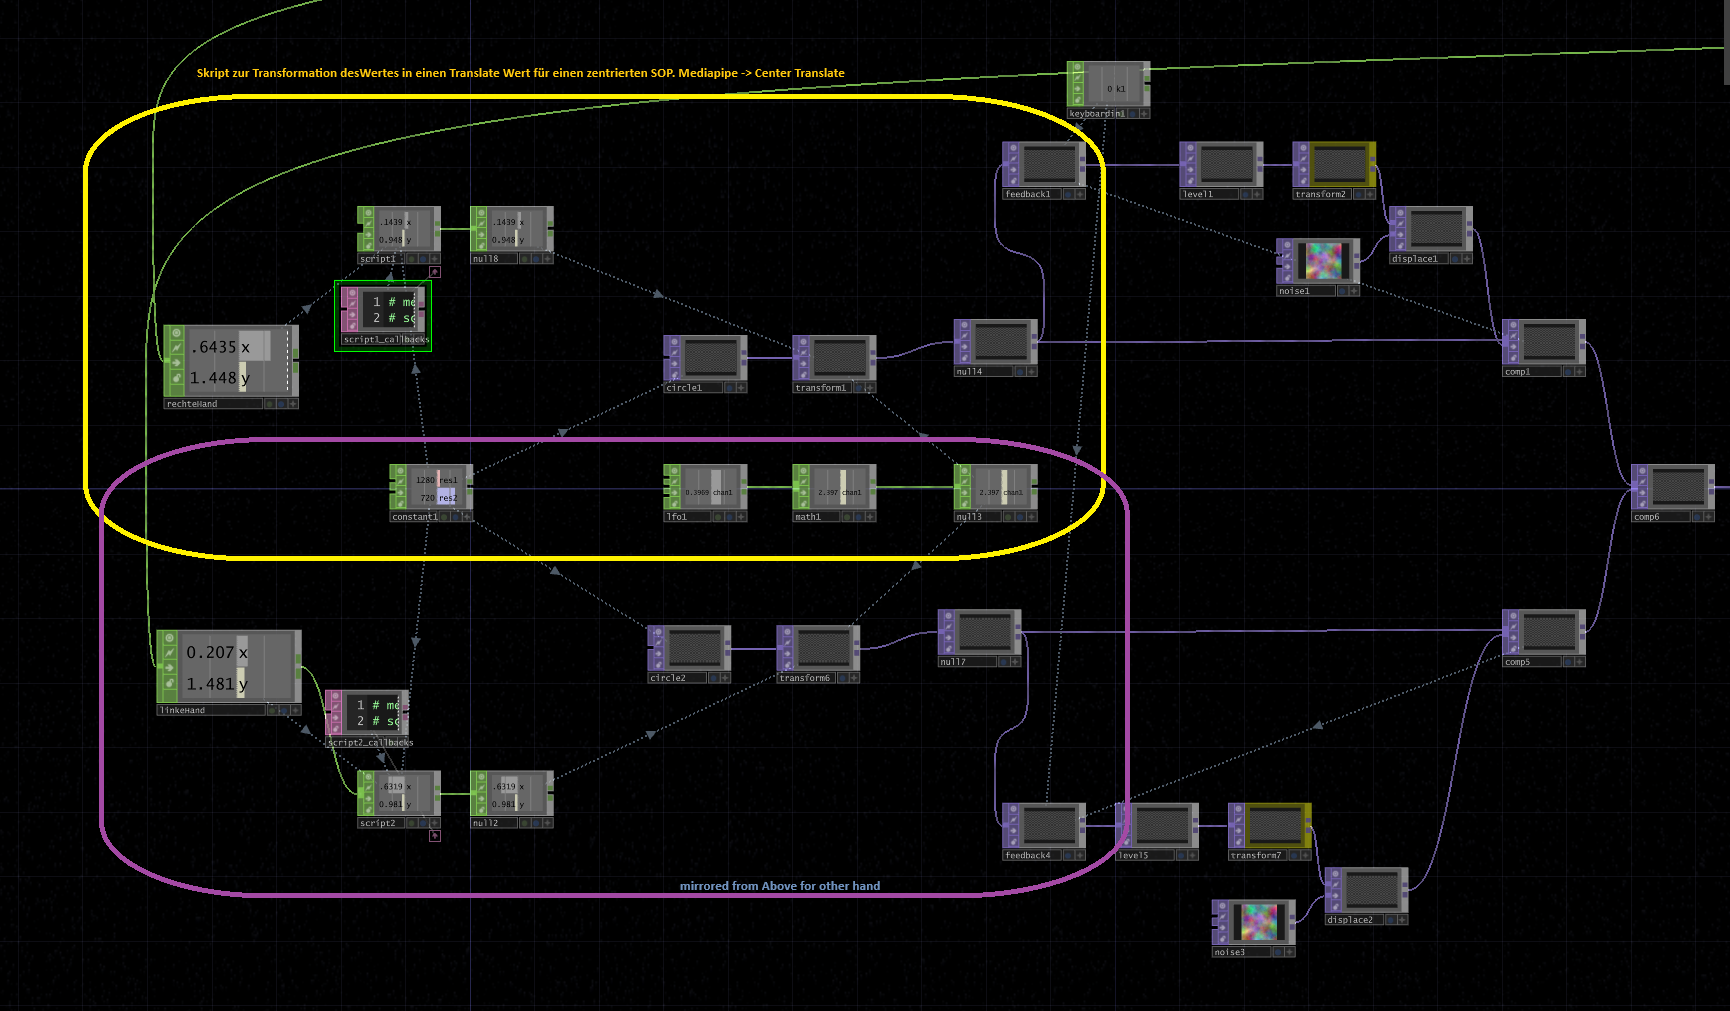
\includegraphics[width=0.6\textwidth,height=0.25\textheight,keepaspectratio]{images/docupictures/NodeXYzuSOPZentriertemTranslate.png}
    \caption{Koordinatentransformation: Node-XY zu zentralisiertem SOP-Translate}
    \label{fig:coordinate_transformation}
\end{figure}

\begin{figure}[!htbp]
    \centering
    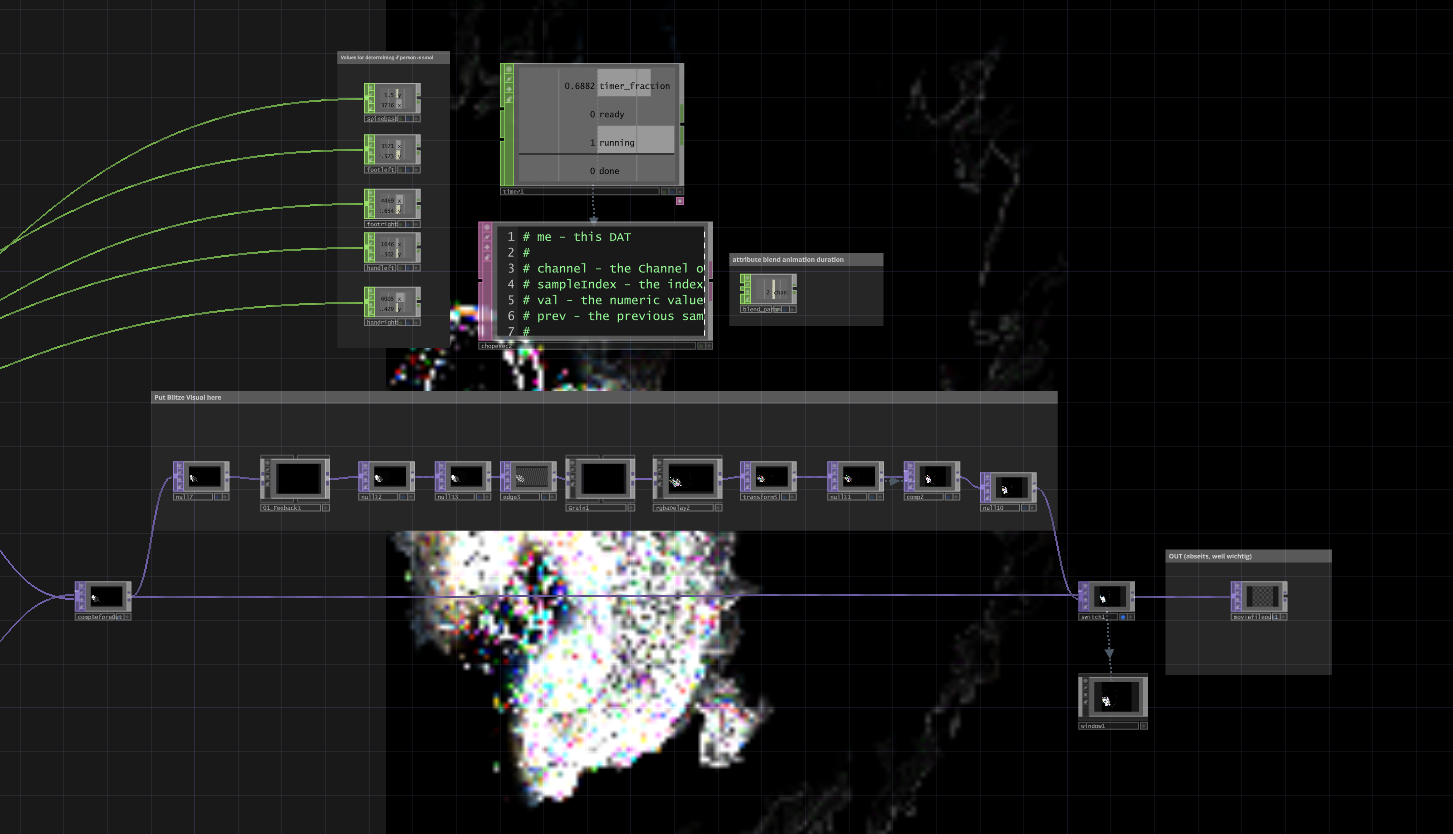
\includegraphics[width=0.6\textwidth,height=0.25\textheight,keepaspectratio]{images/docupictures/NoisyBlob_animatedSwitchzwischenBlitzUndNichtBlitzBeiTrackingTrigger.png}
    \caption{Adaptive Visual-Switch: Animierte Zustandsmaschine mit Tracking-Triggern}
    \label{fig:animated_switch}
\end{figure}

\begin{figure}[!htbp]
    \centering
    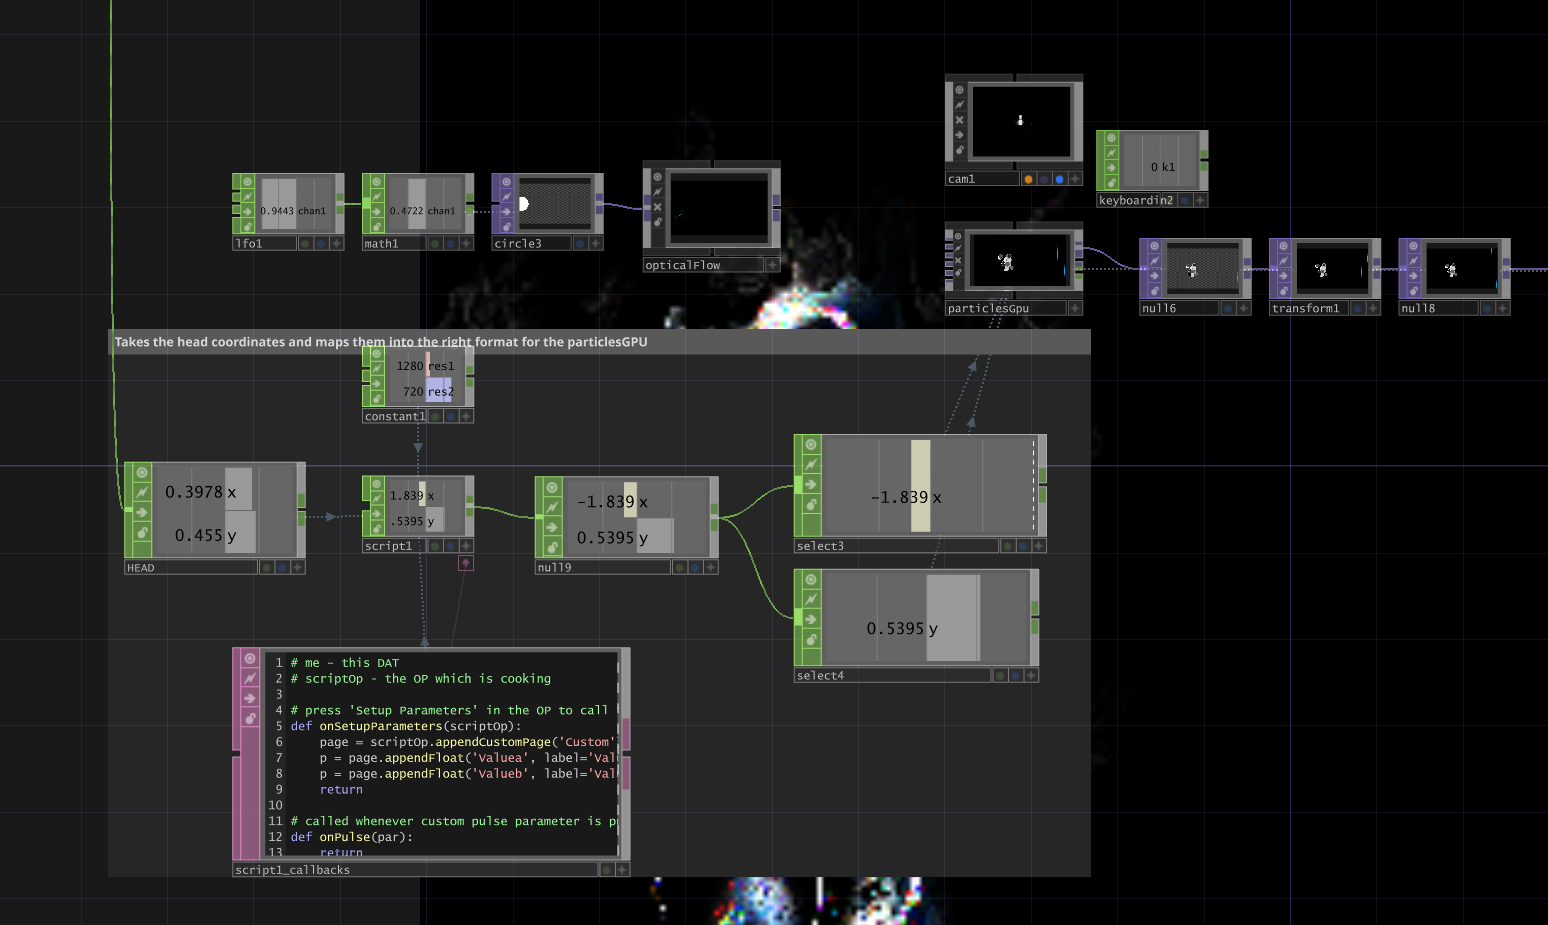
\includegraphics[width=0.6\textwidth,height=0.25\textheight,keepaspectratio]{images/docupictures/NoisyBlob_HEAD_to_ParticleGPU_Translate.png}
    \caption{ParticleGPU-Pipeline: Head-Node zu ParticleGPU Translation}
    \label{fig:particle_translation}
\end{figure}

\begin{figure}[!htbp]
    \centering
    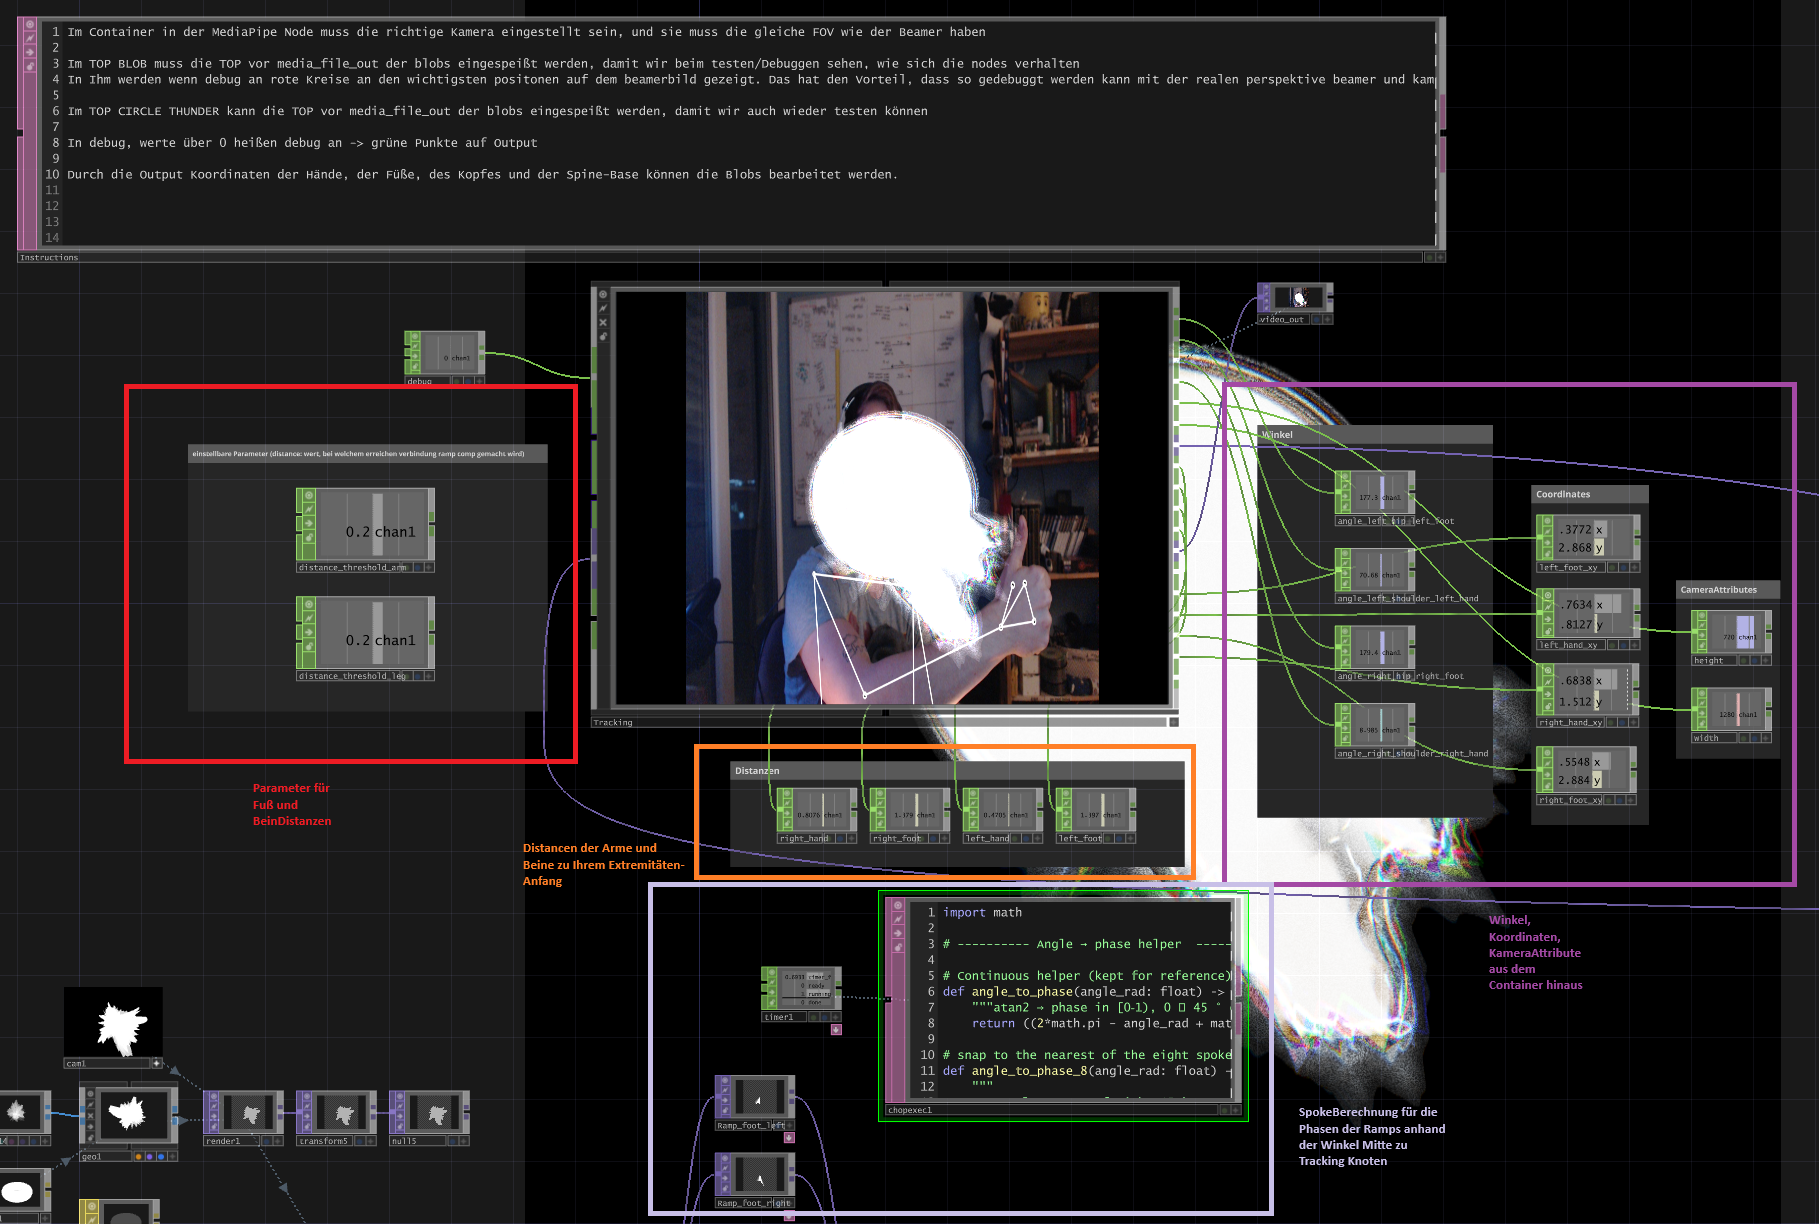
\includegraphics[width=0.6\textwidth,height=0.25\textheight,keepaspectratio]{images/docupictures/TopDown_KreisZuRampsParametisierteBerechnungen.png}
    \caption{64-Spike Radialsystem: Polar-Koordinaten-Berechnung mit parametrisierter Ramp-Generation}
    \label{fig:radial_spike_system}
\end{figure}

% Systemarchitektur und Ergebnisse figures
\begin{figure}[!htbp]
    \centering
    \includegraphics[width=0.6\textwidth,height=0.25\textheight,keepaspectratio]{images/docupictures/Finished_MediaPipeContainer_mitErkl�rungen.png}
    \caption{MediaPipe-Container: Vollst�ndige Pipeline-Architektur mit Erkl�rungen}
    \label{fig:mediapipe_architecture}
\end{figure}

\begin{figure}[!htbp]
    \centering
    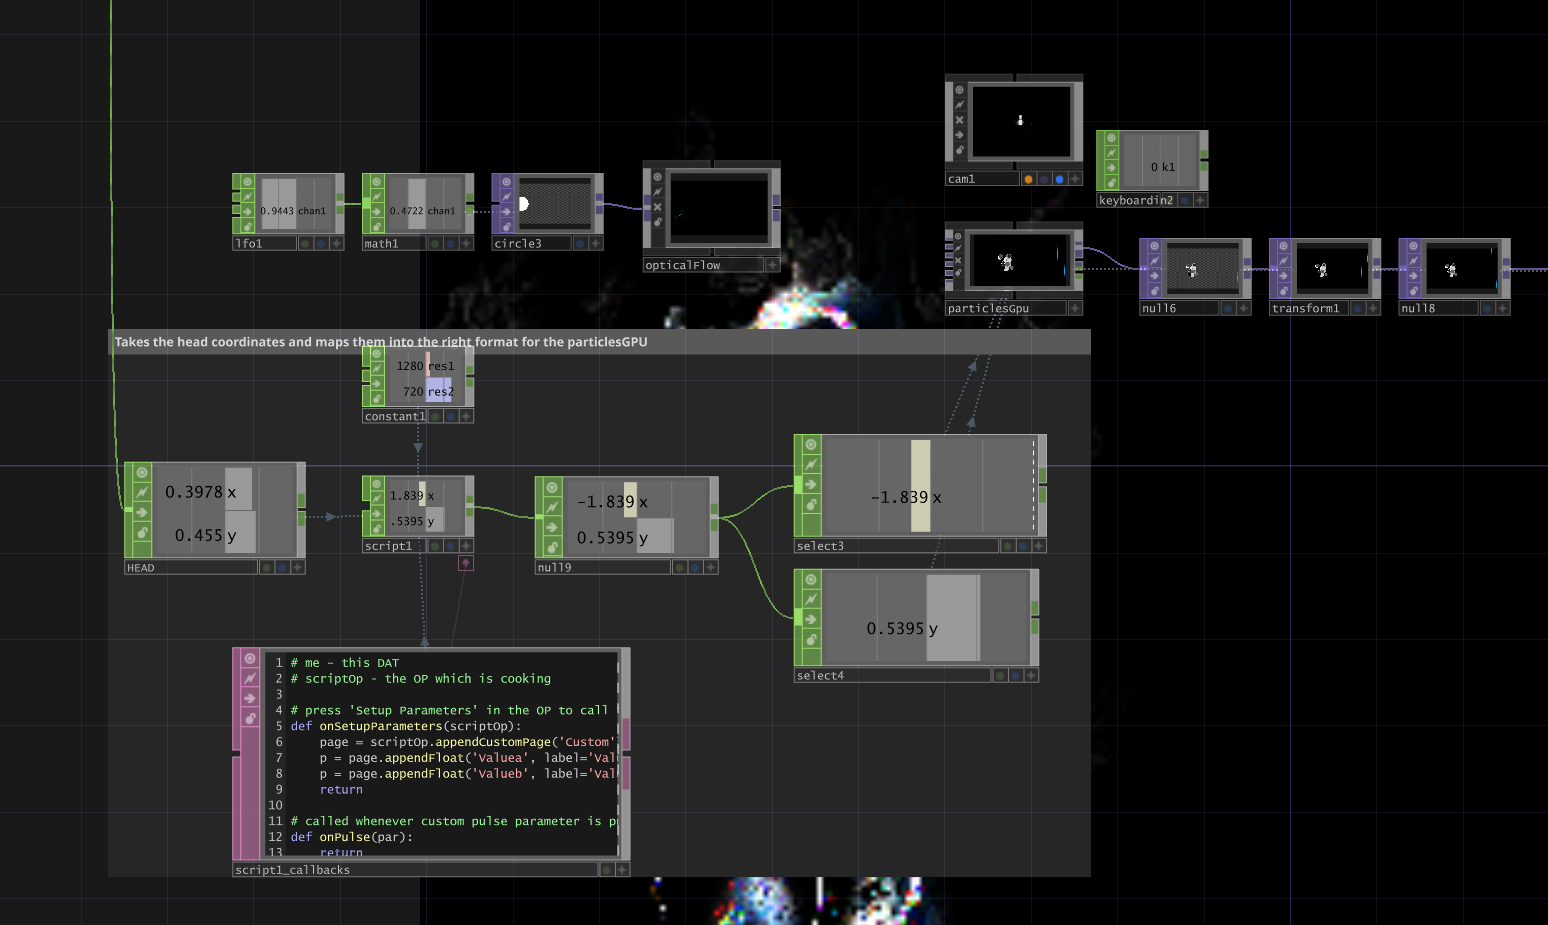
\includegraphics[width=0.6\textwidth,height=0.25\textheight,keepaspectratio]{images/docupictures/NoisyBlob_HEAD_to_ParticleGPU_Translate.png}
    \caption{Hand-Feuer-Implementation: ParticleGPU-basierte Echtzeit-Responsivit�t}
    \label{fig:hand_fire_system}
\end{figure}

\begin{figure}[!htbp]
    \centering
    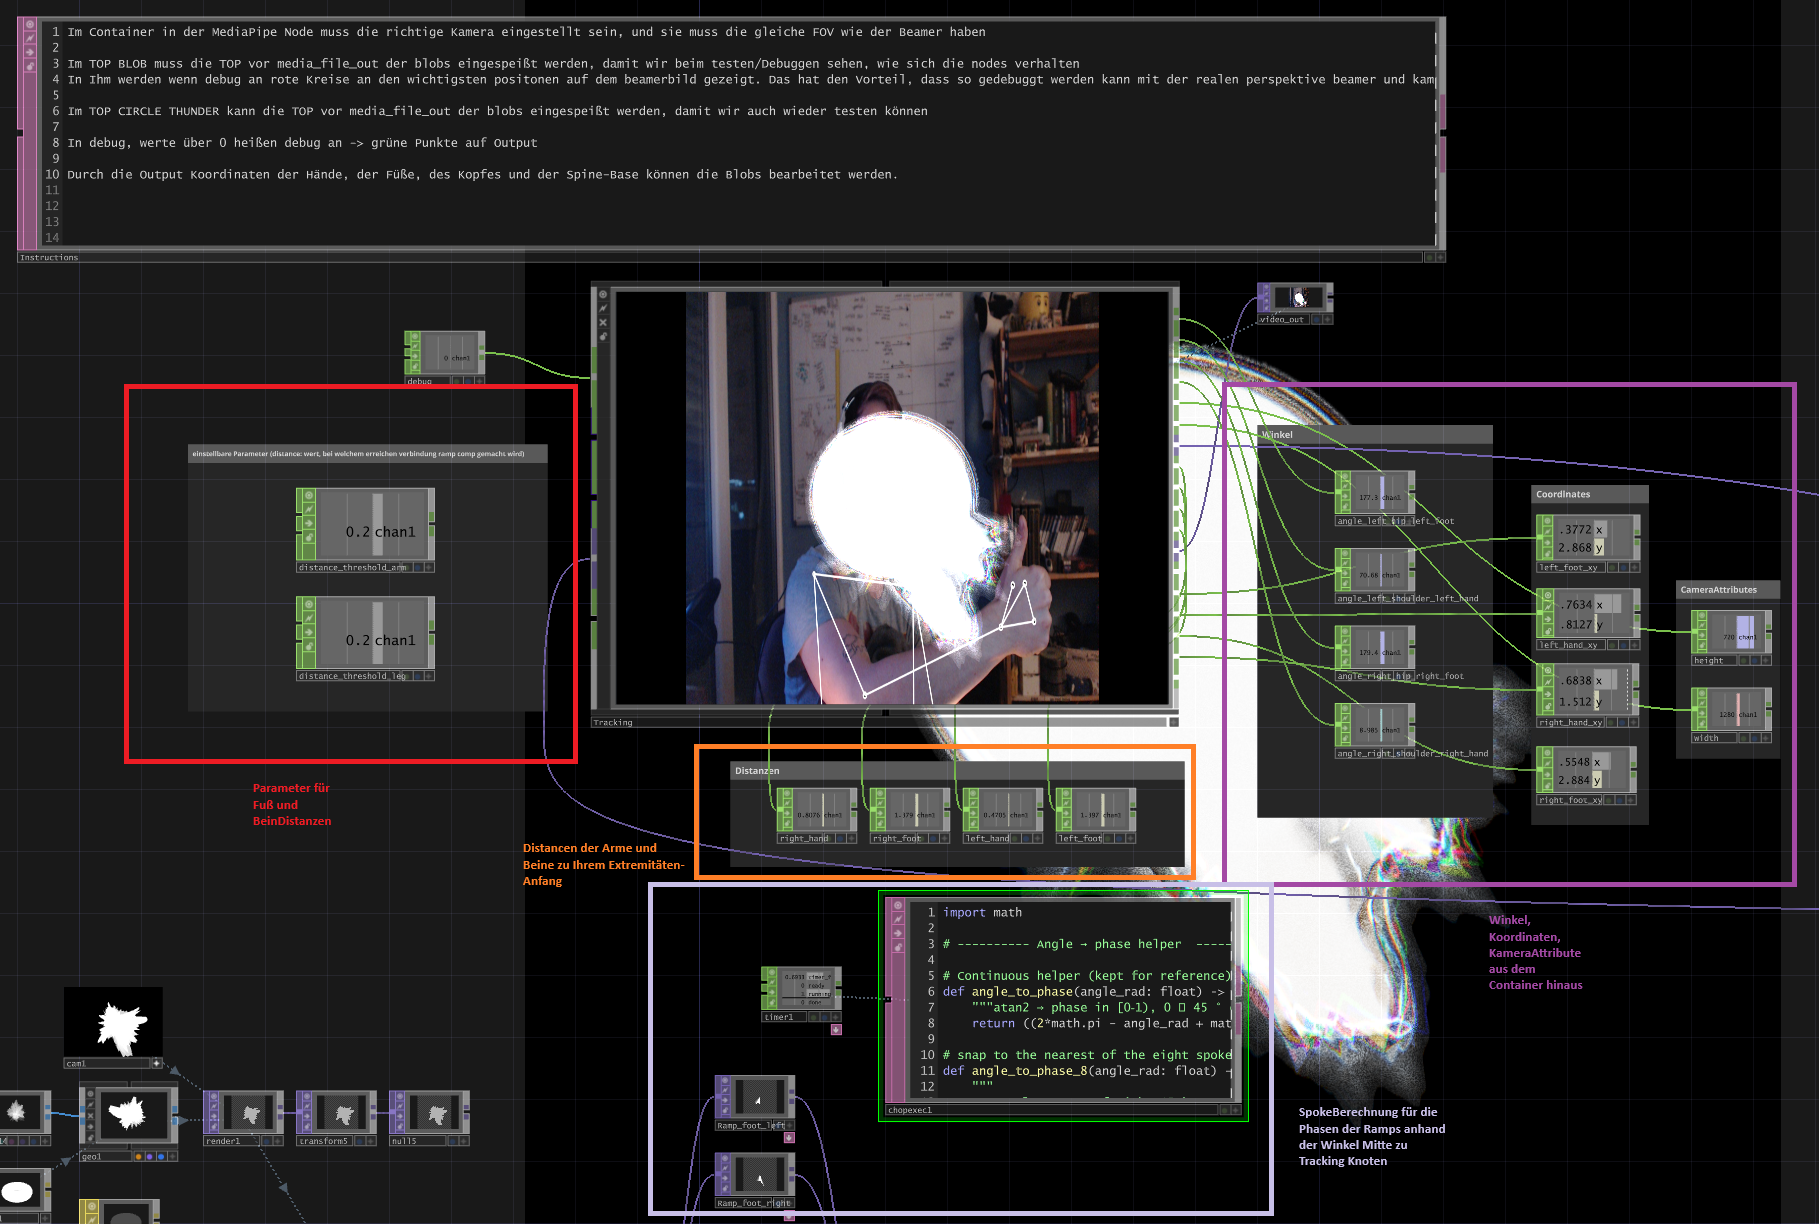
\includegraphics[width=0.6\textwidth,height=0.25\textheight,keepaspectratio]{images/docupictures/TopDown_KreisZuRampsParametisierteBerechnungen.png}
    \caption{64-Spike-System: Polar-Koordinaten-Mapping mit 5,625� Aufl�sung}
    \label{fig:spike_system_production}
\end{figure}

% Entwicklungsprozess figures
\begin{figure}[!htbp]
    \centering
    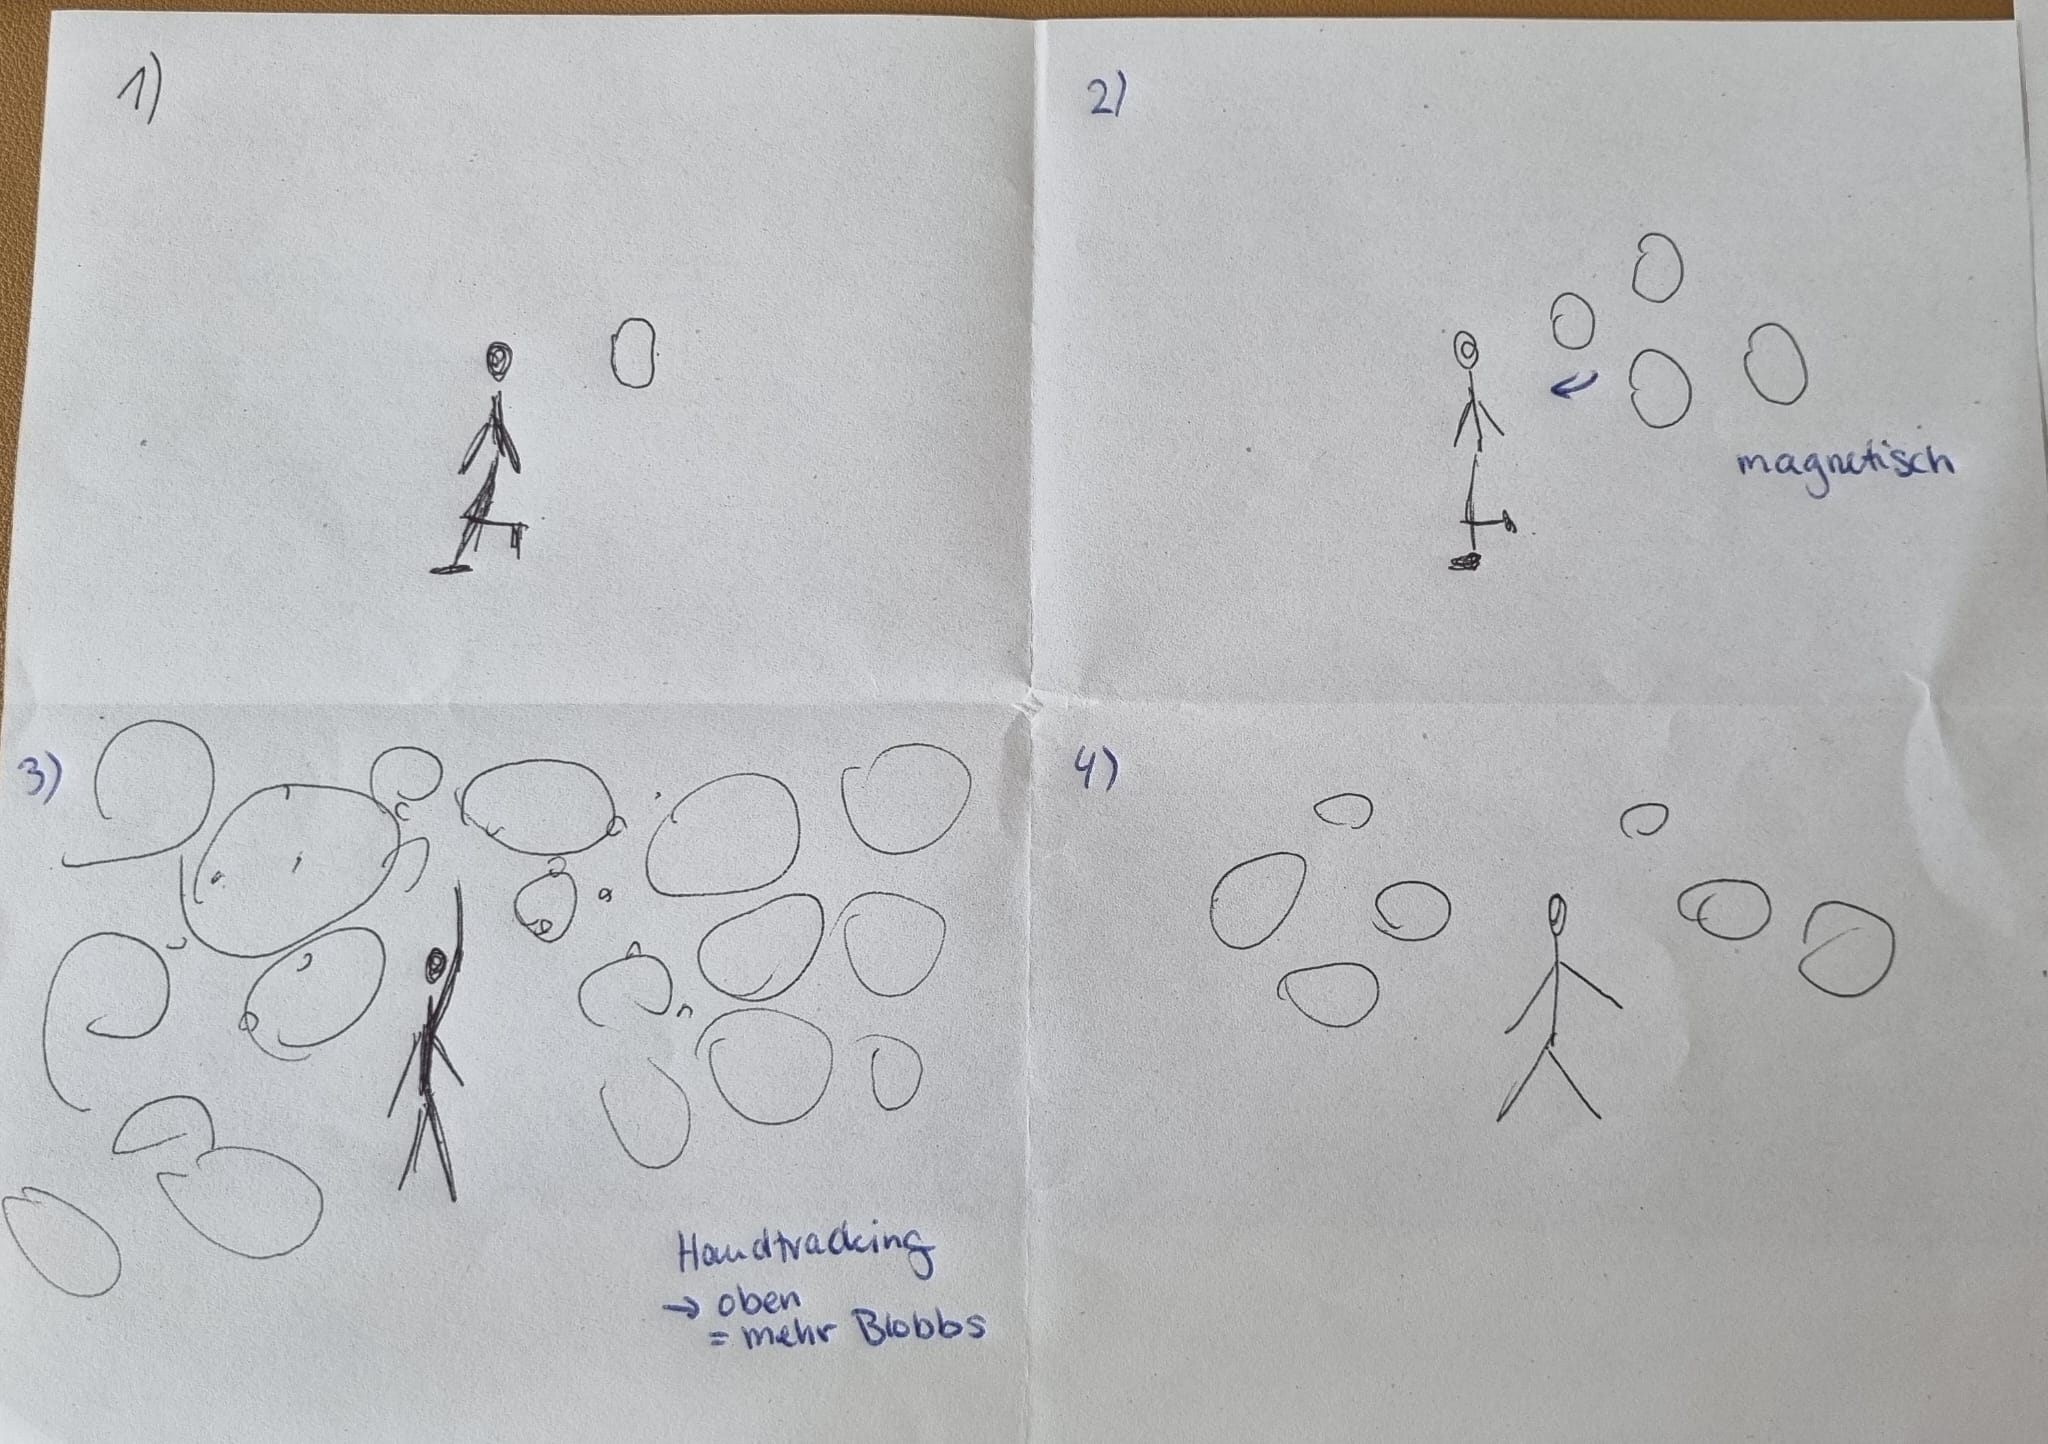
\includegraphics[width=0.6\textwidth,height=0.25\textheight,keepaspectratio]{images/Sprint3_1.jpg}
    \caption{Designkonzept: Skalierungsresponsive Visual-Transformation}
    \label{fig:design_evolution}
\end{figure}

\begin{figure}[!htbp]
    \centering
    % TODO: Replace with actual infrared pipeline diagram
    % \includegraphics[width=0.6\textwidth,height=0.25\textheight,keepaspectratio]{images/infrared_pipeline_diagram.png}
    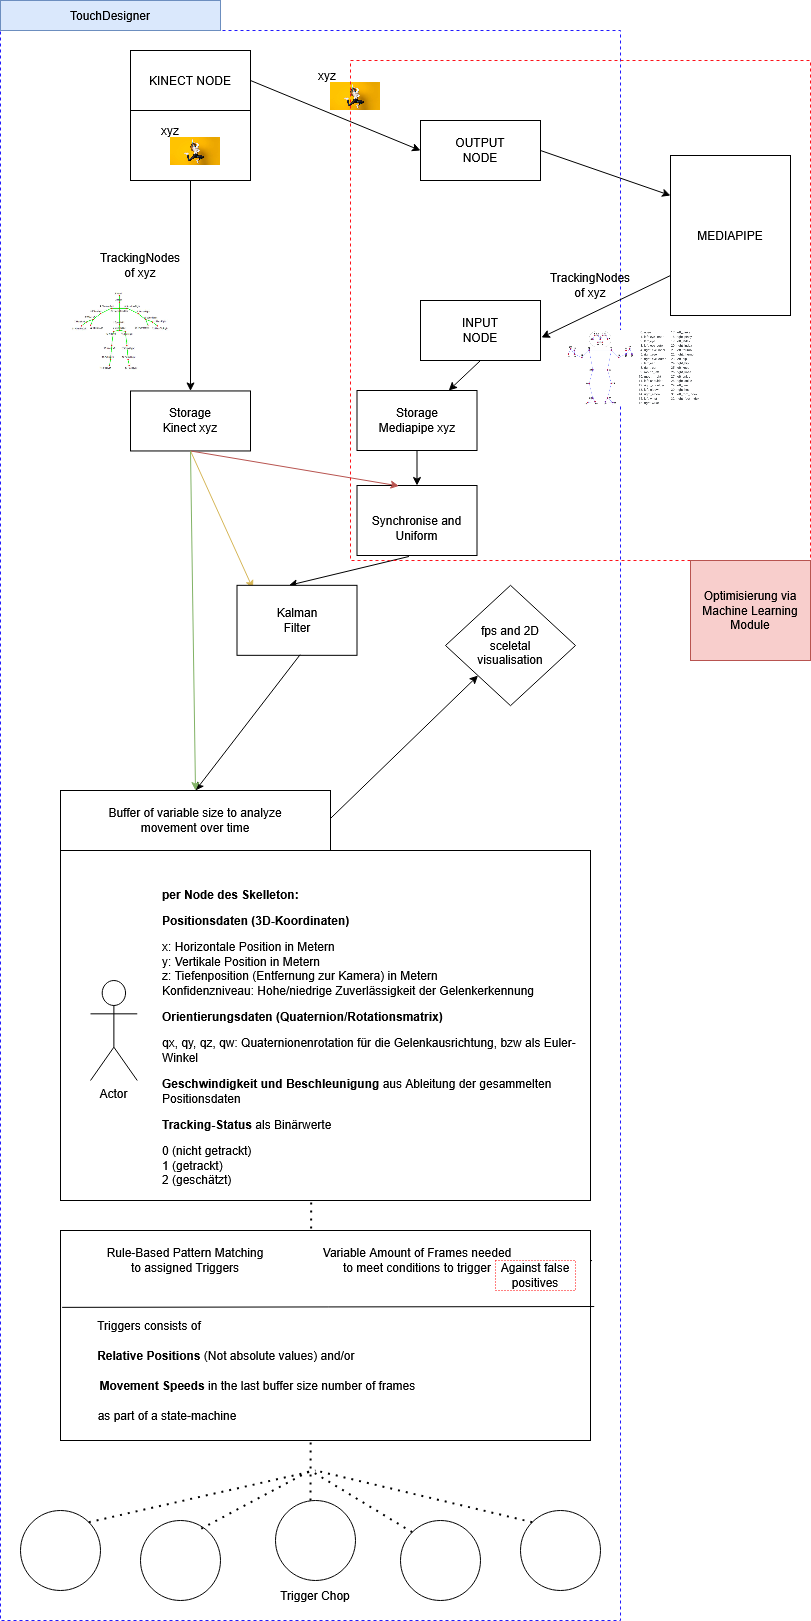
\includegraphics[width=0.6\textwidth,height=0.25\textheight,keepaspectratio]{images/MASK.png}
    \caption{Infrarot-MediaPipe-Pipeline: Technische L�sung f�r Produktionsumgebungen (Platzhalter - spezifisches Infrarot-Pipeline-Diagramm erforderlich)}
    \label{fig:infrared_solution}
\end{figure}

% Demonstration figures
\begin{figure}[!htbp]
    \centering
    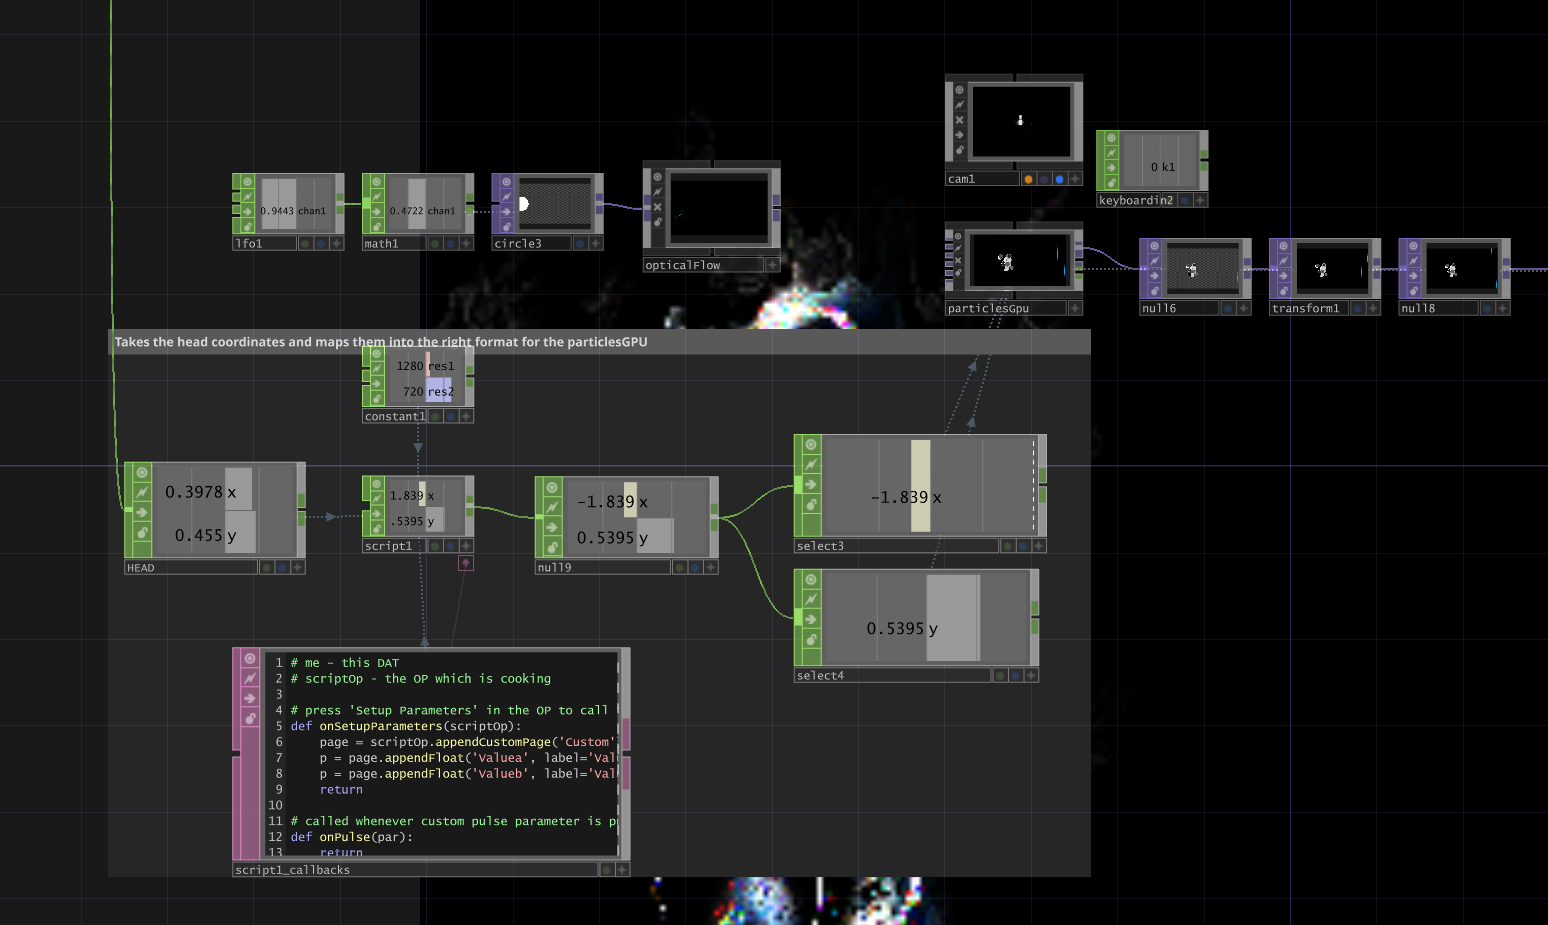
\includegraphics[width=0.6\textwidth,height=0.25\textheight,keepaspectratio]{images/docupictures/NoisyBlob_HEAD_to_ParticleGPU_Translate.png}
    \caption{Hand-Feuer-Effekte: Blaue Partikel folgen Handbewegungen in Echtzeit}
    \label{fig:particle_hands}
\end{figure}

\begin{figure}[!htbp]
    \centering
    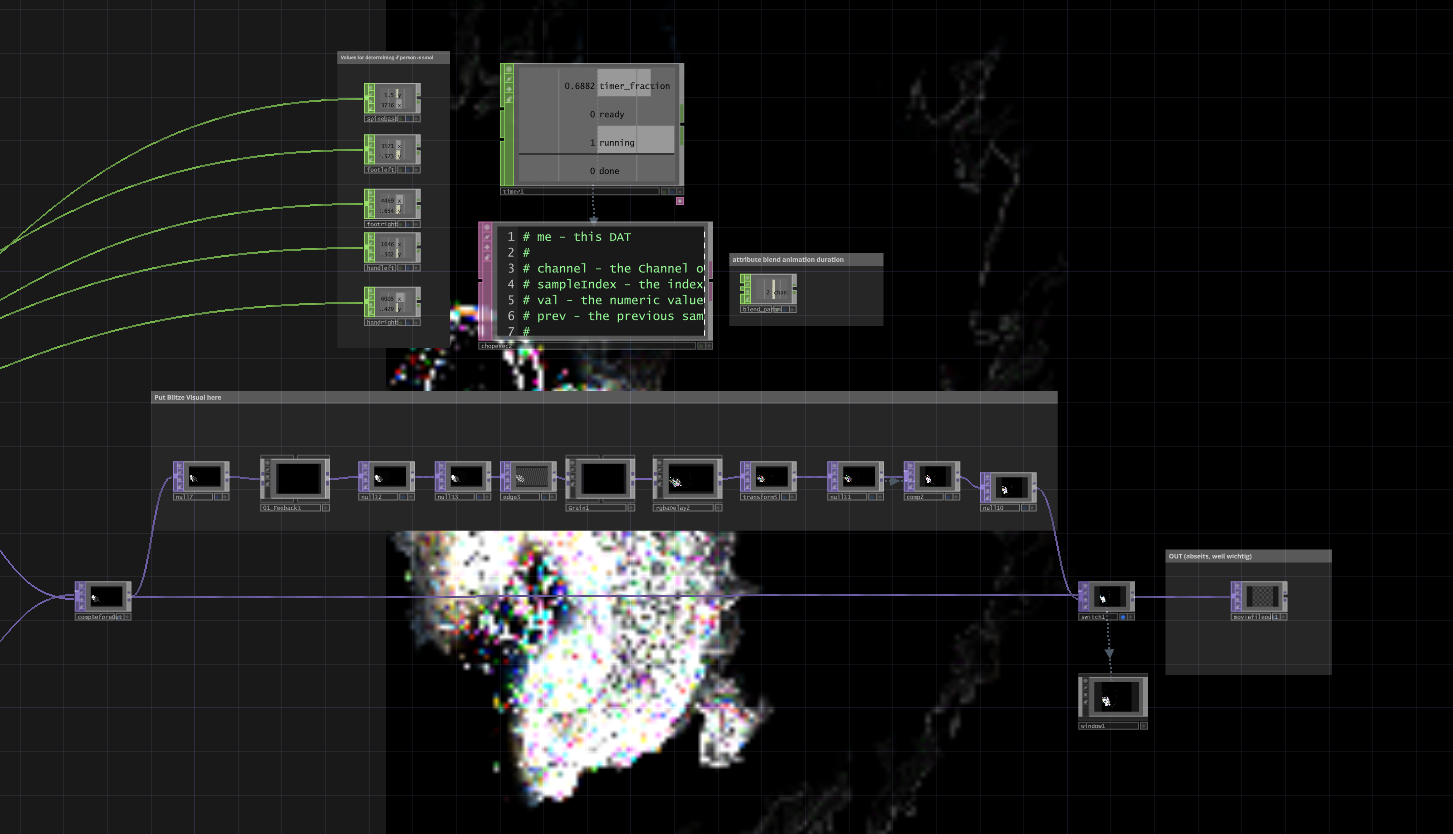
\includegraphics[width=0.6\textwidth,height=0.25\textheight,keepaspectratio]{images/docupictures/NoisyBlob_animatedSwitchzwischenBlitzUndNichtBlitzBeiTrackingTrigger.png}
    \caption{Adaptive Kopfpartikel: Zustandswechsel basierend auf Handposition relativ zur Schulter}
    \label{fig:relative_switch}
\end{figure}

\begin{figure}[!htbp]
    \centering
    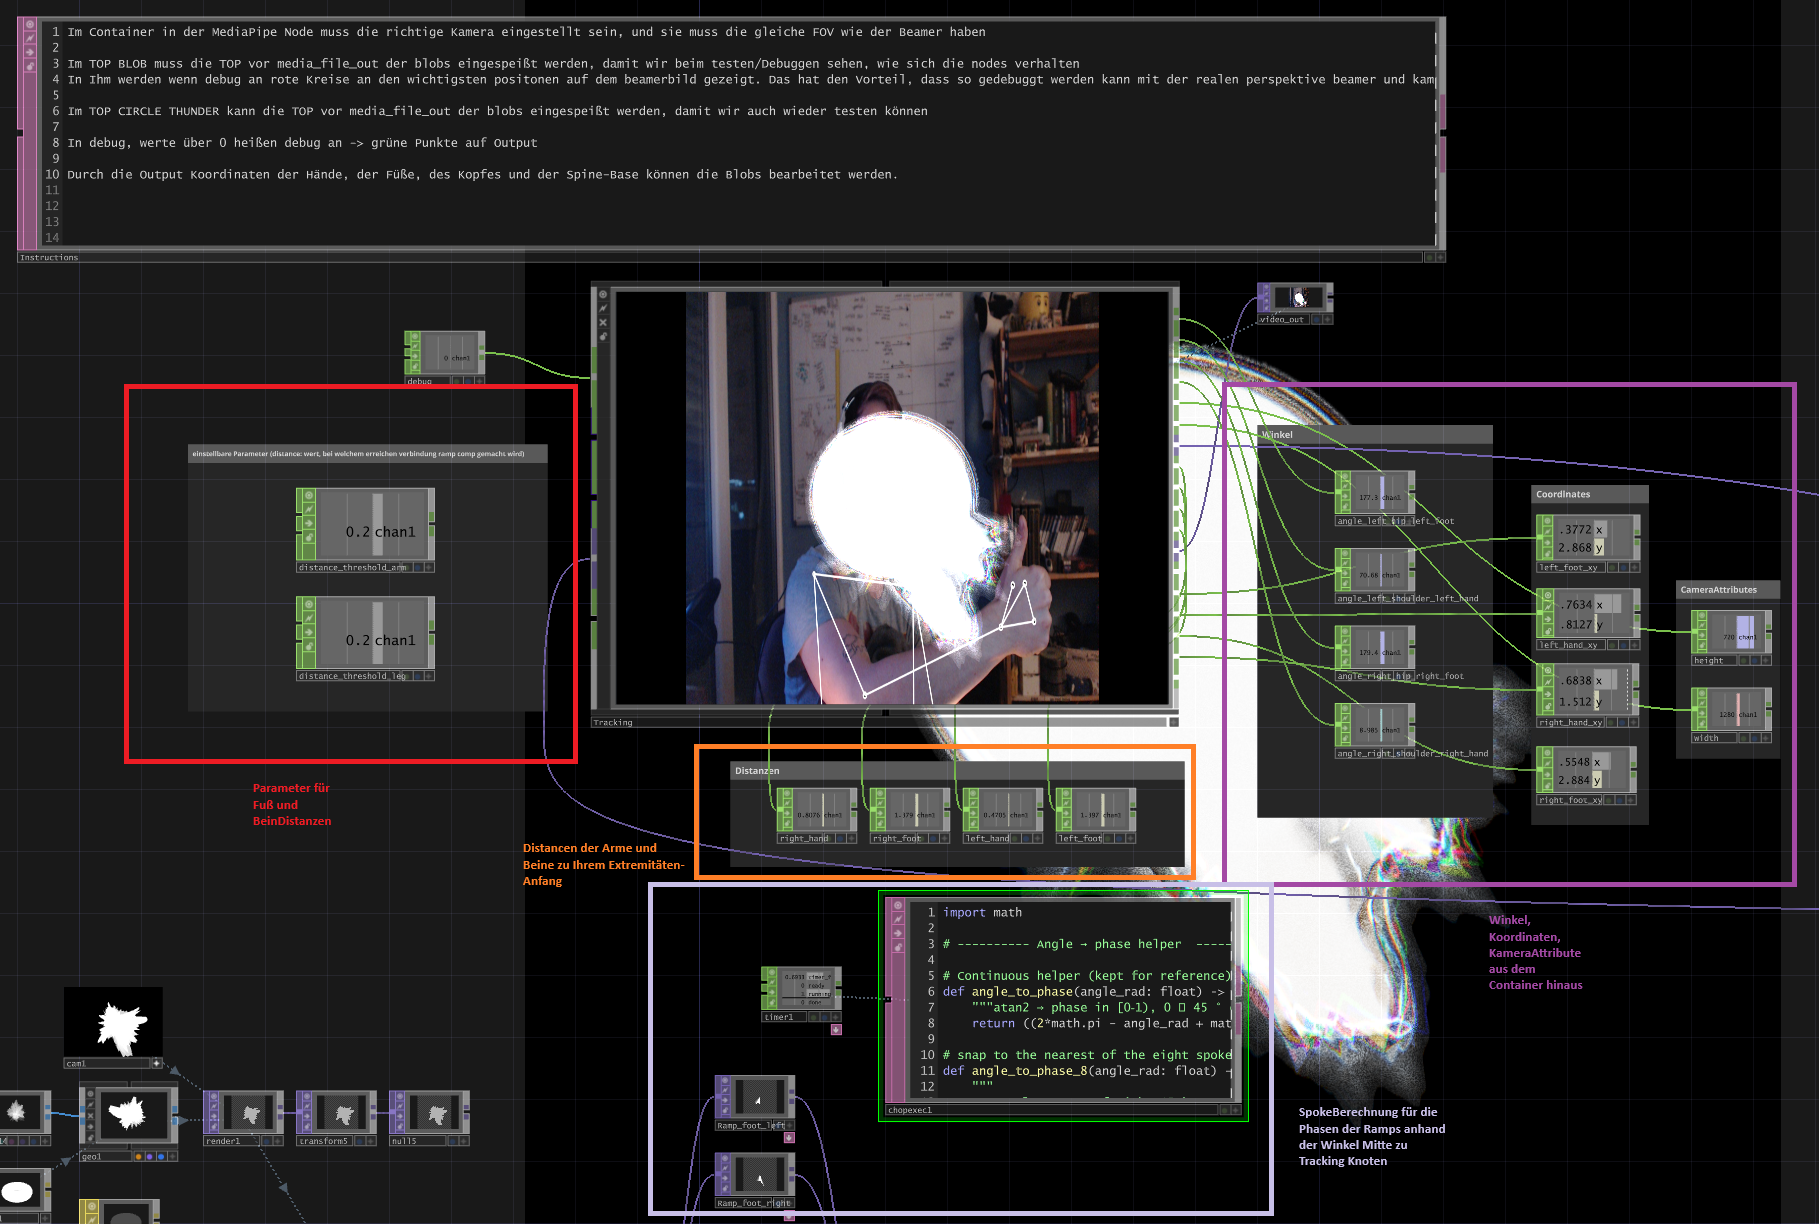
\includegraphics[width=0.6\textwidth,height=0.25\textheight,keepaspectratio]{images/docupictures/TopDown_KreisZuRampsParametisierteBerechnungen.png}
    \caption{64-Spike Radialsystem: Winkelaufl�sung von 5,625� f�r pr�zise Extremit�tenerkennung}
    \label{fig:spike_system}
\end{figure}

\begin{figure}[!htbp]
    \centering
    \includegraphics[width=0.6\textwidth,height=0.25\textheight,keepaspectratio]{images/docupictures/Finished_MediaPipeContainer_mitErkl�rungen.png}
    \caption{Debug-Visualisierung: MediaPipe-Skelett-Erkennung im Infrarot-Modus}
    \label{fig:debug_circles}
\end{figure}

\begin{figure}[!htbp]
    \centering
    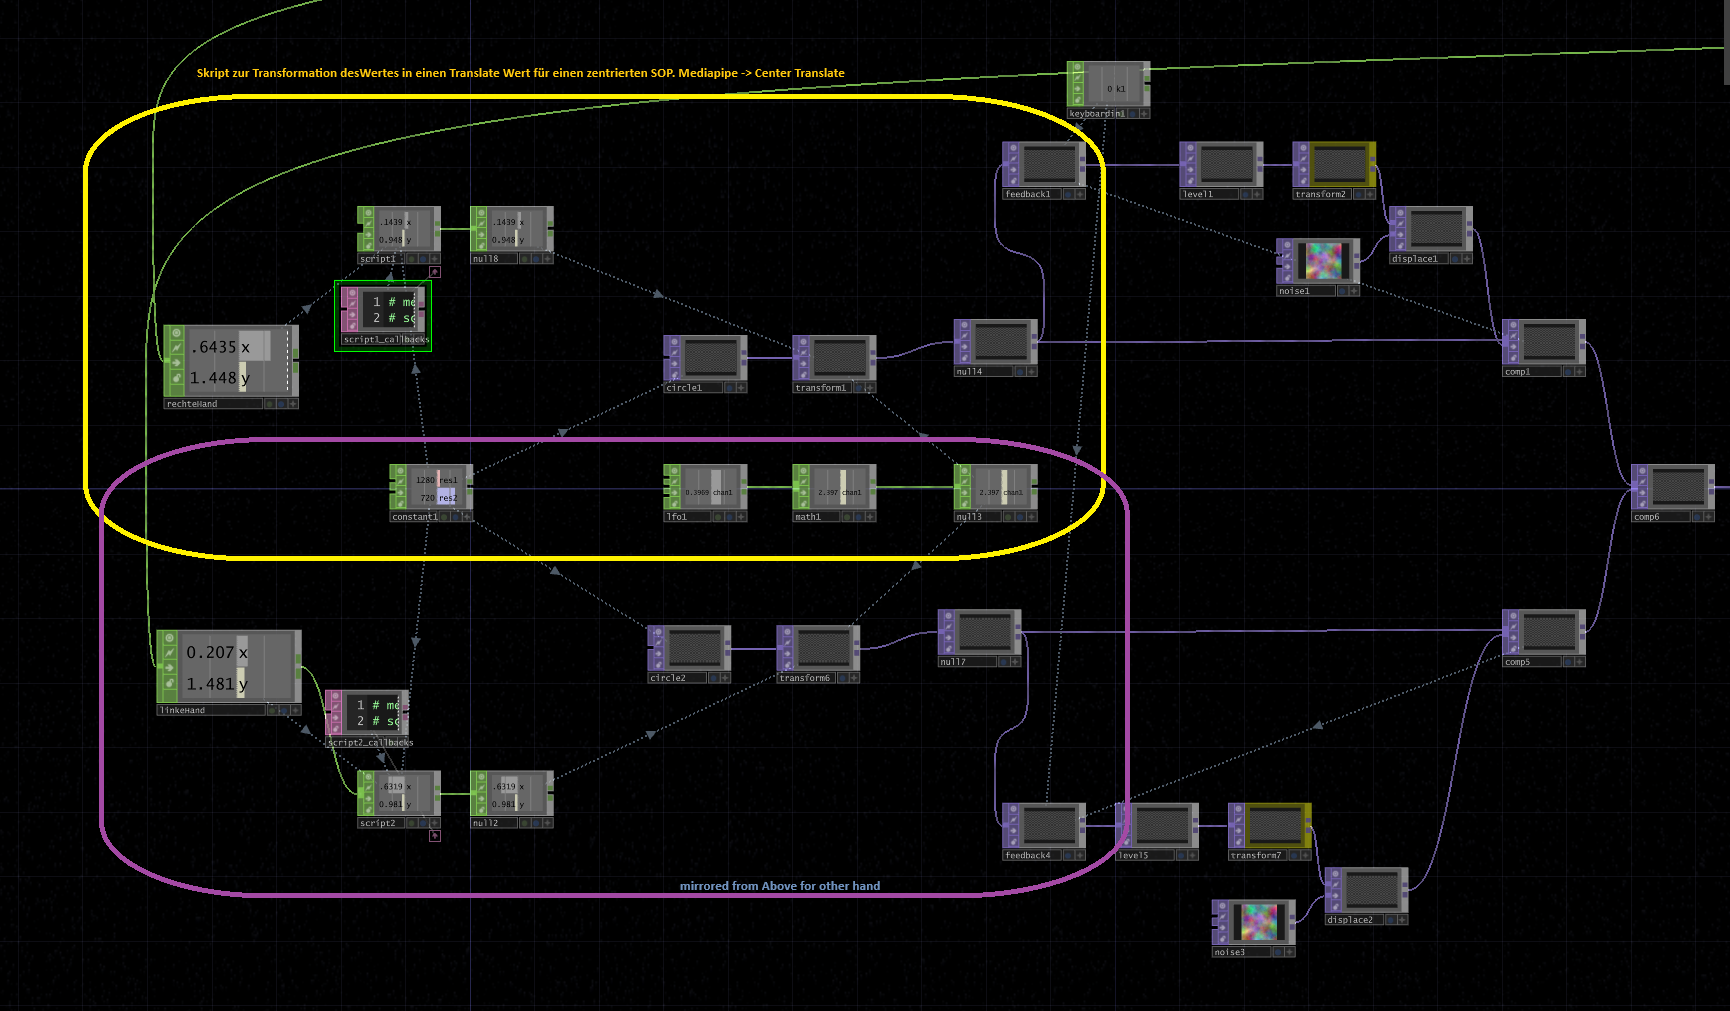
\includegraphics[width=0.6\textwidth,height=0.25\textheight,keepaspectratio]{images/docupictures/NodeXYzuSOPZentriertemTranslate.png}
    \caption{Koordinatentransformation: MediaPipe-Normalisierung zu TouchDesigner-Weltkoordinaten}
    \label{fig:coordinate_transform}
\end{figure}

\begin{figure}[!htbp]
    \centering
    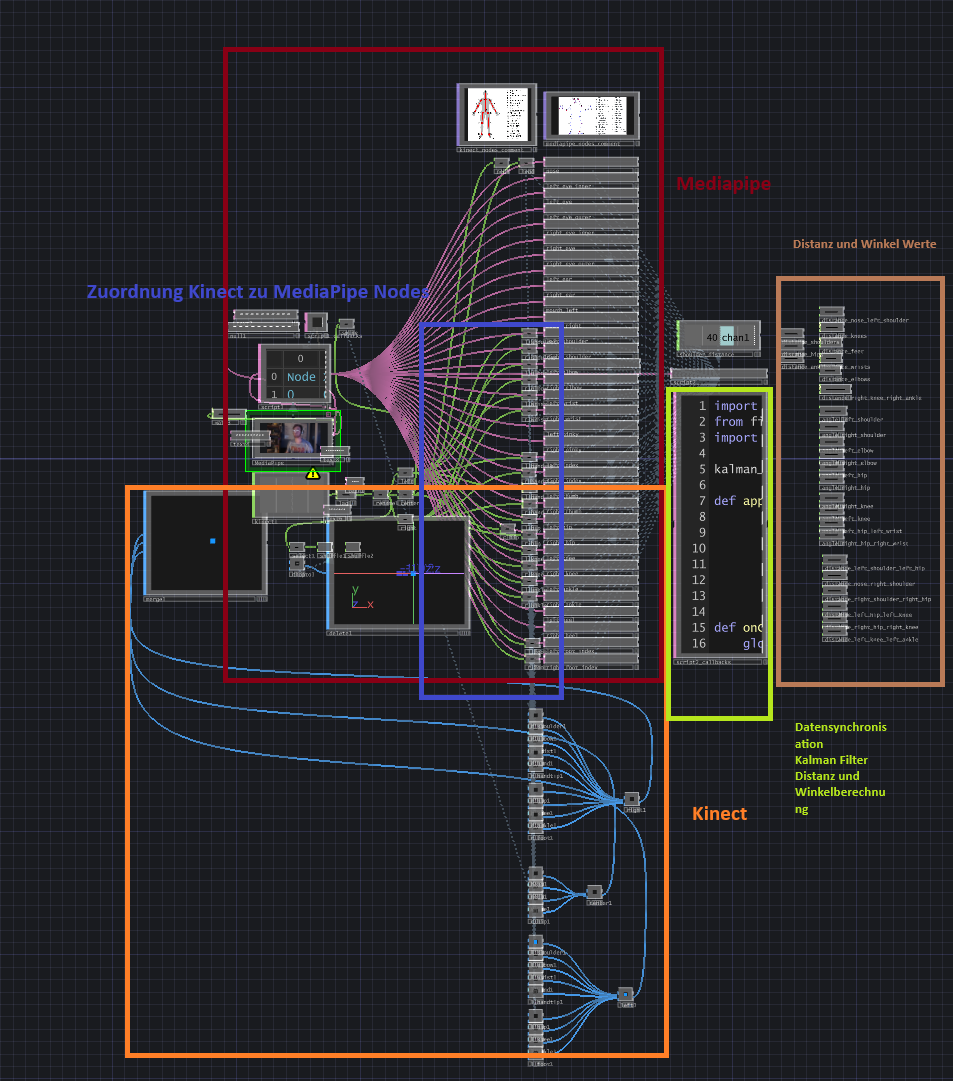
\includegraphics[width=0.6\textwidth,height=0.25\textheight,keepaspectratio]{images/docupictures/KinectMediaPipe_Testing.png}
    \caption{Geometrische Analyse: Echtzeit-Berechnung von Skelett-Relationen}
    \label{fig:distance_angle}
\end{figure}

% Ausf�hrungsdokumentation figures
\begin{figure}[!htbp]
   \centering
   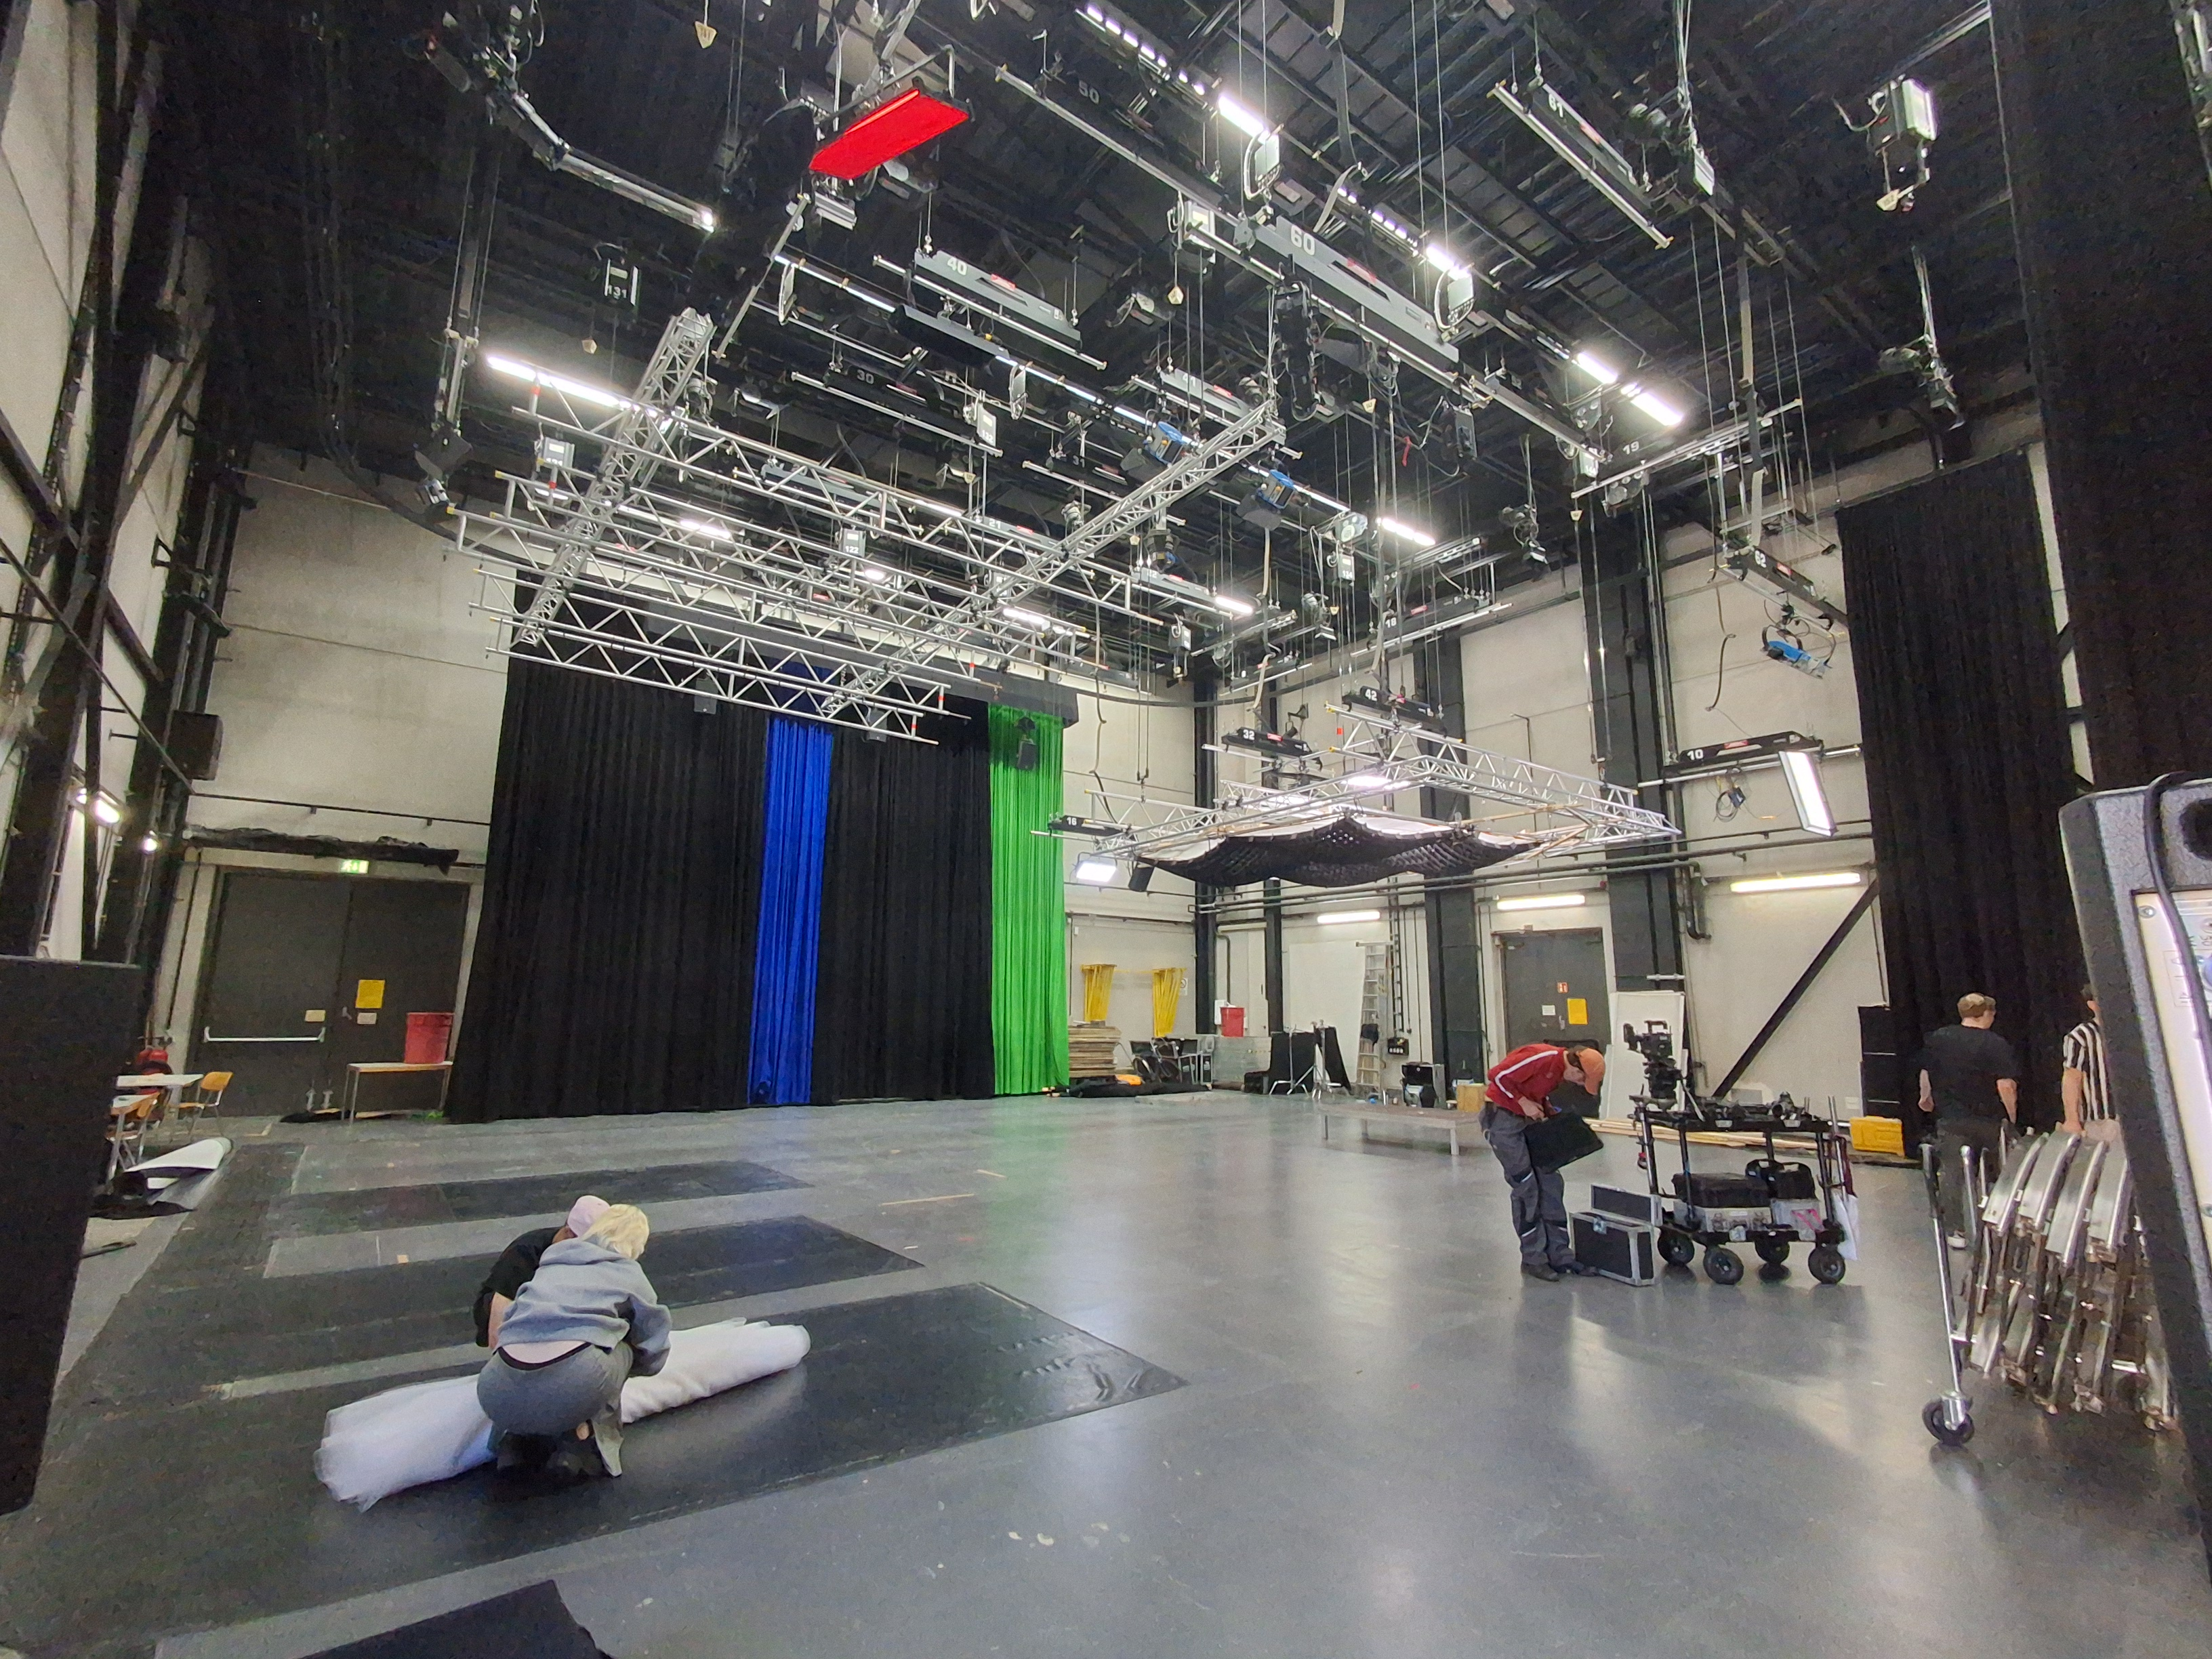
\includegraphics[width=0.6\textwidth,height=0.25\textheight,keepaspectratio]{images/onSetImages/InsideWideshotAlbrechtAdeStudio.jpg}
   \caption{Albrecht-Ade-Studio: Erste Eindr�cke der gro�en Soundstage vor Produktionsbeginn}
   \label{fig:studio_interior}
\end{figure}

\begin{figure}[!htbp]
   \centering
   \includegraphics[width=0.6\textwidth,height=0.25\textheight,keepaspectratio]{images/onSetImages/MartyBehindTheStudioCurtainDoingTouchDesigner.jpg}
   \caption{Technische Umsetzung: TouchDesigner-Bedienung hinter dem Studievorhang w�hrend der Produktion}
   \label{fig:technical_operation}
\end{figure}

\begin{figure}[!htbp]
   \centering
   \includegraphics[width=0.6\textwidth,height=0.25\textheight,keepaspectratio]{images/onSetImages/wideStudioShotPreparingTopDownSpikeShot.jpg}
   \caption{Studio-Vorbereitung: Setup f�r Top-Down-Spike-System mit Overhead-Kamera-Positionierung}
   \label{fig:topdown_setup}
\end{figure}

\begin{figure}[!htbp]
   \centering
   \includegraphics[width=0.6\textwidth,height=0.25\textheight,keepaspectratio]{images/onSetImages/cameraBTSPicofACameraScreenOfTopDown64SpikeOfDancerOnFloor.jpg}
   \caption{Kameramonitor: Top-Down-Aufnahme des 64-Spike-Systems mit T�nzer auf dem Studioboden}
   \label{fig:camera_monitor}
\end{figure}

\begin{figure}[!htbp]
   \centering
   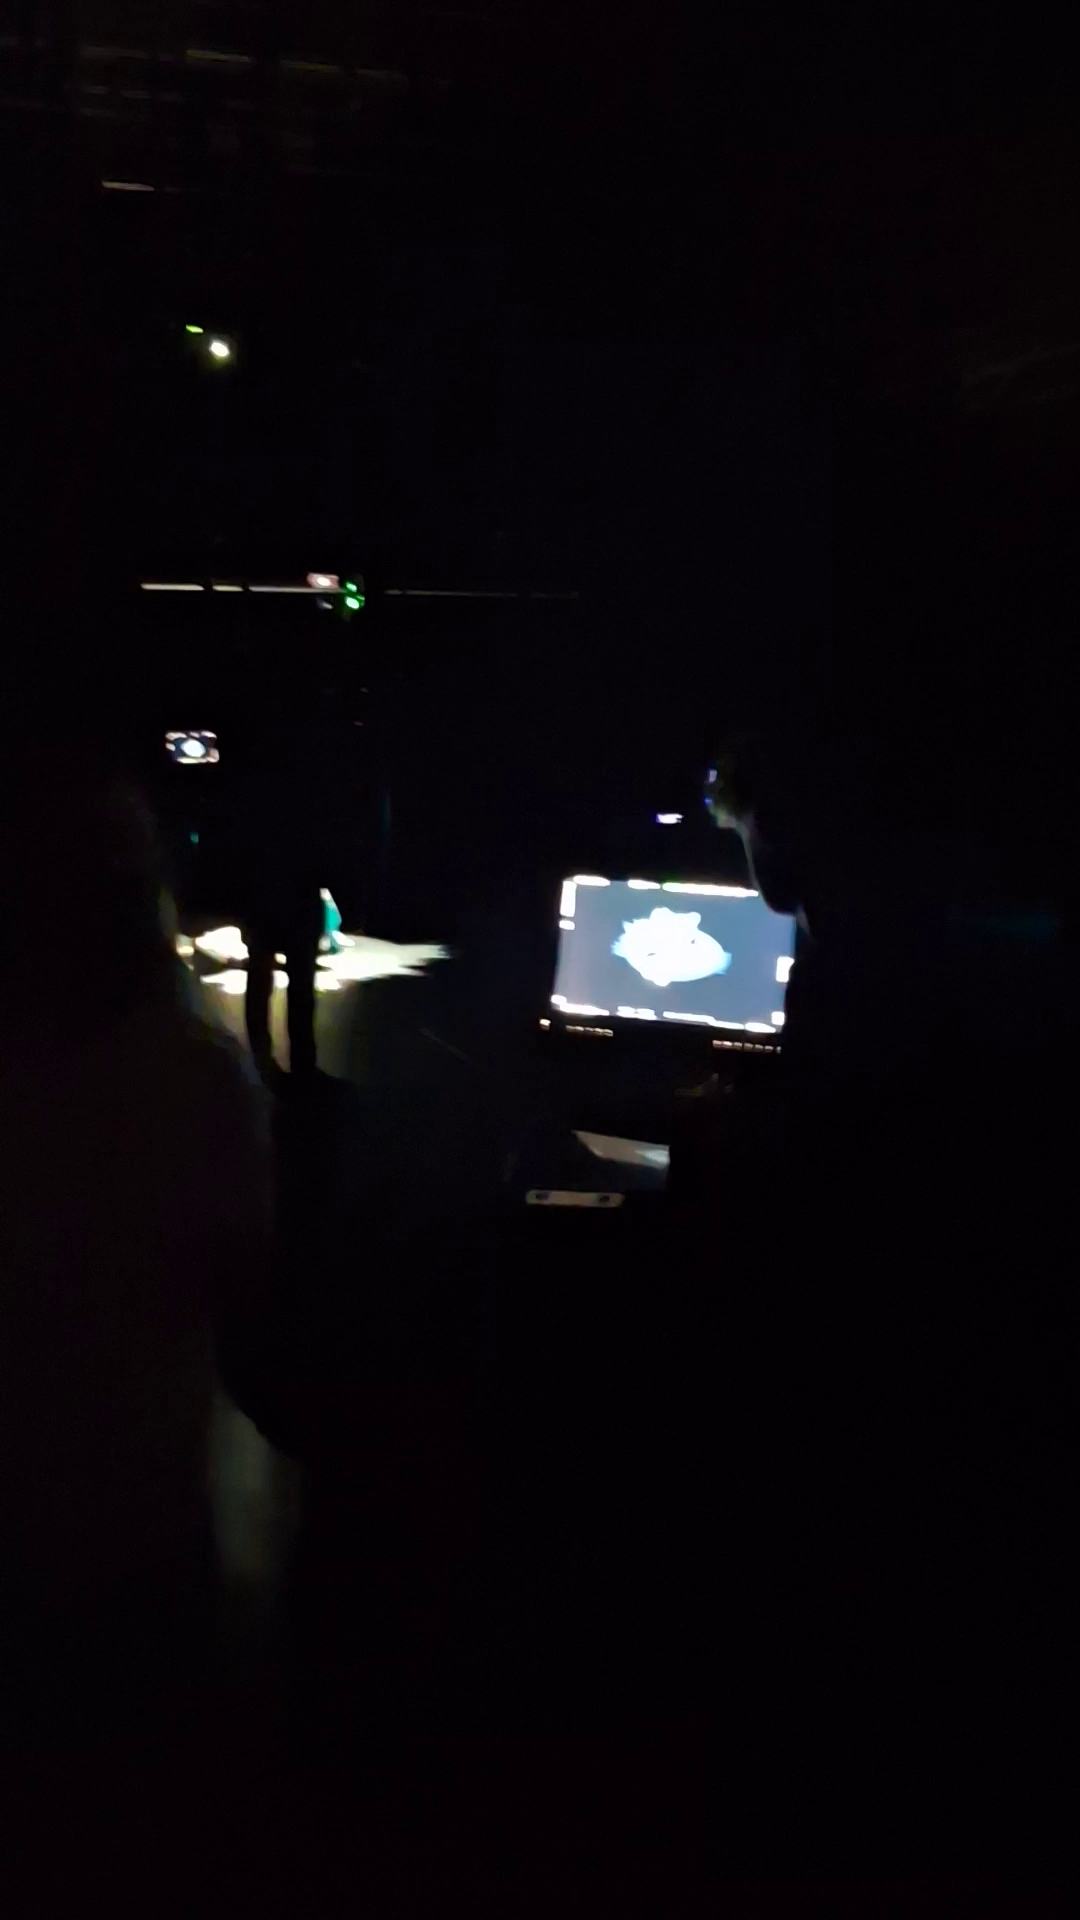
\includegraphics[width=0.6\textwidth,height=0.25\textheight,keepaspectratio]{images/BTS_ProducerScreen.png}
   \caption{Spike-System in Aktion: Reagiert pr�zise auf Hand- und Fu�bewegungen}
   \label{fig:spike_action}
\end{figure}

\begin{figure}[!htbp]
   \centering
   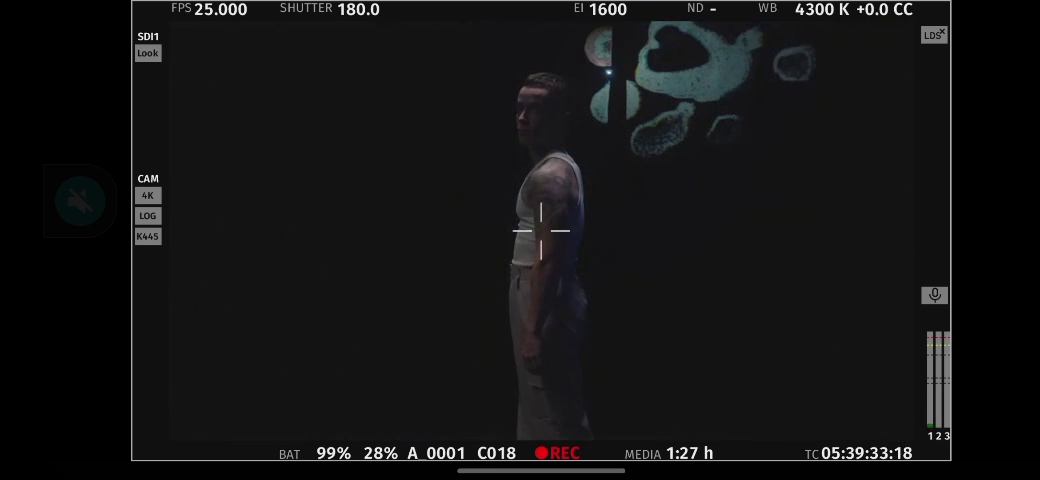
\includegraphics[width=0.6\textwidth,height=0.25\textheight,keepaspectratio]{images/HeadTracking_HQCamera.png}
   \caption{Kopfpartikel-Setup: Komplexe Kamera-Beamer-Ausrichtung}
   \label{fig:head_setup}
\end{figure}

\begin{figure}[!htbp]
   \centering
   \includegraphics[width=0.6\textwidth,height=0.25\textheight,keepaspectratio]{images/onSetImages/PictureOfDancerBTSinSetupForHeadTrackingBubbles.jpg}
   \caption{Kopfpartikel-Setup: T�nzer bei Vorbereitung f�r Head-Tracking mit kritischen Lichtbedingungen}
   \label{fig:dancer_head_tracking}
\end{figure}

\begin{figure}[!htbp]
   \centering
   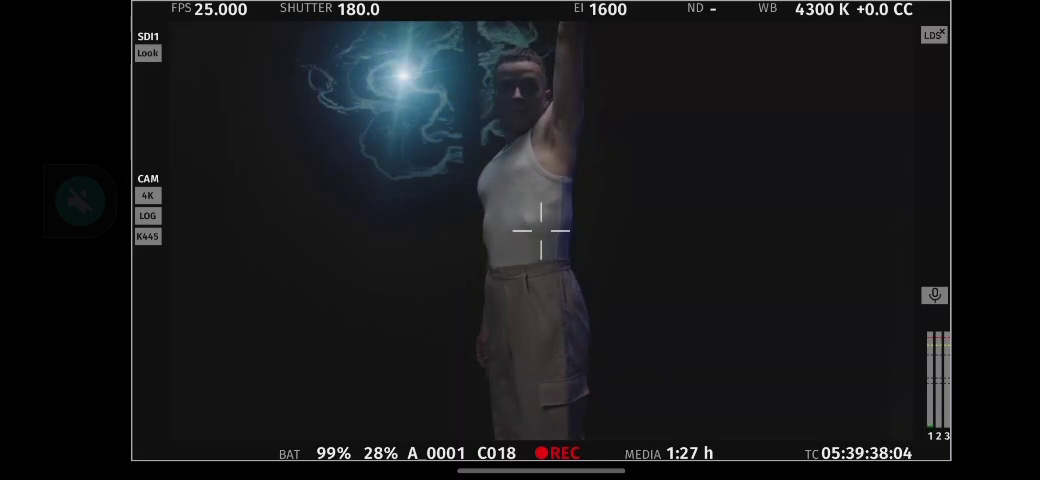
\includegraphics[width=0.6\textwidth,height=0.25\textheight,keepaspectratio]{images/HeadTrackingLeftSideOfHeadWithHeadClearlyAttached.png}
   \caption{Head-Tracking Perspektive: MediaPipe-Skelett-Erkennung aus seitlichem Blickwinkel}
   \label{fig:low_light_tracking}
\end{figure}

\begin{figure}[!htbp]
   \centering
   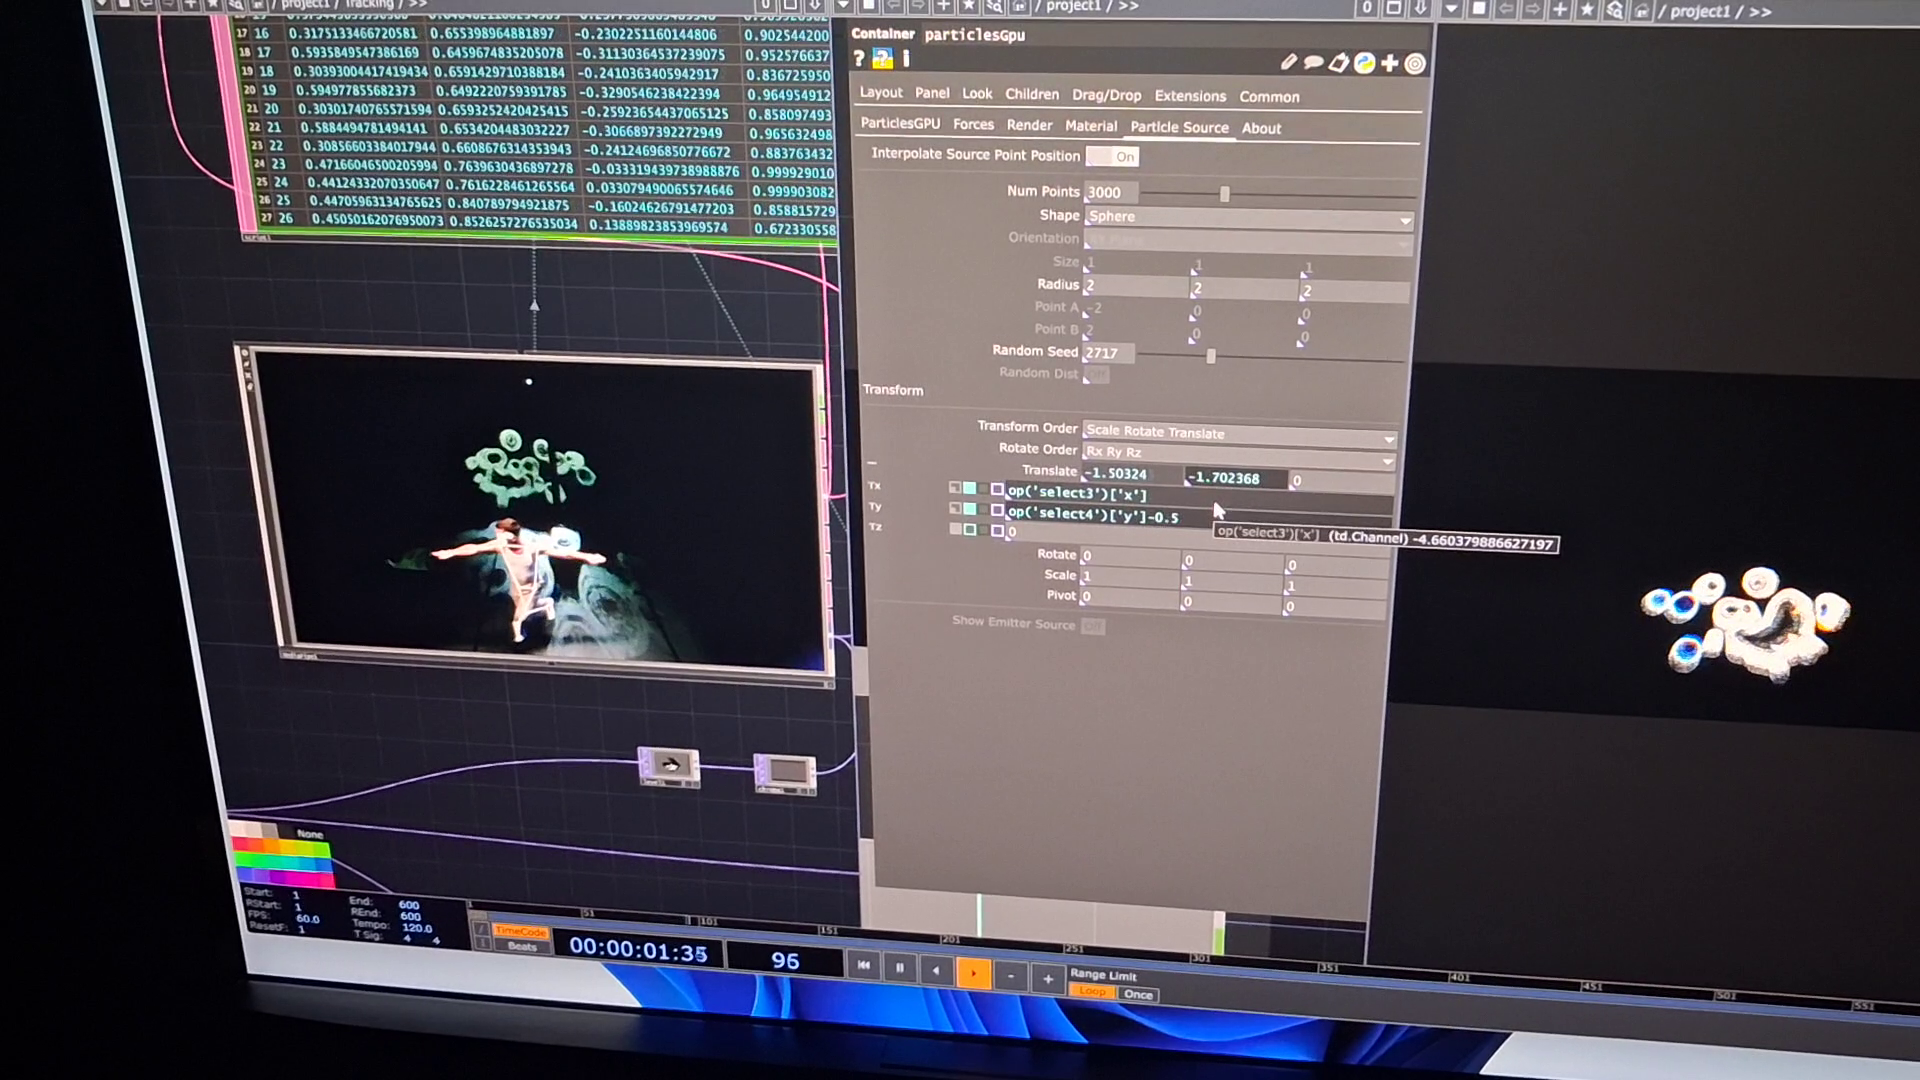
\includegraphics[width=0.6\textwidth,height=0.25\textheight,keepaspectratio]{images/HeadtrackingBubblesClearlyAtHeadLevelOnBackgroundBeamerMediaPipeSkeletonBeautifullyVisible.png}
   \caption{Endergebnis: Trotz Herausforderungen ein gutes Resultat}
   \label{fig:head_result}
\end{figure}

\begin{figure}[!htbp]
   \centering
   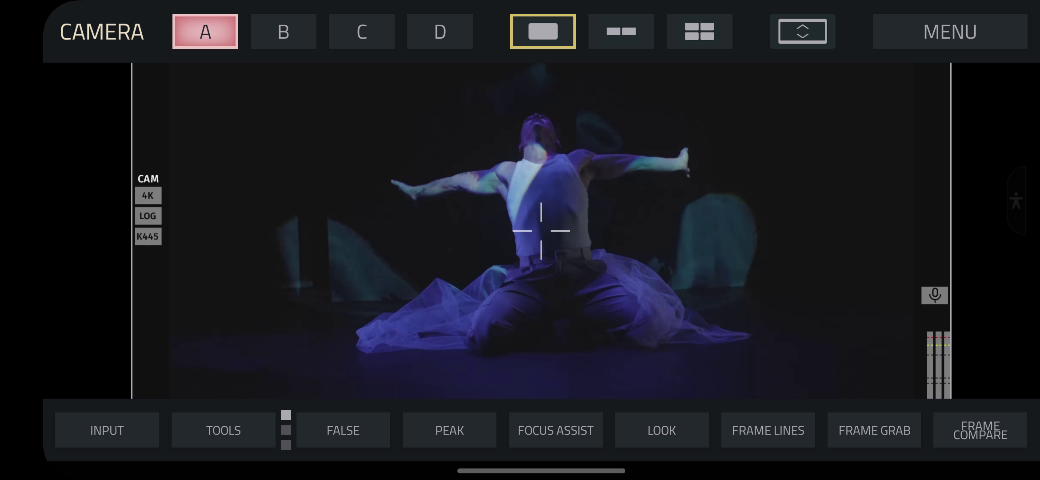
\includegraphics[width=0.6\textwidth,height=0.25\textheight,keepaspectratio]{images/HQCinemaCameraPerspectiveOfHandFireToTheSidesOfTheHands.png}
   \caption{Hand-Feuer Setup: Modulare Architektur bew�hrt sich}
   \label{fig:hand_fire_setup}
\end{figure}

\begin{figure}[!htbp]
   \centering
   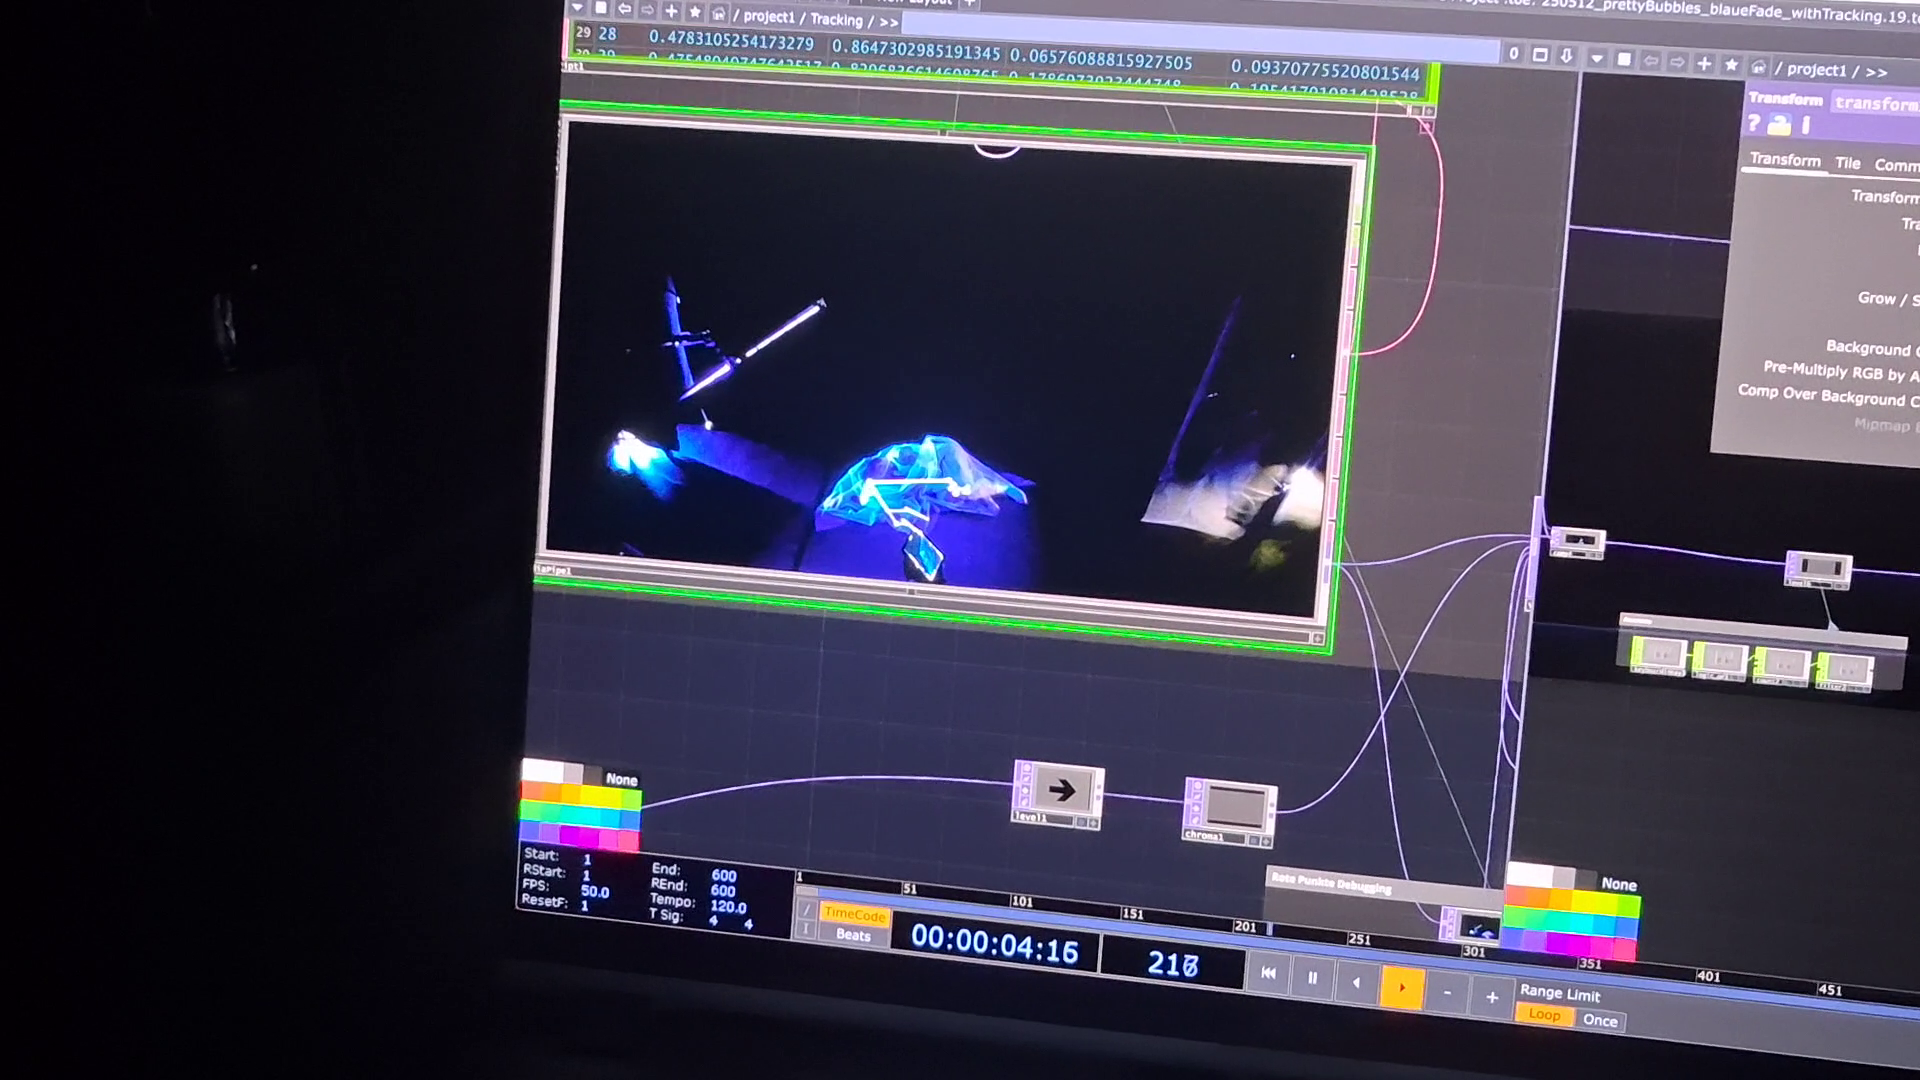
\includegraphics[width=0.6\textwidth,height=0.25\textheight,keepaspectratio]{images/DancerNotMediaPipeFoundCorrectlyWhenInClothOnFloor.png}
   \caption{Tracking-Problem: MediaPipe verliert Skelett-Erkennung bei Stoffverschleierung}
   \label{fig:cloth_tracking_issue}
\end{figure}

\begin{figure}[!htbp]
   \centering
   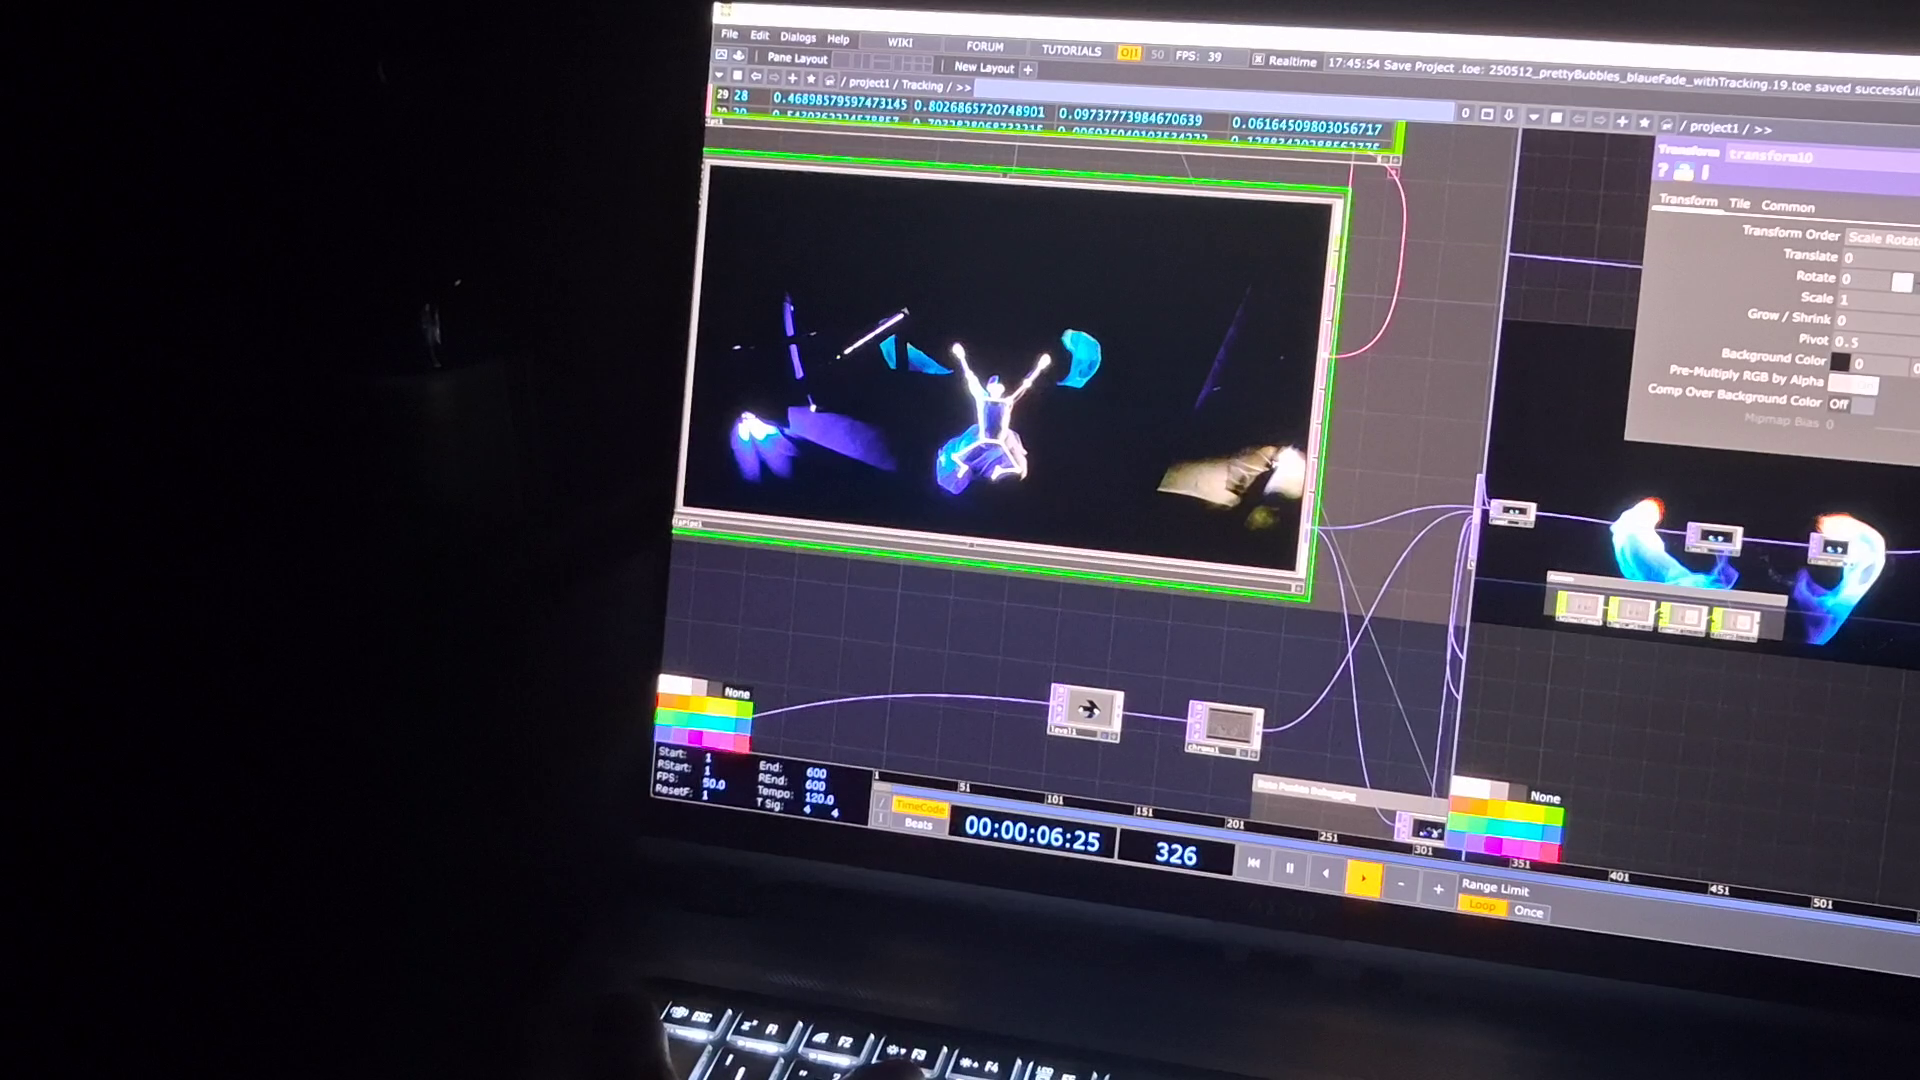
\includegraphics[width=0.6\textwidth,height=0.25\textheight,keepaspectratio]{images/dancerWithHandFireViewFromKinect.png}
   \caption{Hand-Feuer in Aktion: Blaue Partikel folgen den H�nden}
   \label{fig:hand_fire_action}
\end{figure}

\begin{figure}[!htbp]
   \centering
   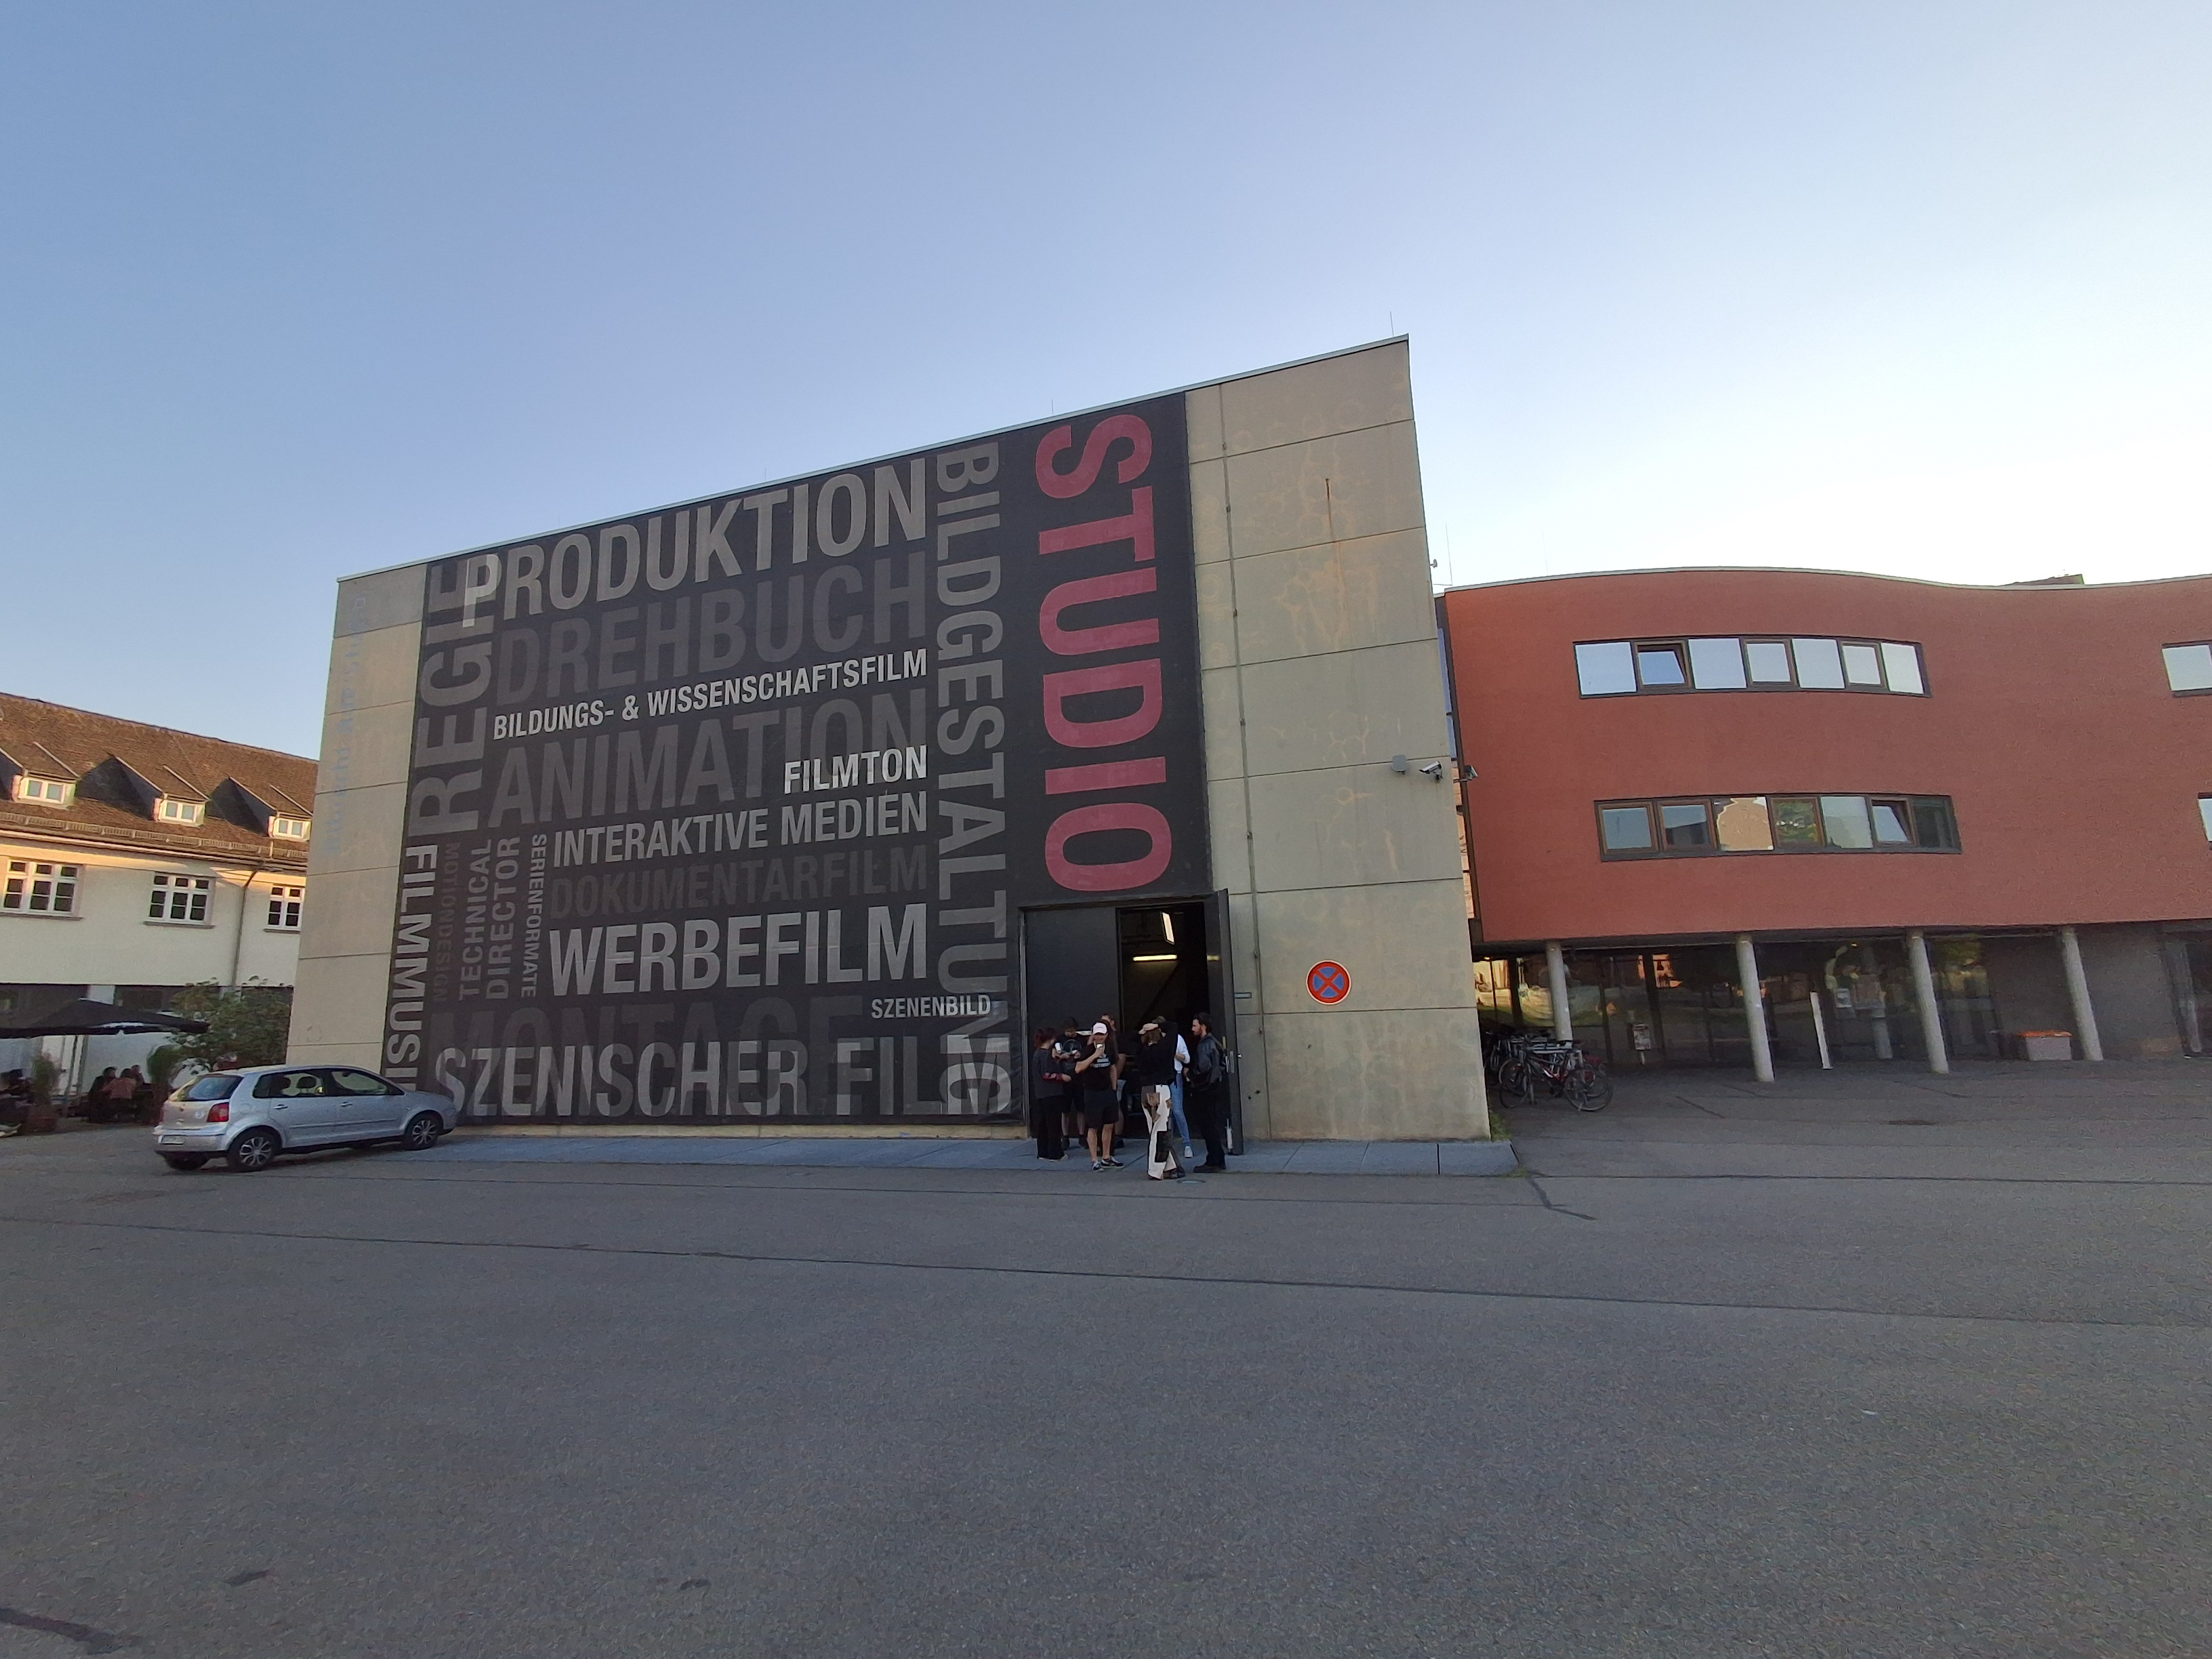
\includegraphics[width=0.6\textwidth,height=0.25\textheight,keepaspectratio]{images/onSetImages/WideShotOfOutsideOfStudioAfter2DayShoot.jpg}
   \caption{Produktionsabschluss: Au�enansicht des Albrecht-Ade-Studios nach zweit�giger Drehzeit}
   \label{fig:studio_exterior}
\end{figure}

\begin{figure}[!htbp]
   \centering
   \includegraphics[width=0.6\textwidth,height=0.25\textheight,keepaspectratio]{images/onSetImages/wideStudioShotPreparingTopDownSpikeShot.jpg}
   \caption{Teamarbeit: Professionelle Crew integriert M.A.S.K. in den Workflow}
   \label{fig:crew_setup}
\end{figure}

\begin{figure}[!htbp]
   \centering
   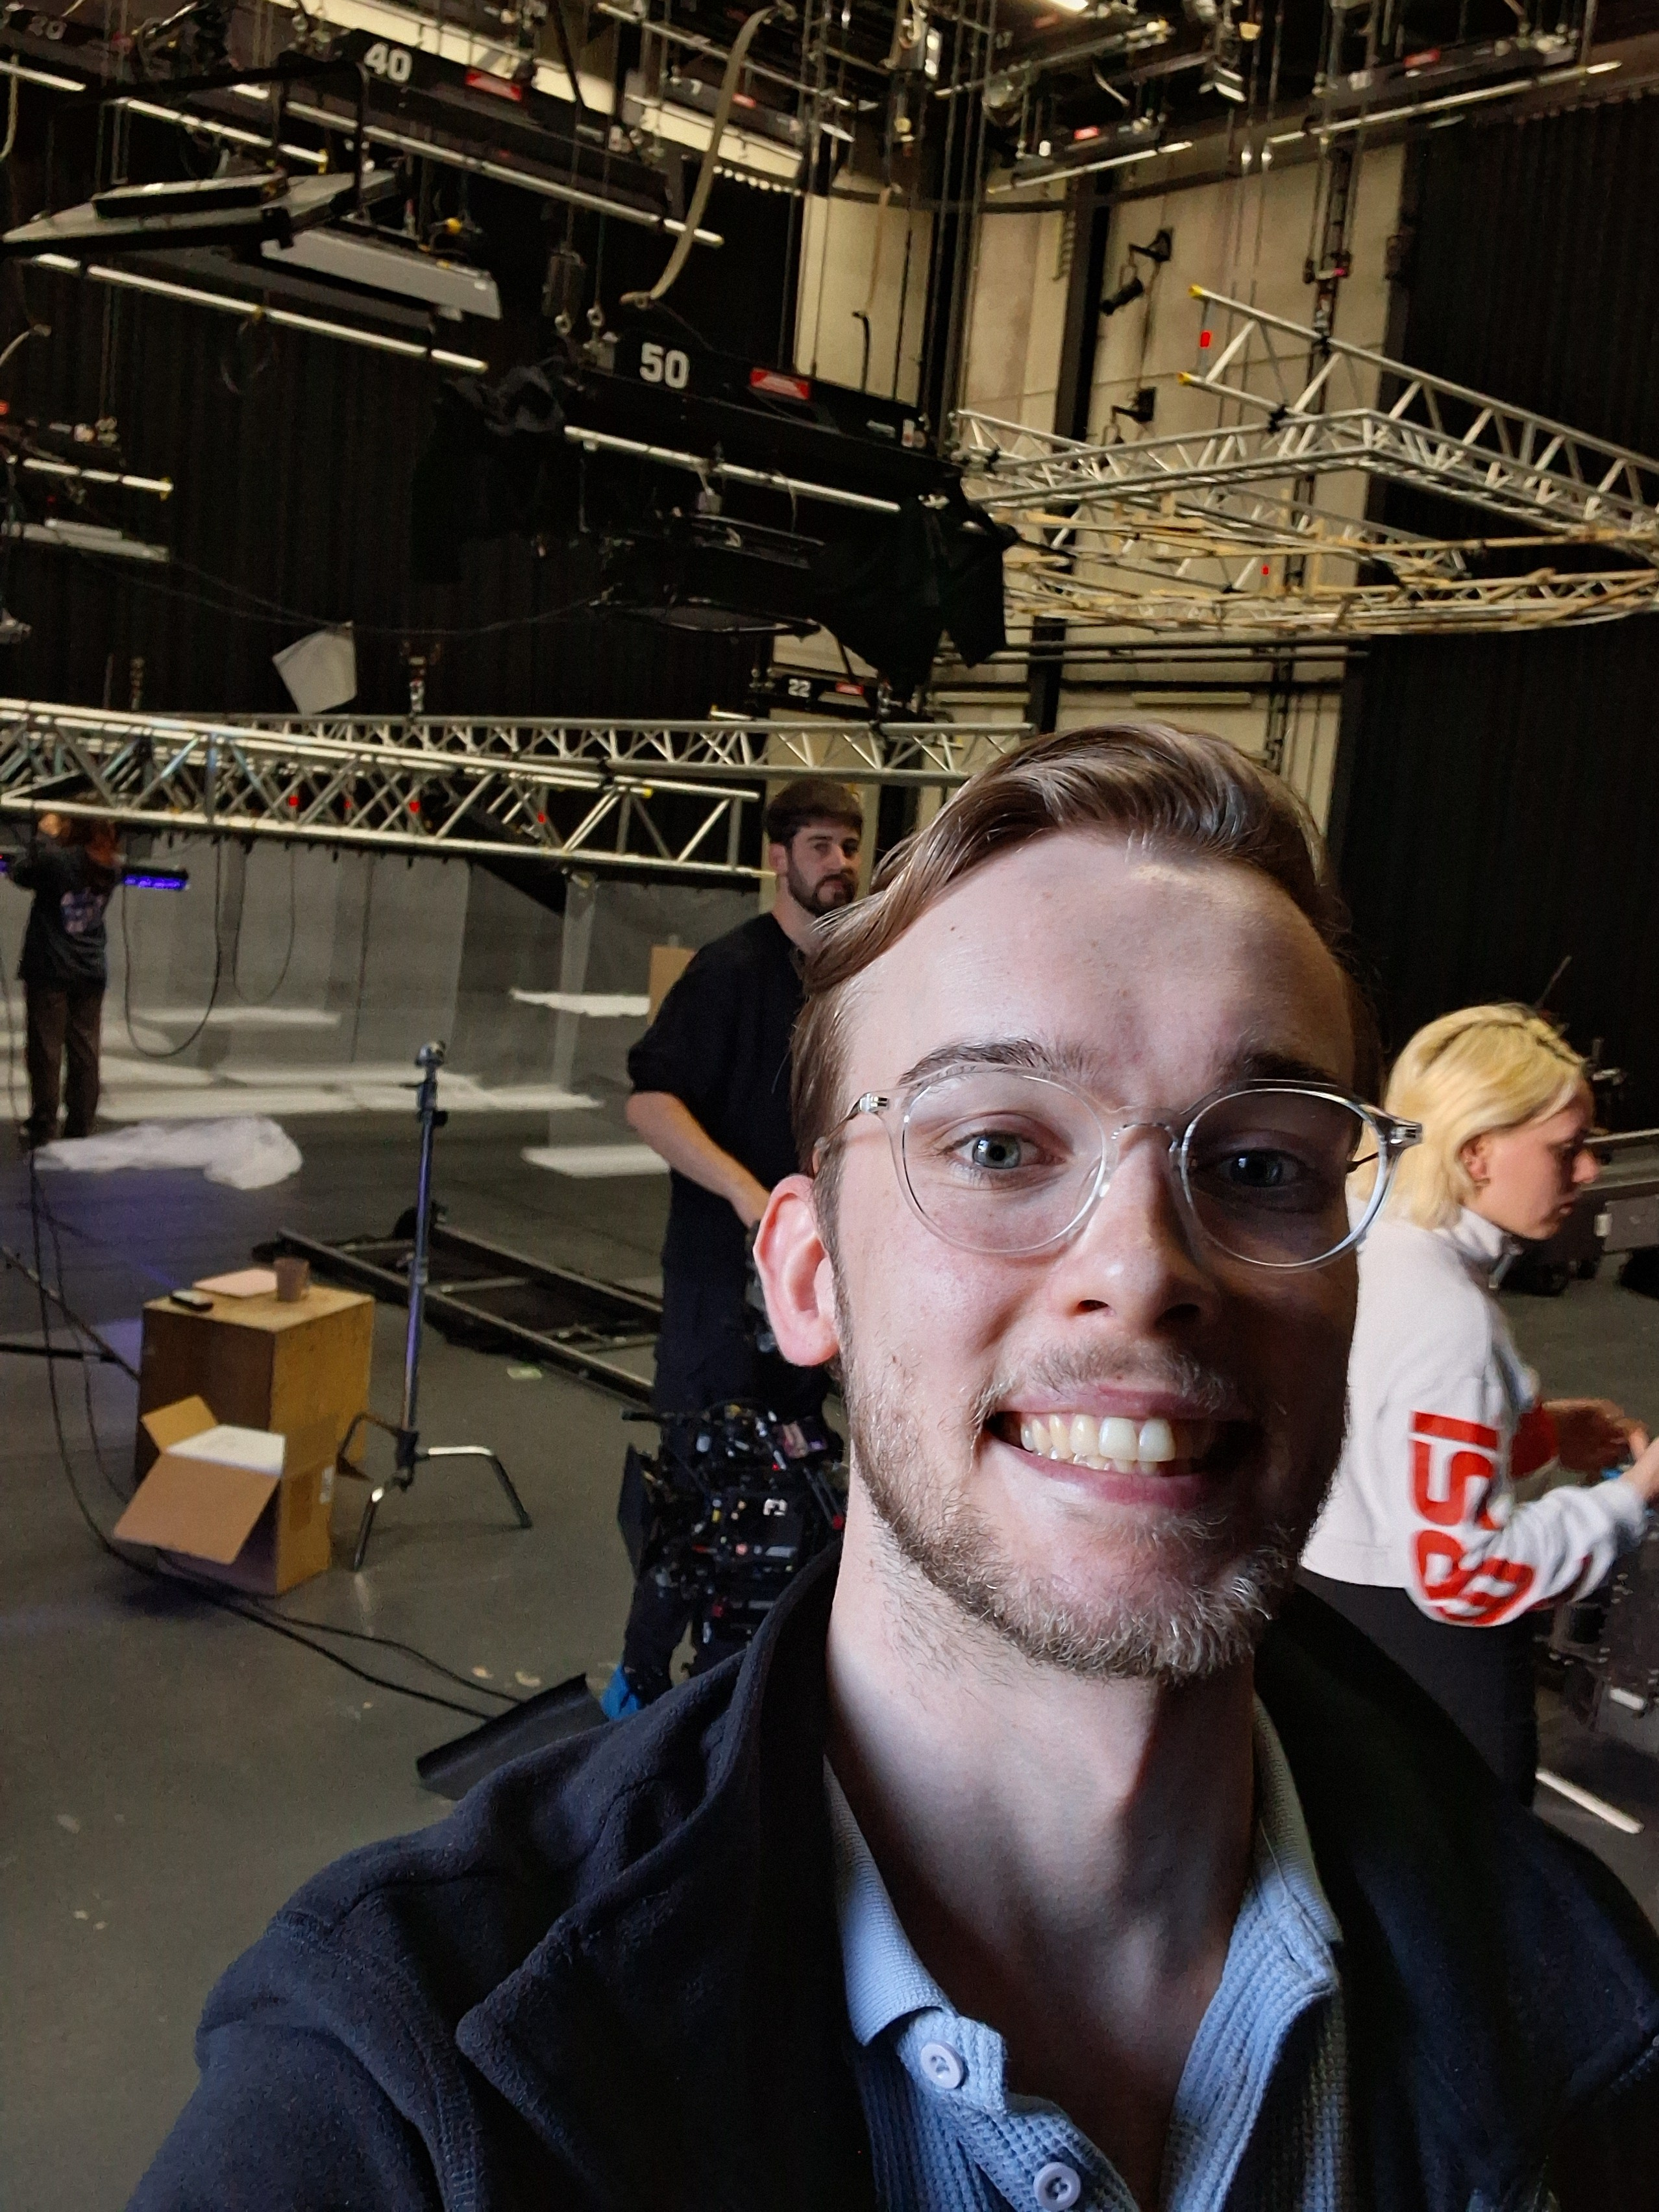
\includegraphics[width=0.6\textwidth,height=0.25\textheight,keepaspectratio]{images/onSetImages/MartySmileyIntoCameraOnSet.jpg}
   \caption{Teamdynamik: Entspannte Atmosph�re zwischen den Takes trotz technischer Herausforderungen}
   \label{fig:team_atmosphere}
\end{figure}

\begin{figure}[!htbp]
   \centering
   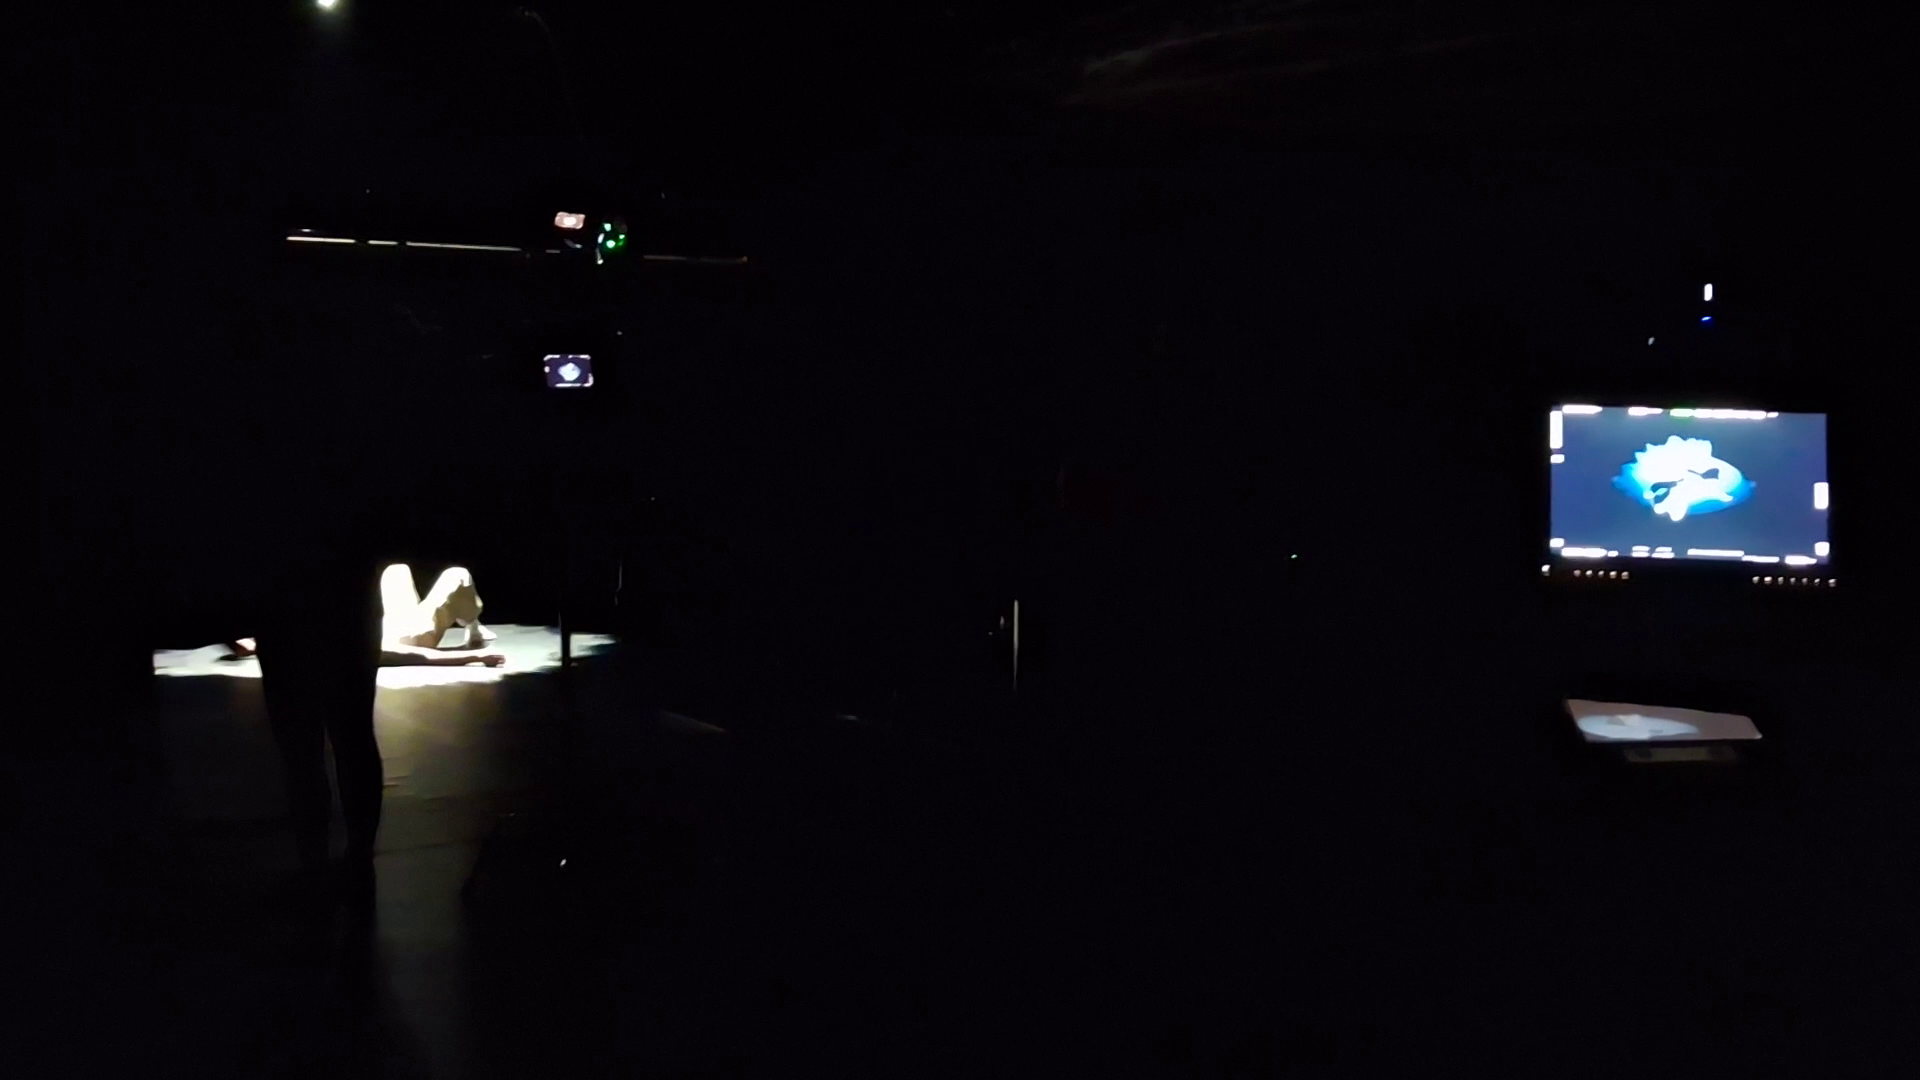
\includegraphics[width=0.6\textwidth,height=0.25\textheight,keepaspectratio]{images/BTS_TopDown_DancerAndProducer.png}
   \caption{Behind the Scenes: T�nzer mit professioneller Lichttechnik und Producer-Ansicht}
   \label{fig:studio_wide}
\end{figure}